\documentclass[../Main.tex]{subfiles}

\begin{document}
    \subsection{General Testing}
        These tests were conducted during the programming of the solution.
        \subsubsection{Generating rooms from images}
            \begin{figure}[hbt!]
                \centerline{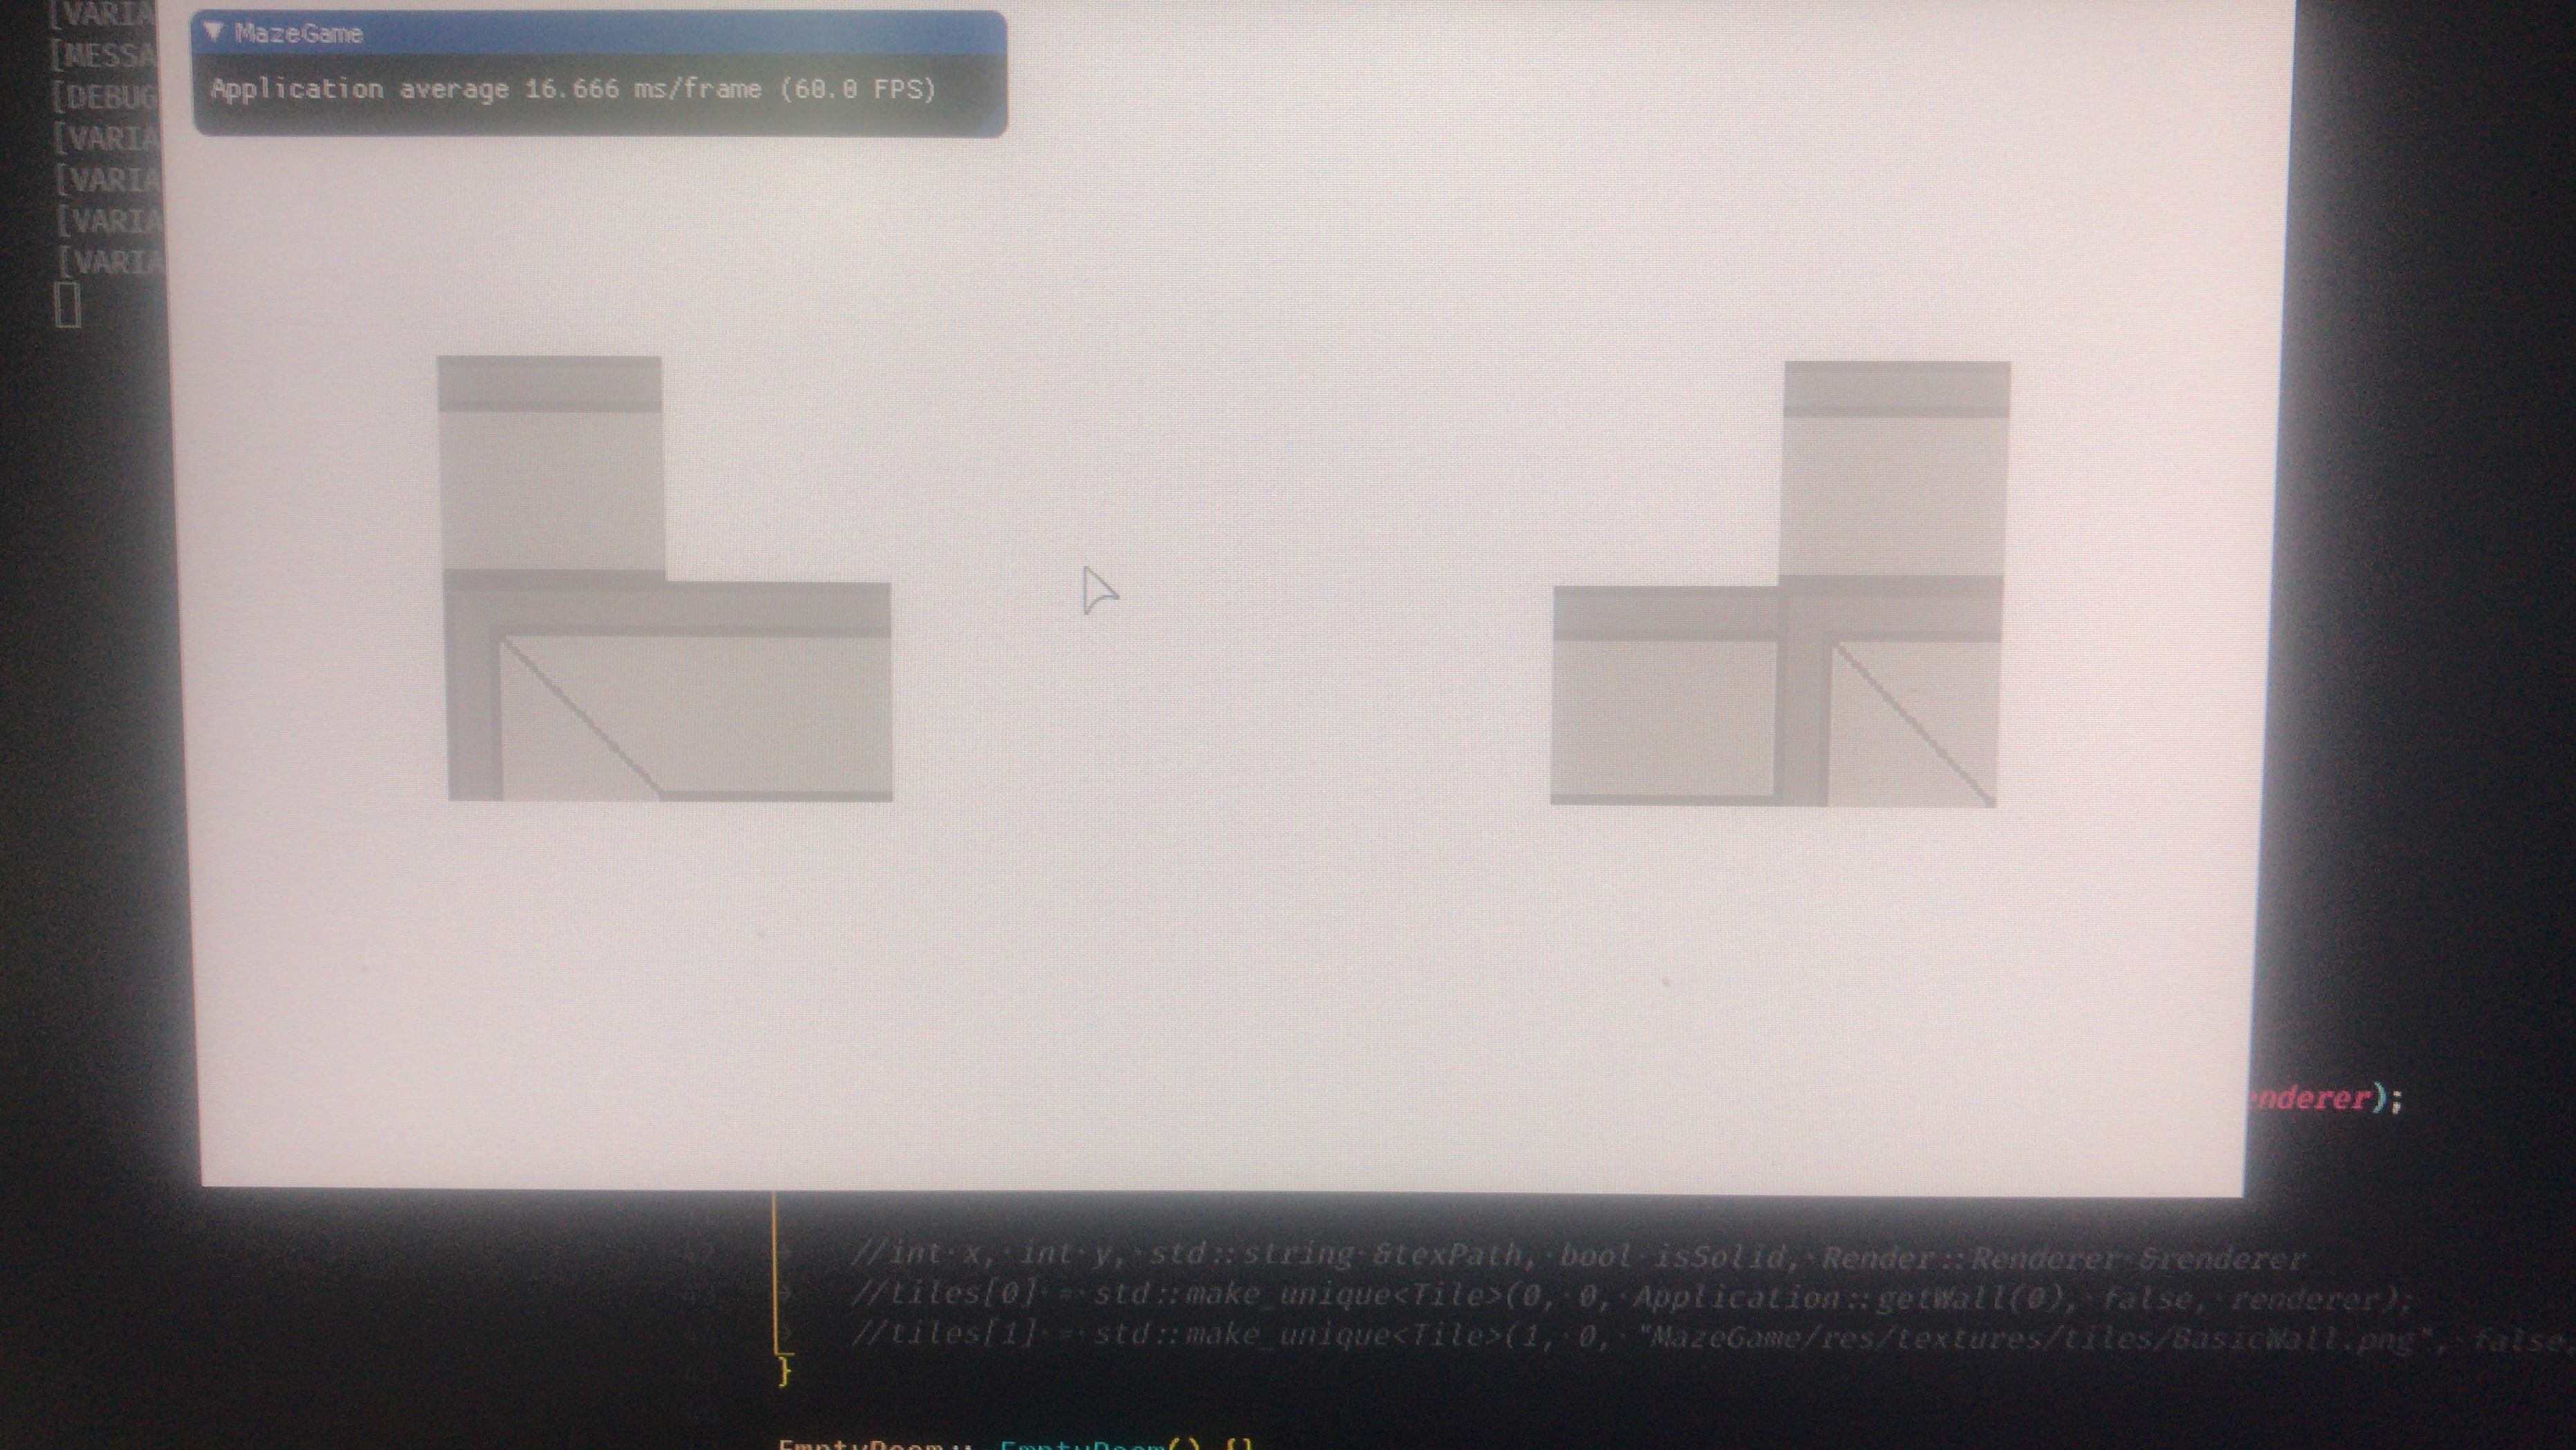
\includegraphics[scale=0.1]{img/Testing/General/Room Not rendering.jpg}}
                \caption{Room incorrectly rendering}
                \label{fig:roomNotRendering1}
            \end{figure}
            \begin{figure}[hbt!]
                \centerline{\includegraphics[scale=0.1]{img/Testing/General/Room Not rendering2.jpg}}
                \caption{Room incorrectly rendering}
                \label{fig:roomNotRendering2}
            \end{figure}
            As shown in Figure \ref{fig:roomNotRendering1} and Figure \ref{fig:roomNotRendering2}, when setting up the room generation from a bitmap file, they were either not rendering all the tiles or not generating the tiles correctly. After a bit of digging, I noticed that only the walls and corners were being rendered, which could suggest that the textures were not being loading correctly. I then noticed that the filename was labelled incorrectly for both the corner and the floor tiles, which I then promptly fixed which resulted in all the tiles being rendered.
            \clearpage
            \begin{figure}[hbt!]
                \centerline{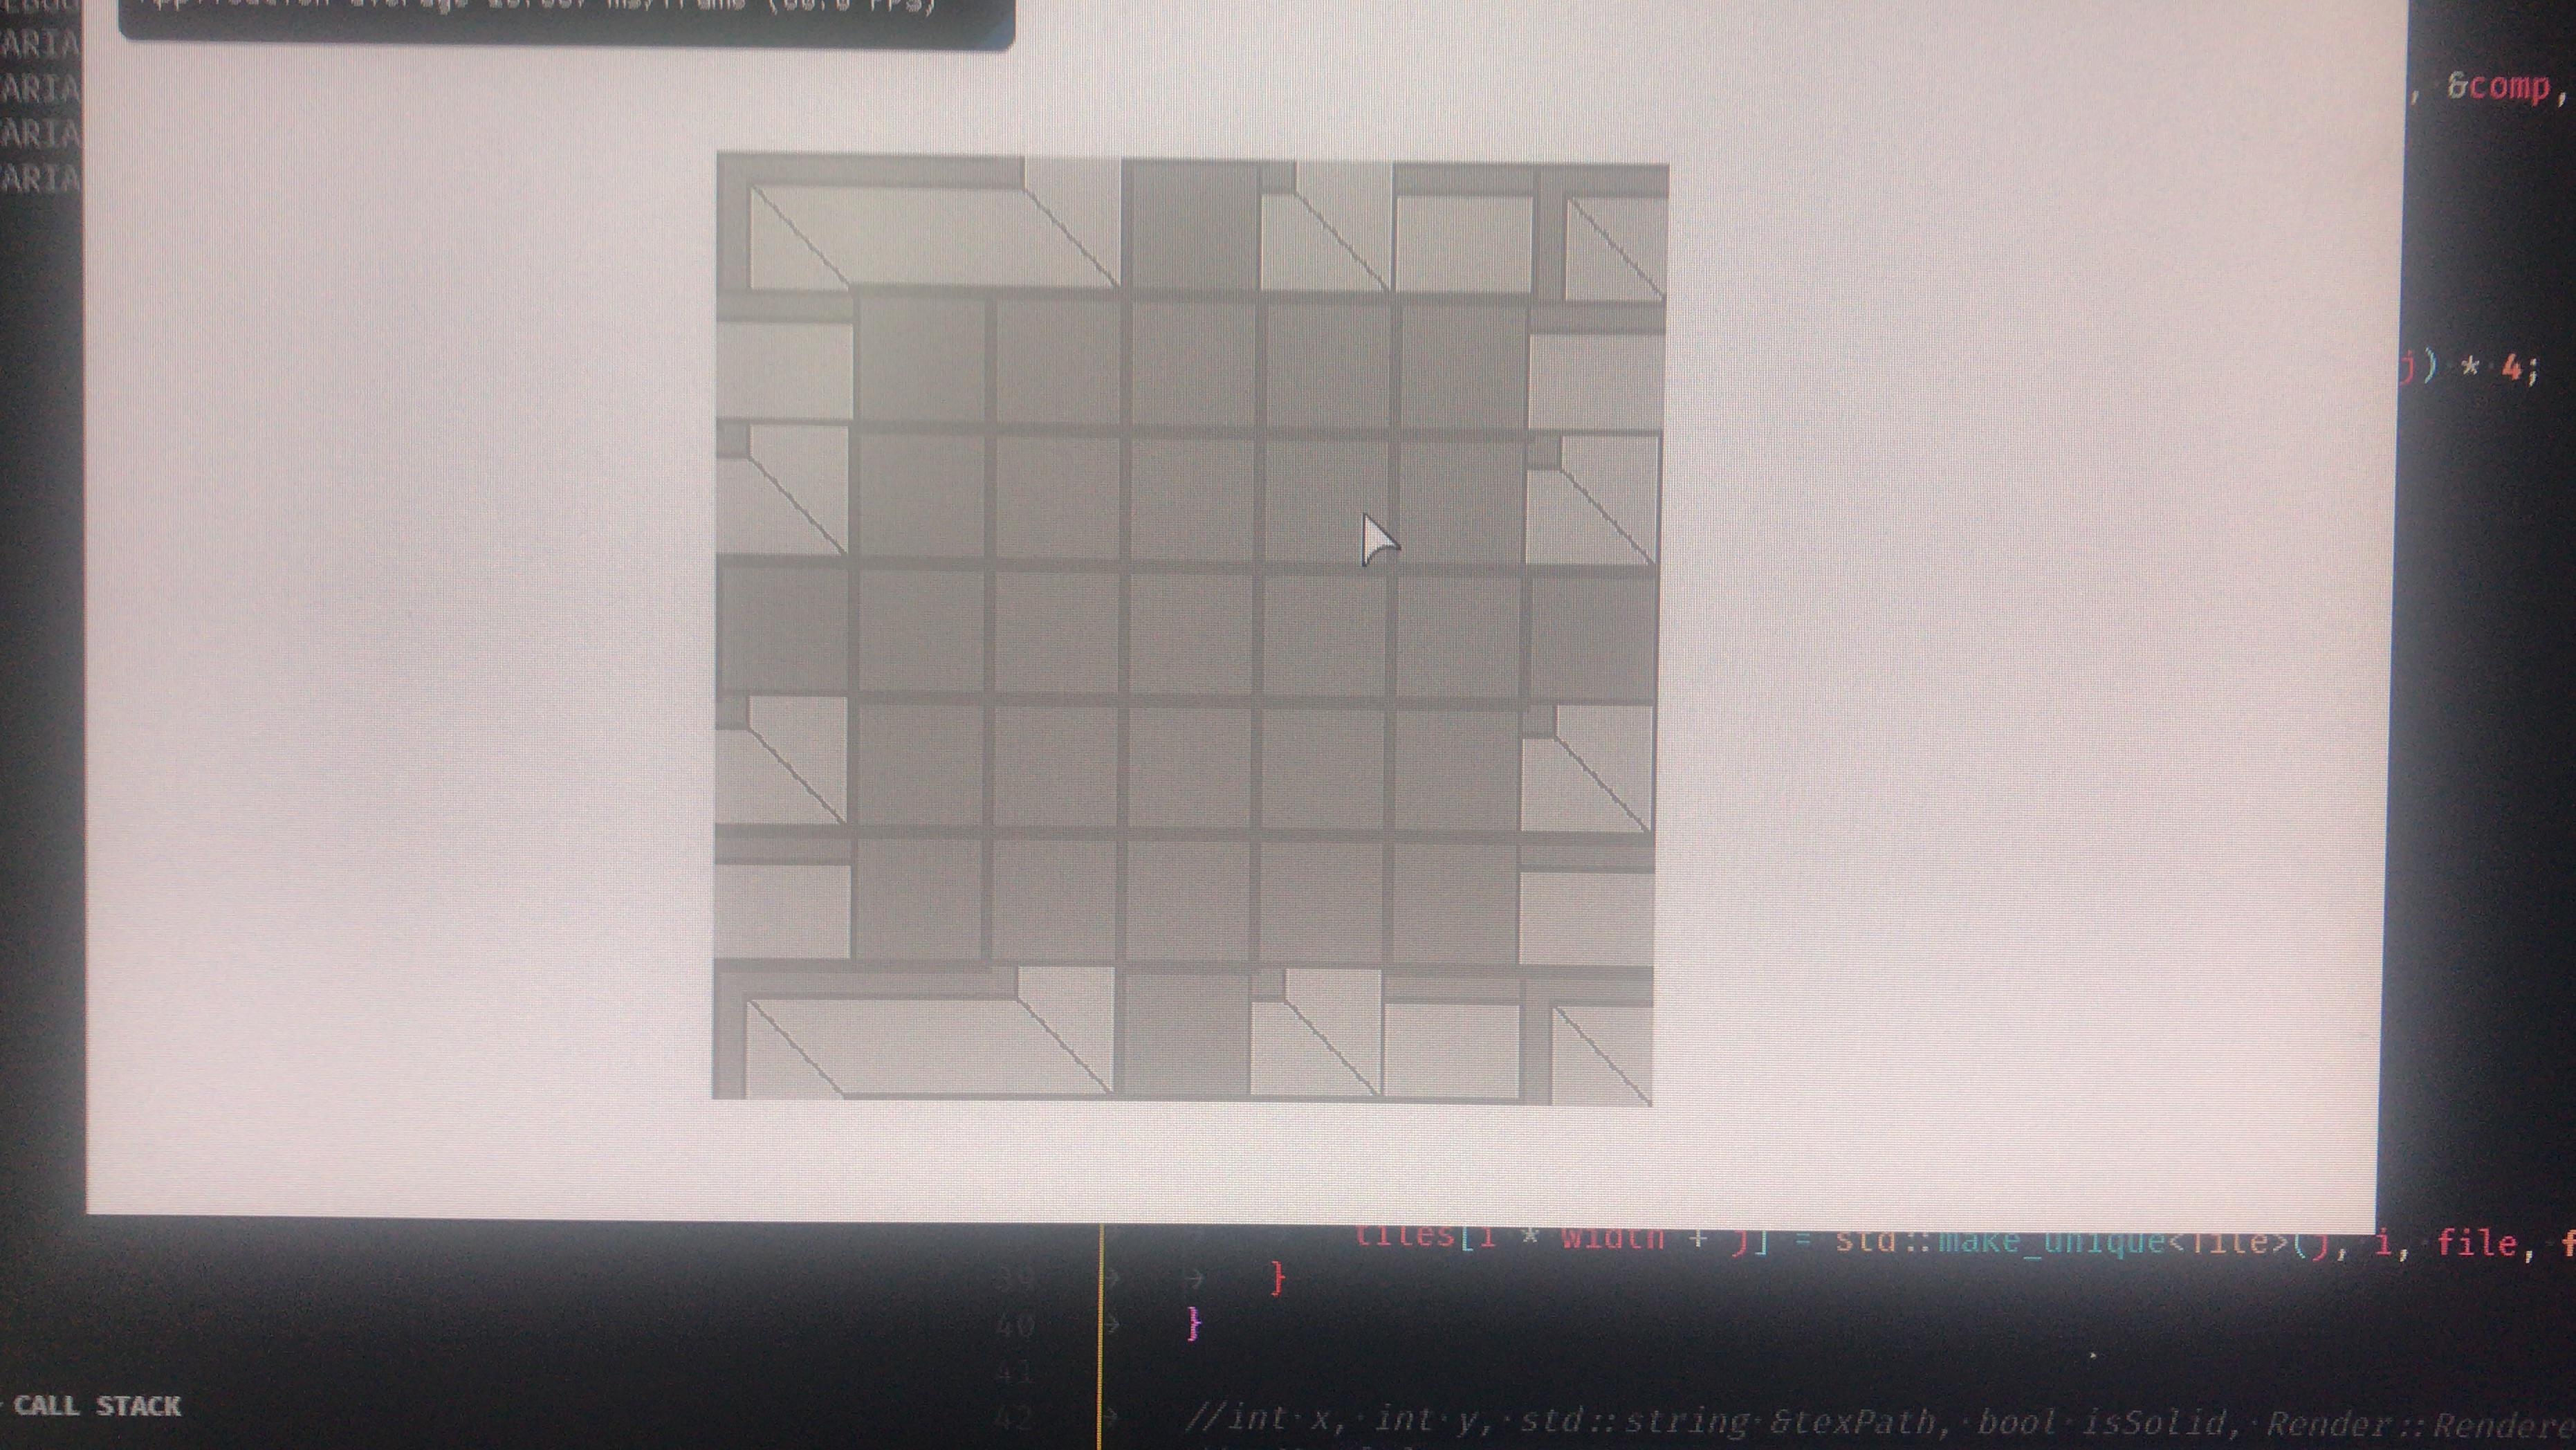
\includegraphics[scale=0.1]{img/Testing/General/Incorrect rotation.jpg}}
                \caption{Incorrect rotation of the tiles}
                \label{fig:IncorrectRotation}
            \end{figure}
            As shown in Figure \ref{fig:IncorrectRotation}, I had an issue that the tiles were not rotated correctly when rendering (They all had the same rotation). This was a very quick fix as I realised I had not created any code to calculate the rotation of the wall based off the position, which I then quickly added which resulted in the tiles being correctly rotated.

        \subsubsection{Maze generating incorrectly}
            \begin{figure}[hbt!]
                \centerline{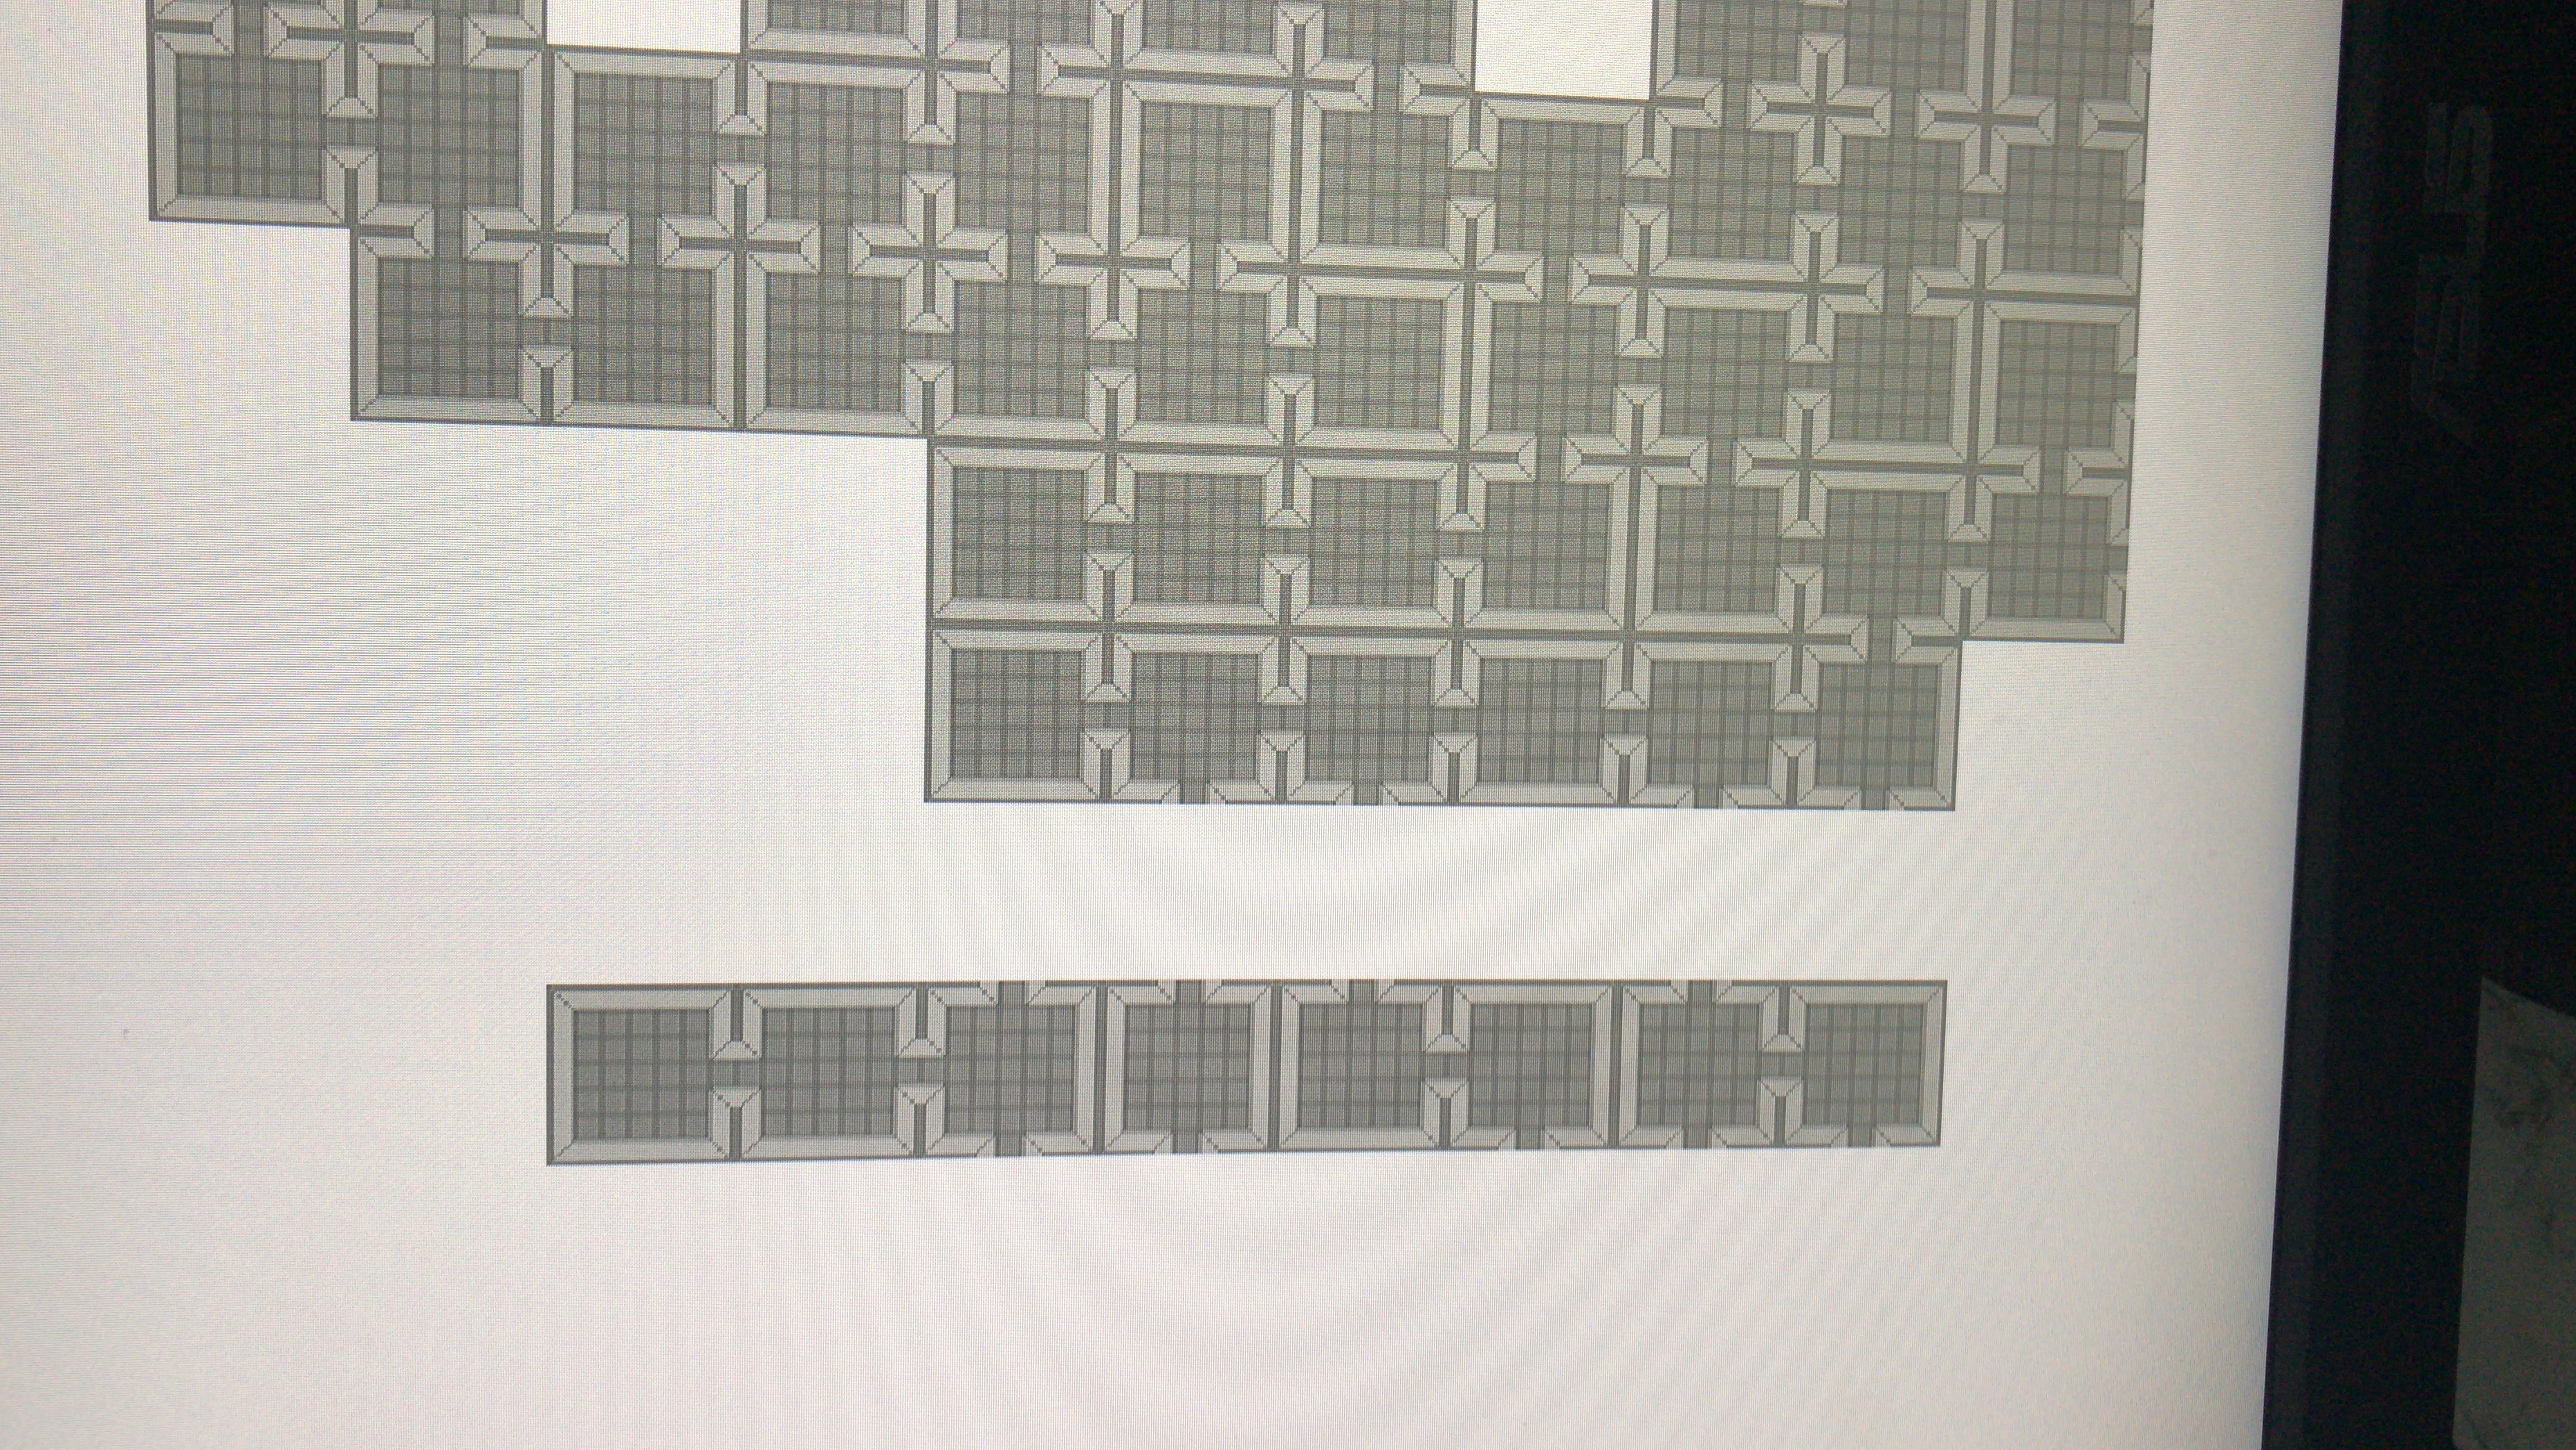
\includegraphics[scale=0.1]{img/Testing/General/Maze Gen Issue.jpg}}
                \caption{Maze generation leaving gaps}
                \label{fig:MazeGenIssue}
            \end{figure}
            As shown in Figure \ref{fig:MazeGenIssue}, after moving south or west, the maze would sometimes skip a row, leaving a blank row. To solve this, I went through the code for setting up the south, and west movement and generation, which I then noticed that when looping the offset back from 0 to the top. Instead of checking if the offset had been on 0, it was checking if the offset had been on 1, which meant that it was completely skipping a row when generating. So once that was fixed it was generating perfectly fine.

        \clearpage
        \subsubsection{Upgrading the rendering}
            \begin{figure}[hbt!]
                \centerline{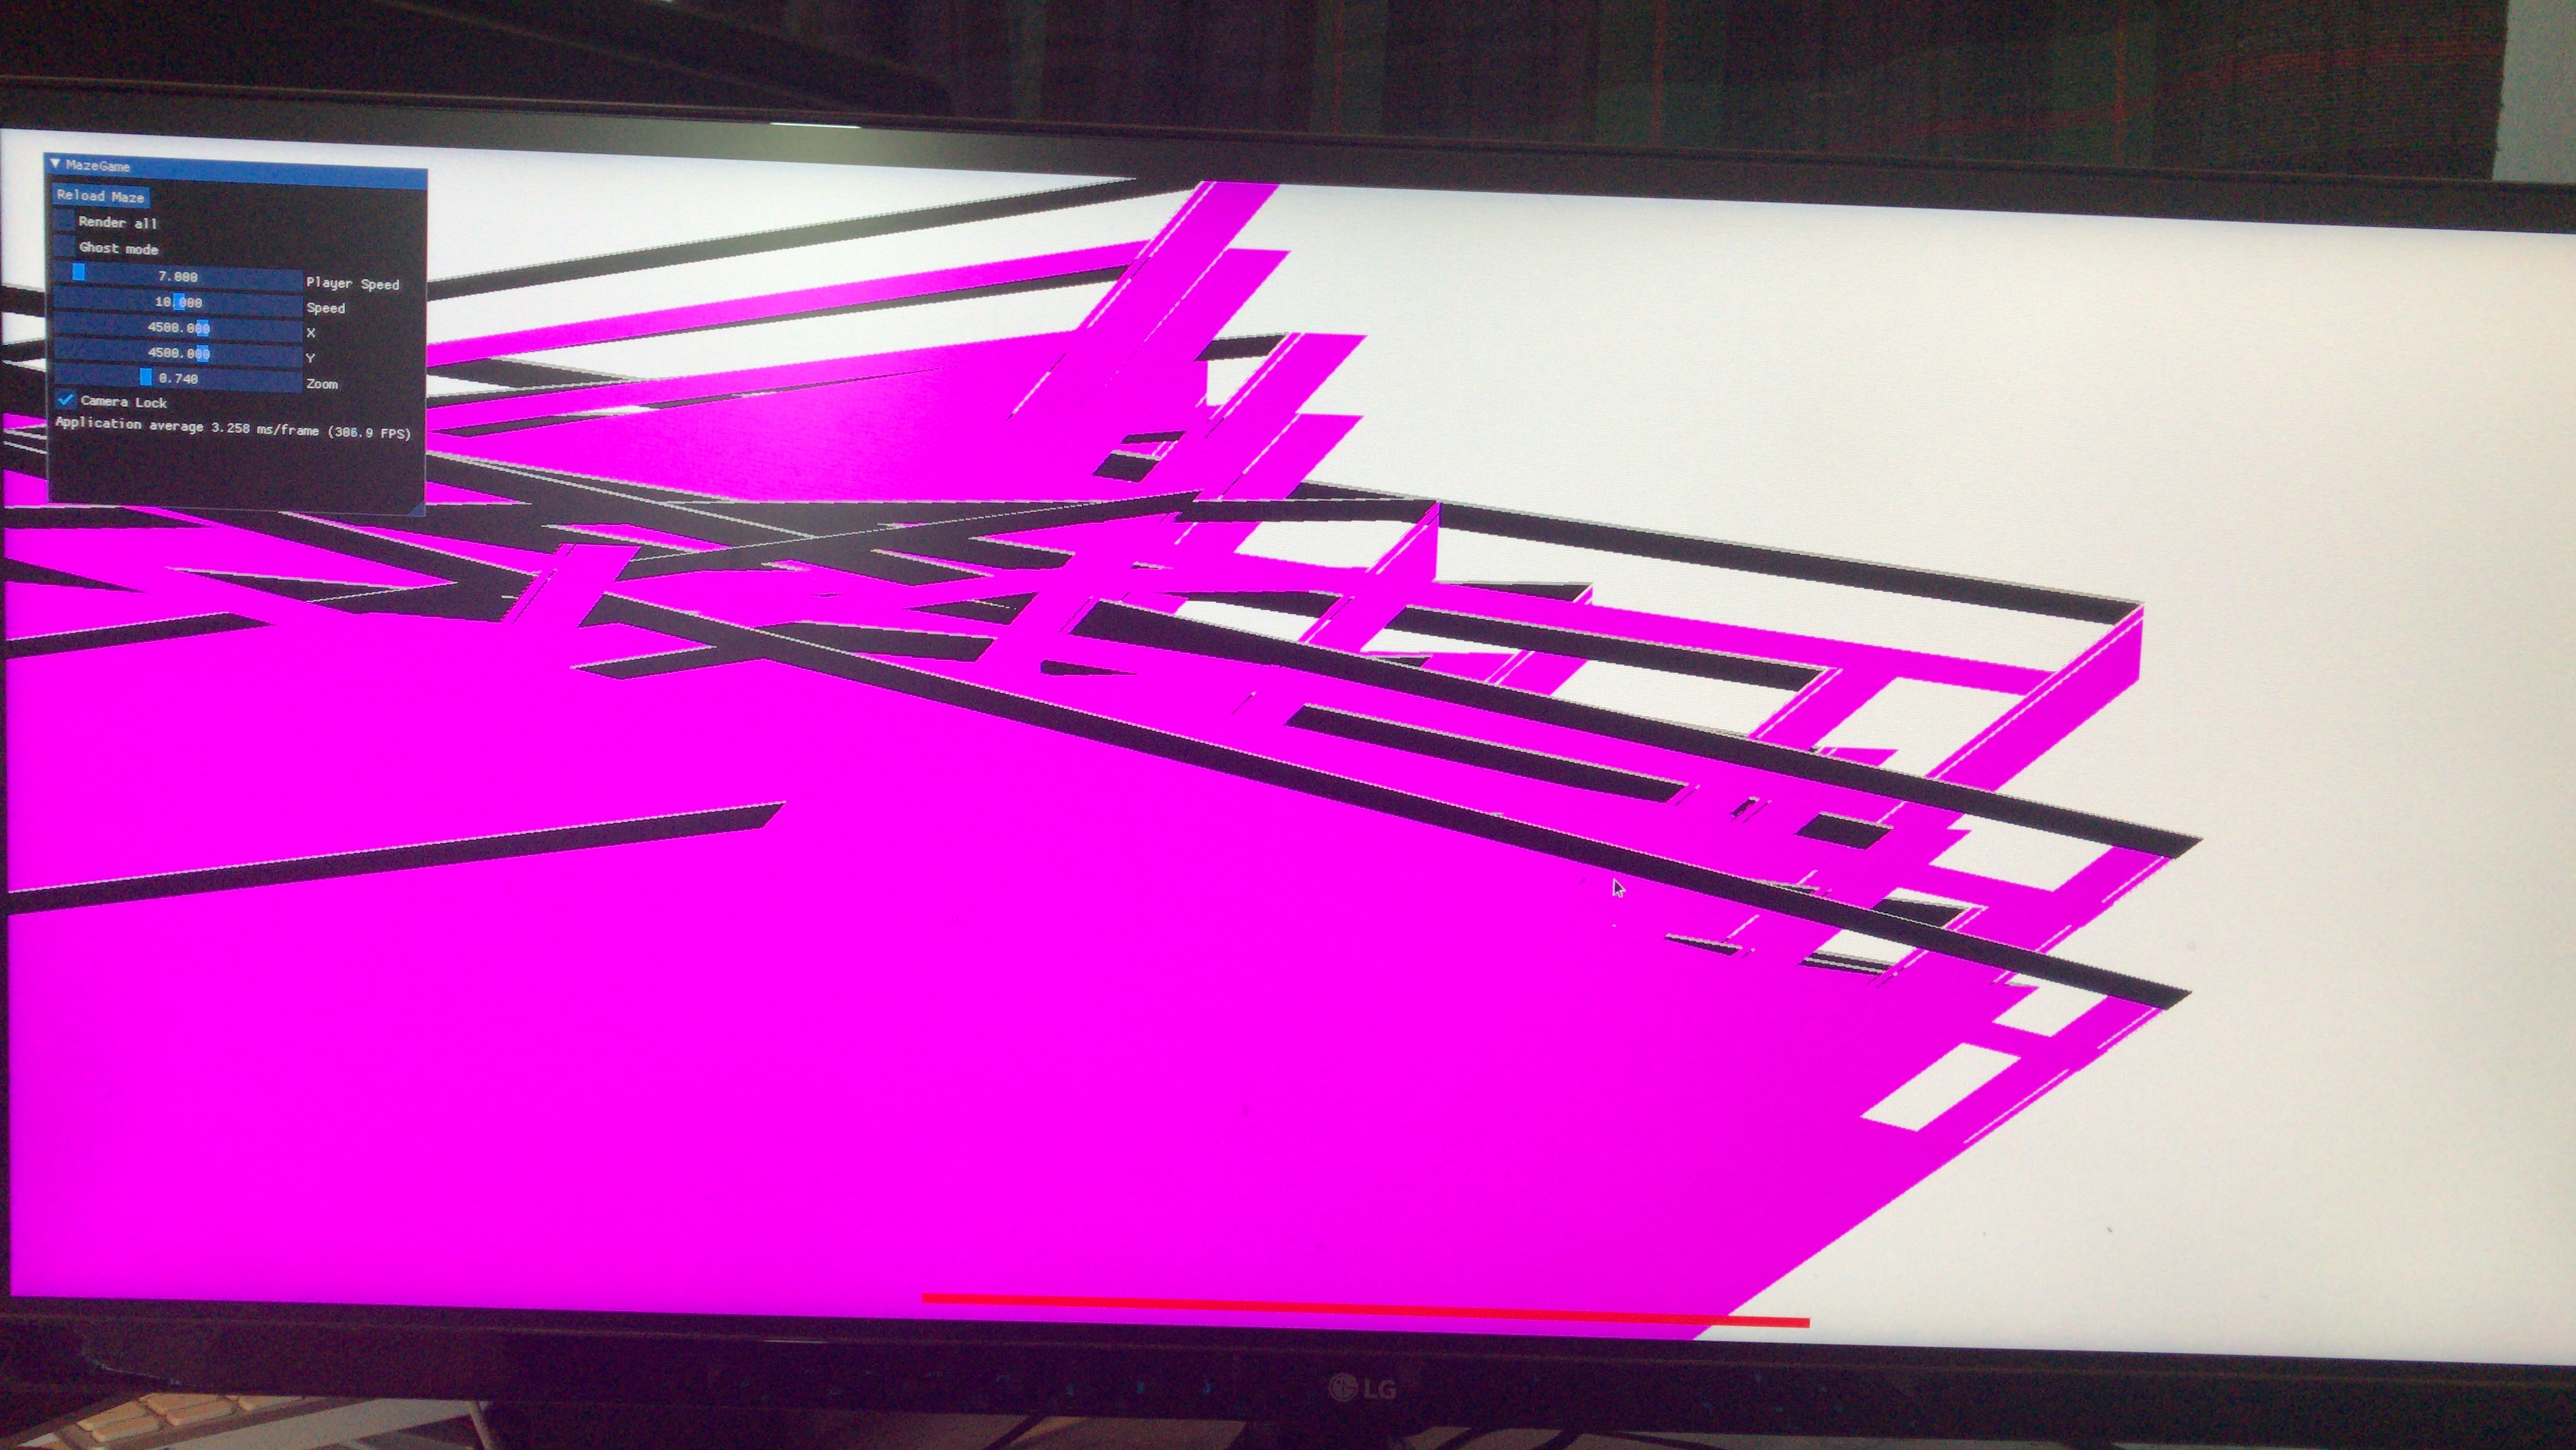
\includegraphics[scale=0.09]{img/Testing/General/ShaderIssue.jpg}}
                \caption{Incorrect shader positions}
                \label{fig:IncorrectShaderPos}
            \end{figure}
            \begin{figure}[hbt!]
                \centerline{\includegraphics[scale=0.085]{img/Testing/General/SimpleMaze.png}}
                \caption{Incorrect shader parameters}
                \label{fig:IncorrectShader}
            \end{figure}
            \begin{figure}[hbt!]
                \centerline{\includegraphics[scale=0.09]{img/Testing/General/Not refreshing buffer2.jpg}}
                \caption{Incorrect sprites rendered}
                \label{fig:IncorrectSprite1}
            \end{figure}
            \clearpage
            \begin{figure}[hbt!]
                \centerline{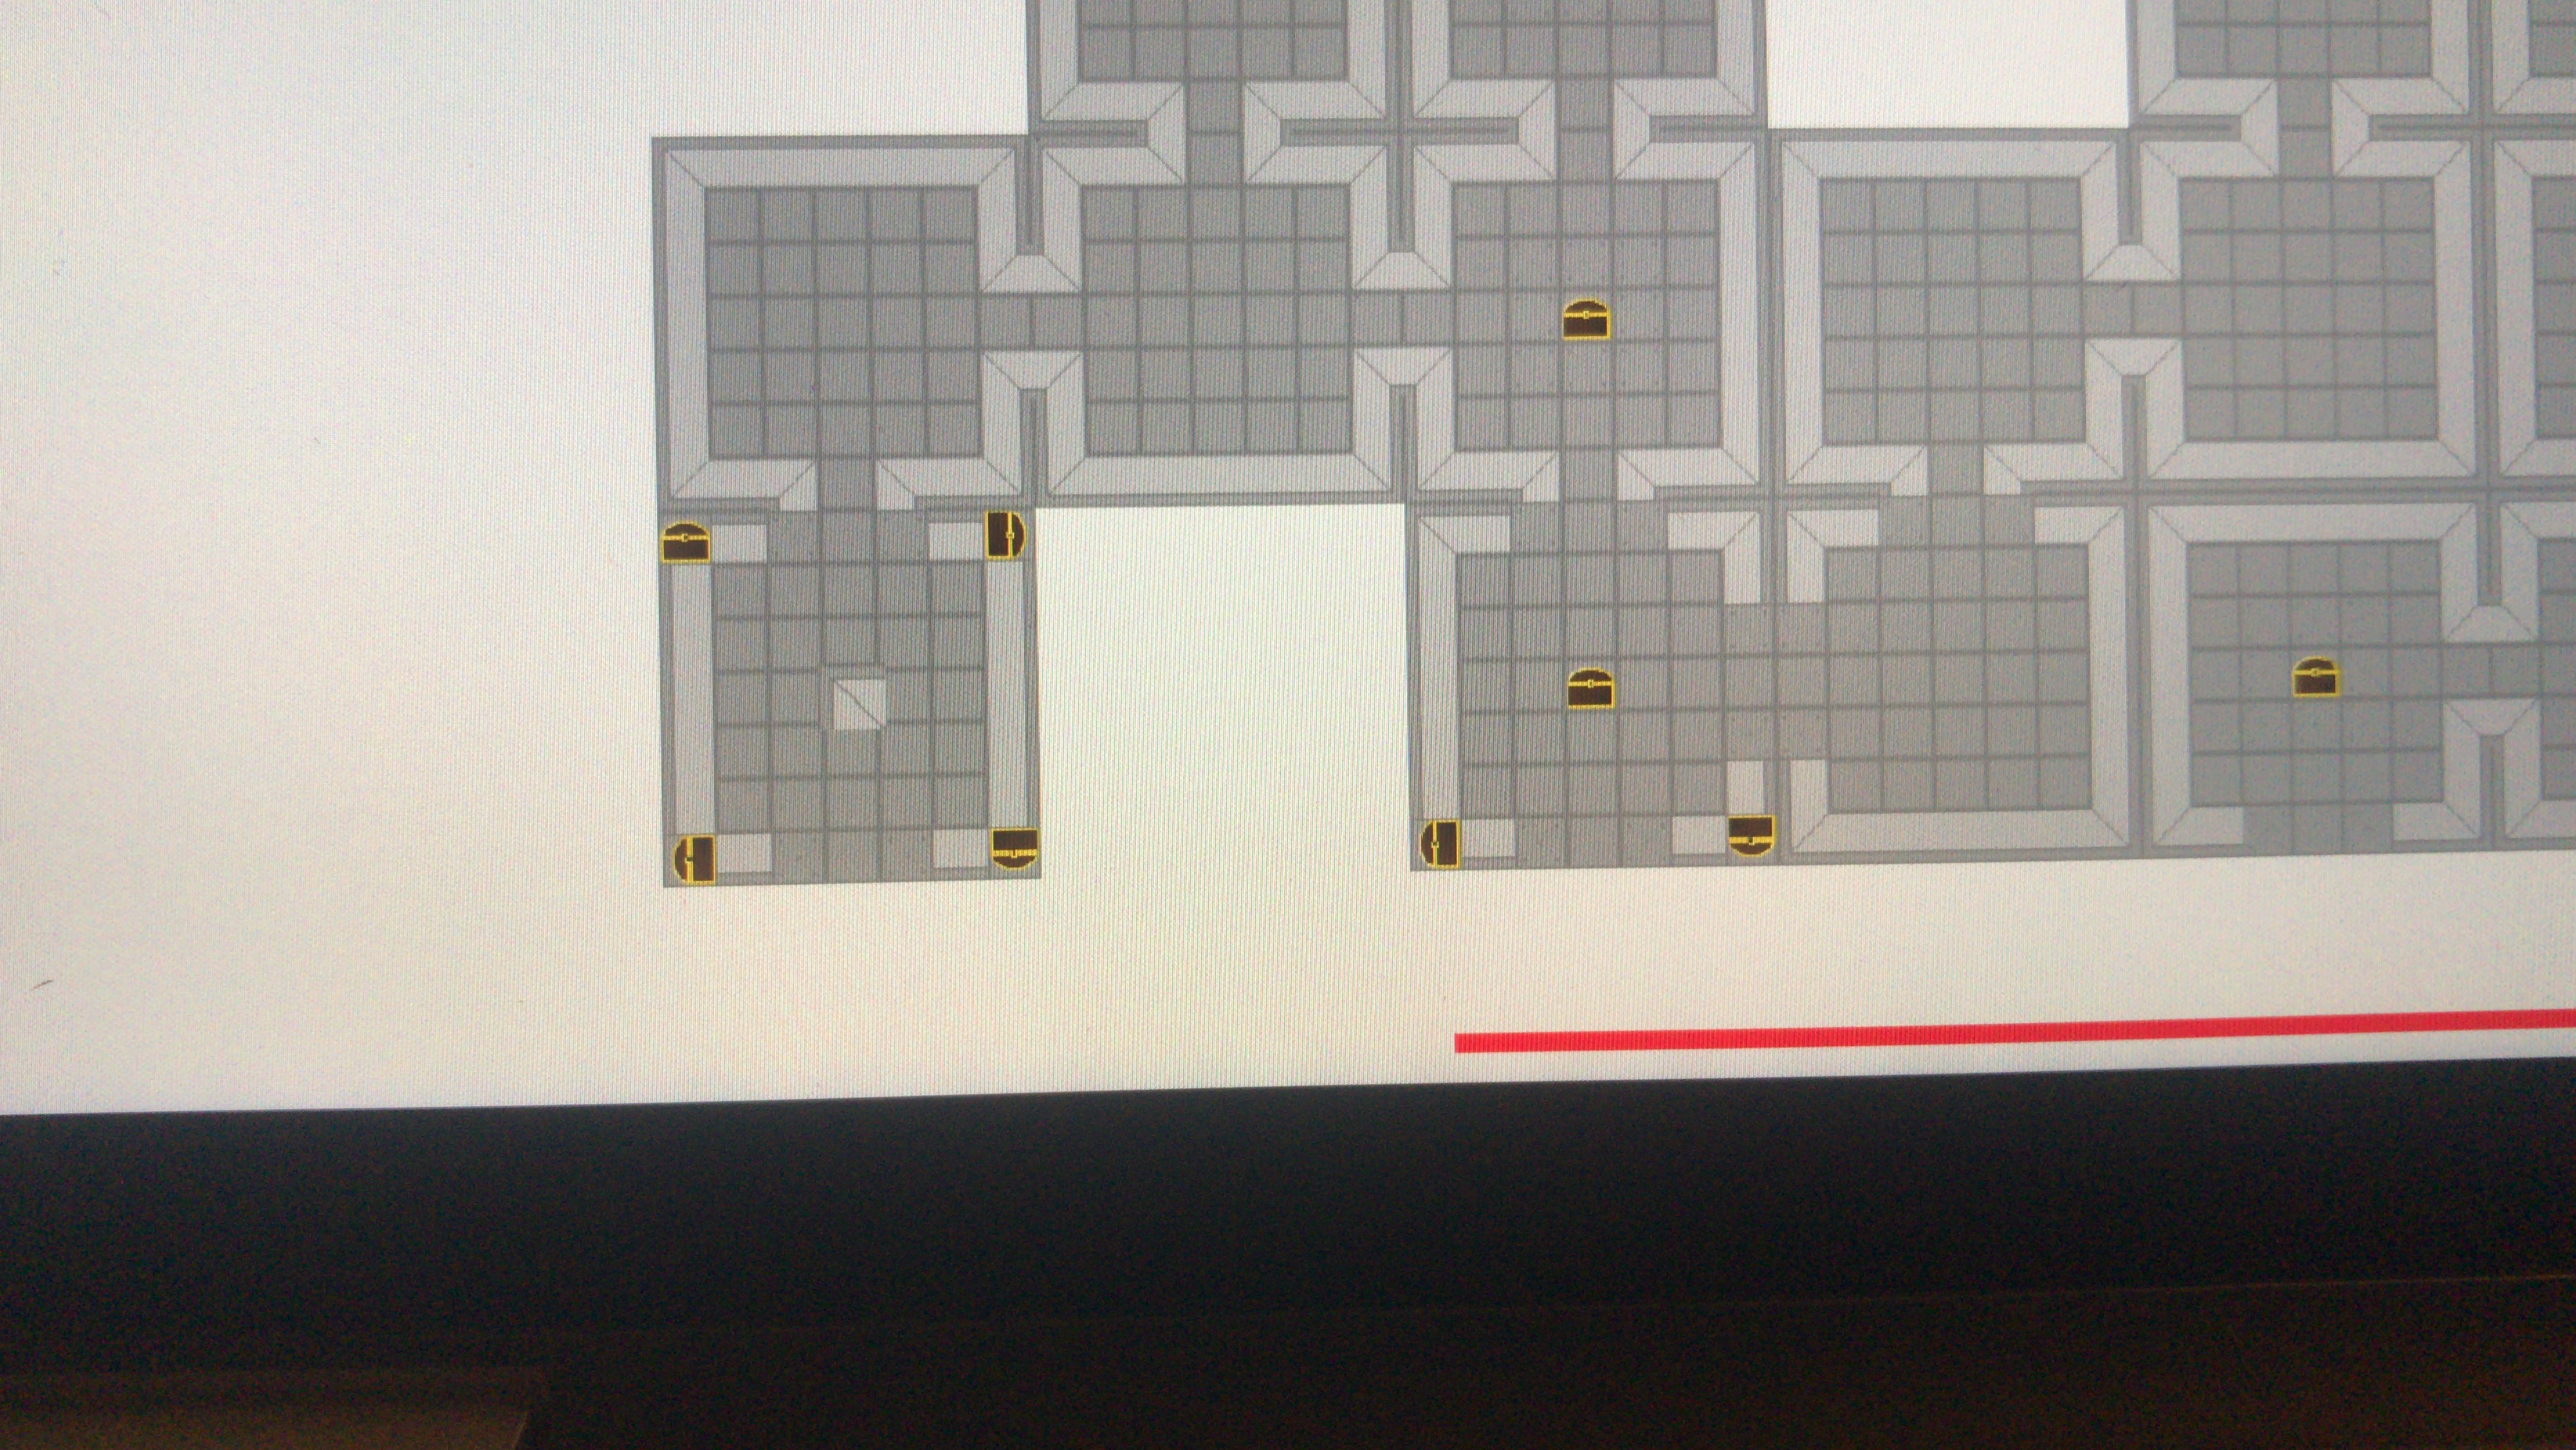
\includegraphics[scale=0.09]{img/Testing/General/Not refreshing buffer.jpg}}
                \caption{Incorrect sprites rendered}
                \label{fig:IncorrectSprite2}
            \end{figure}
            As shown in the figures above, I ran into many issues when rendering.

            In Figure \ref{fig:IncorrectShaderPos}, you can see just a mass of random pink lines. These lines would shift and change randomly as you moved the camera to around. After a lot of digging I noticed that, after moving the sprite rendering function as well as changing the structs that were used to store the buffer, I had used the incorrect size when adding to the buffer, which resulted in random shapes to be formed.

            In Figure \ref{fig:IncorrectShader}, you can see the sprites were rendered completely incorrectly, with when you zooming in and out, it resulting in them change slightly, from just solid blocks of one colour. I then noticed that, each sprite had a unique colour when rendering, which let me to find out that when storing the sprite in the struct, I had mixed up the order of the parameters for the shader, which resulted in the incorrect coordinates used for the texture mapping.

            Finally Figures \ref{fig:IncorrectSprite1} and \ref{fig:IncorrectSprite2} were both a result of sprite not rendering the correct sprites. After a bit of going over my code for the rendering system, I noticed that there were multiple issues with it, firstly the order was incorrect for some things such as clearing the buffer or automatically rendering it when it is full. So once I had fixed that, I still had an issue, however far less common, as shown in Figure \ref{fig:IncorrectSprite2}. After a few dry runs of the code, I realised that after rendering 1 frame, the texture buffer system, to keep track of where each texture is bound to, was not being reset after every render, which resulted in the system for handing out texture IDs to the override some IDs when rendering some things, which leads to some of the tiles being given incorrect IDs.

        \clearpage
        \subsubsection{Cyclical Imports}
            \begin{figure}[hbt!]
                \centerline{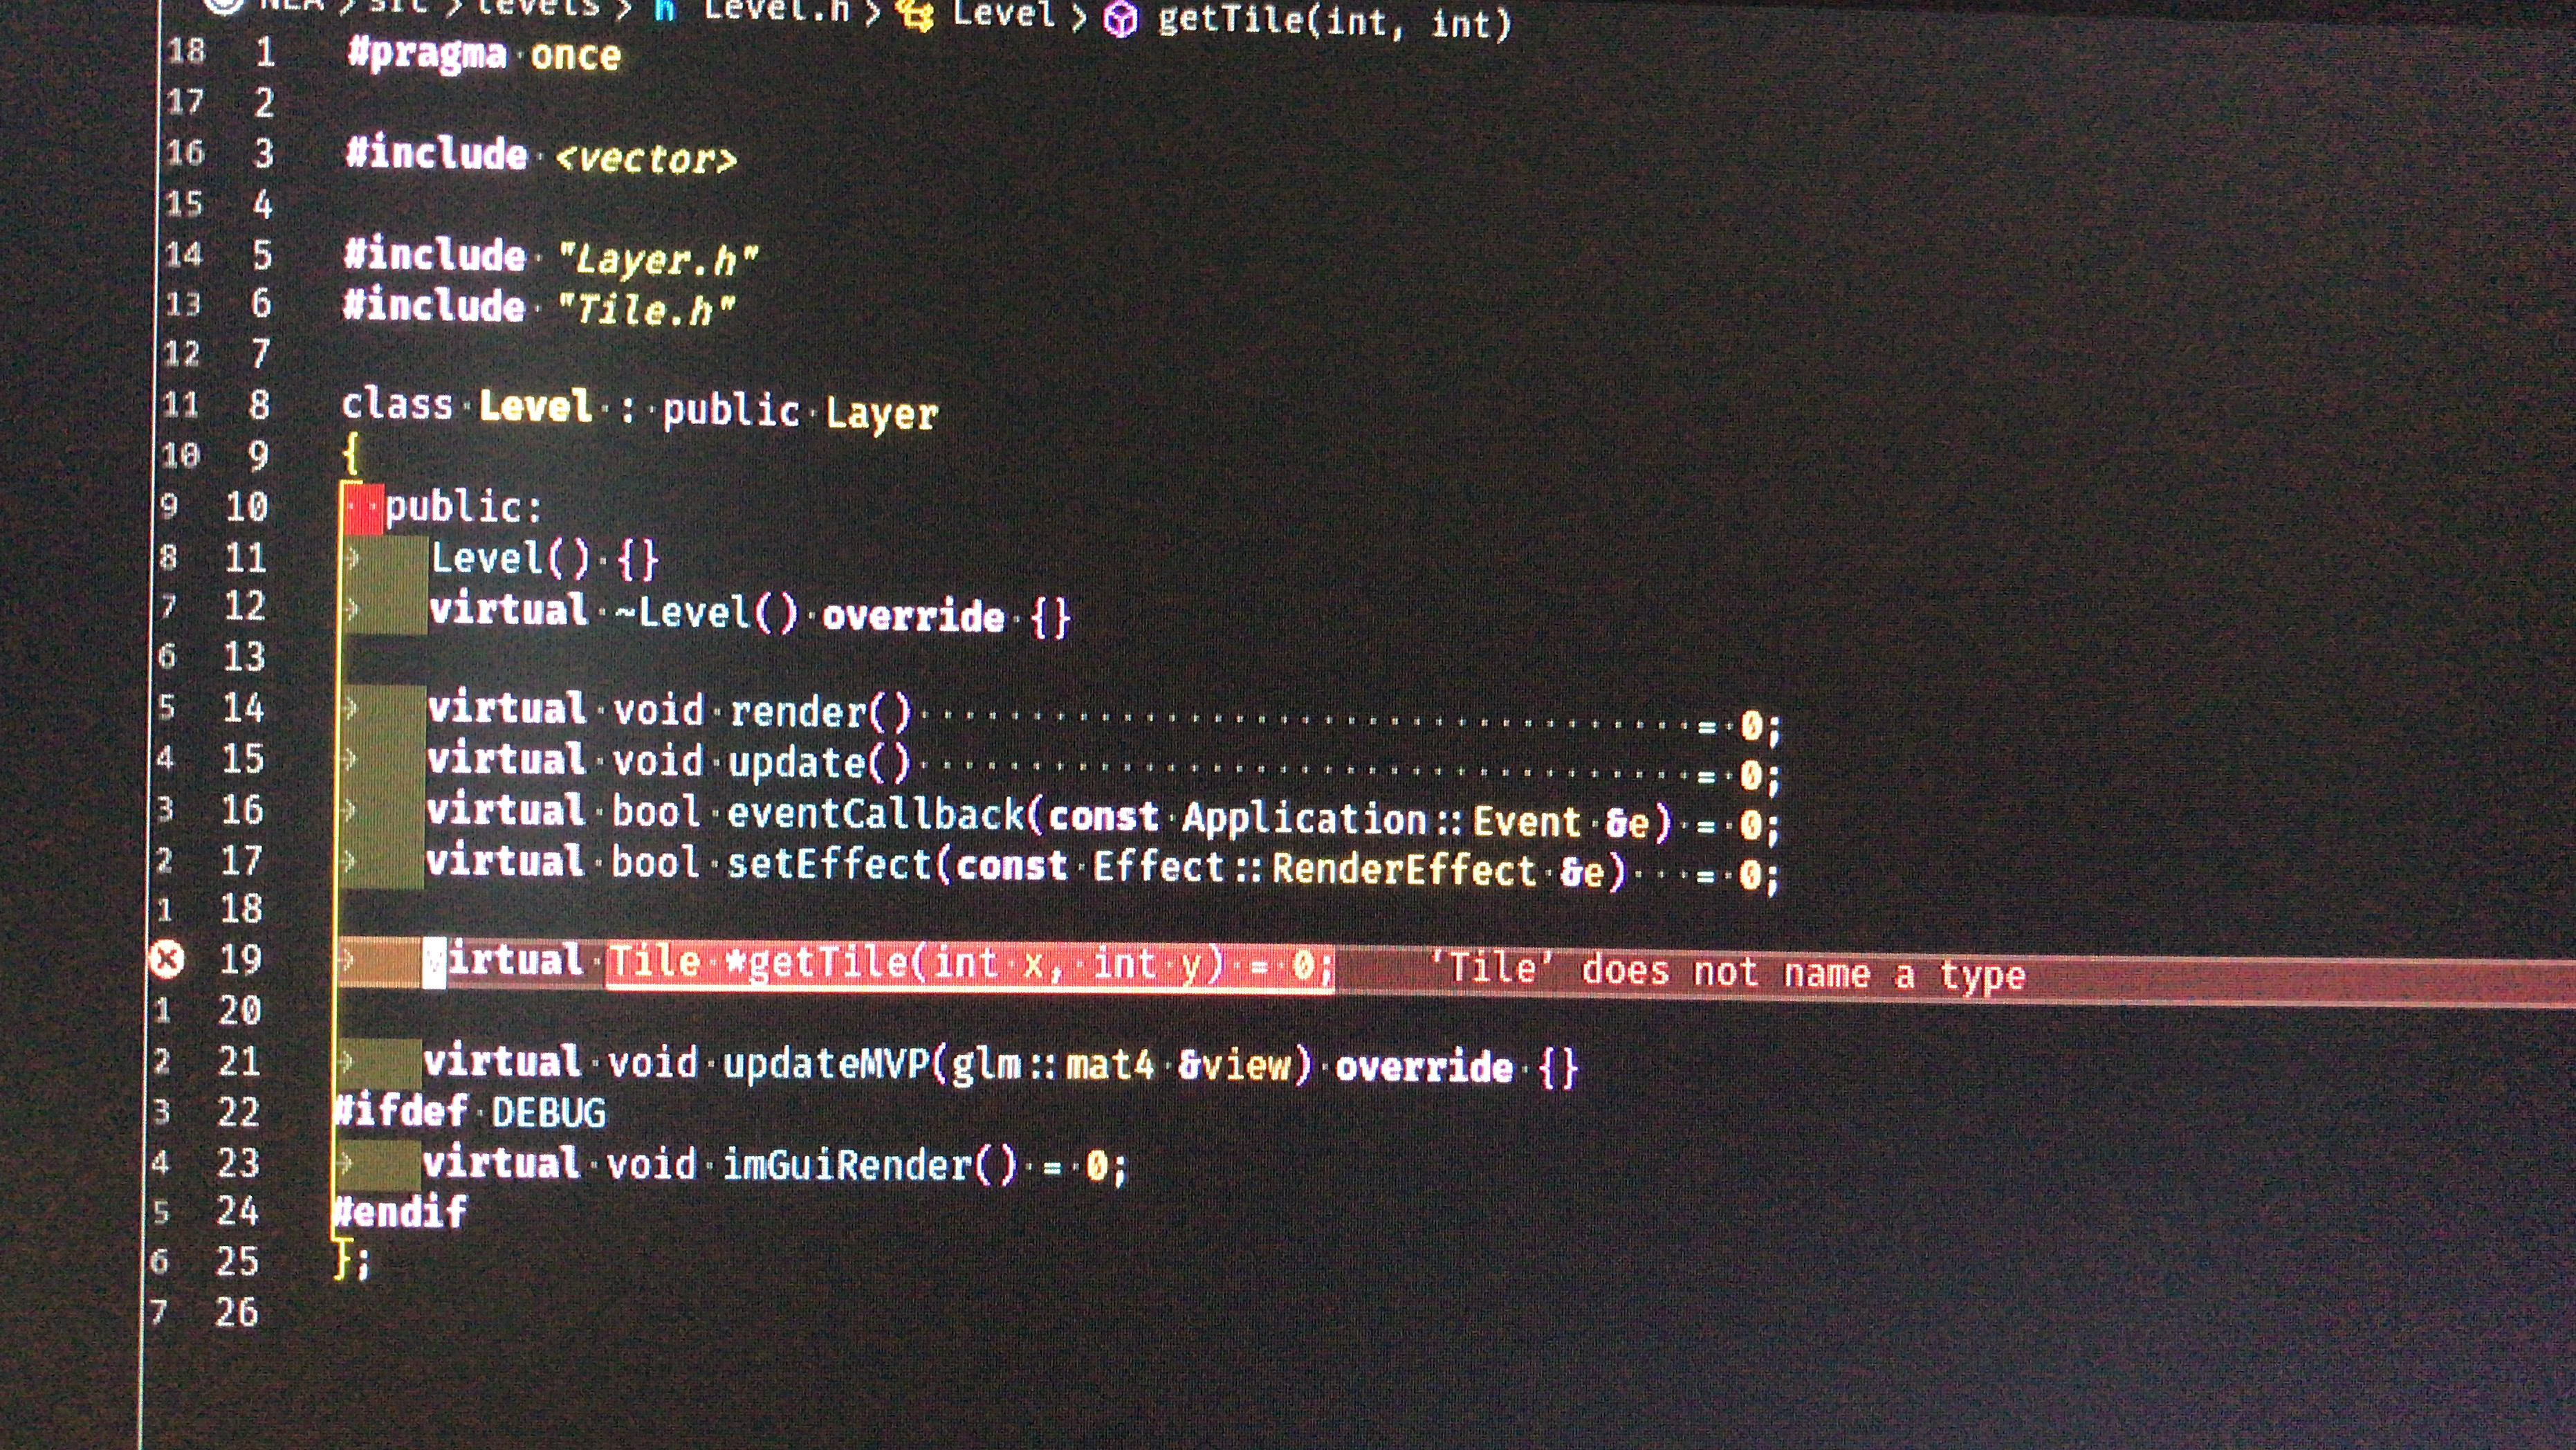
\includegraphics[scale=0.09]{img/Testing/General/Cyclical imports.jpg}}
                \caption{Cyclical imports}
                \label{fig:CyclicalImports1}
            \end{figure}
            \begin{figure}[hbt!]
                \centerline{\includegraphics[scale=0.09]{img/Testing/General/Cyclical imports2.png}}
                \caption{Cyclical imports}
                \label{fig:CyclicalImports2}
            \end{figure}

            As shown in Figures, \ref{fig:CyclicalImports1} (where Tile is included clearly at the top but is not defined) and \ref{fig:CyclicalImports2} (Random errors all over the place), I had a few problems when programming with cyclical imports, where the headers of the file were co-dependent. To fix these issues I had to go through all the header files and clean up the unnecessary includes from them, so that they would only include the files that they absolutely needed. which fixed the issues.
    \clearpage
    \subsection{Objective Testing}
        These tests were performed to test that all the objectives were met.
        \subsubsection{Figures}
            \begin{figure}[hbt!]
                \centerline{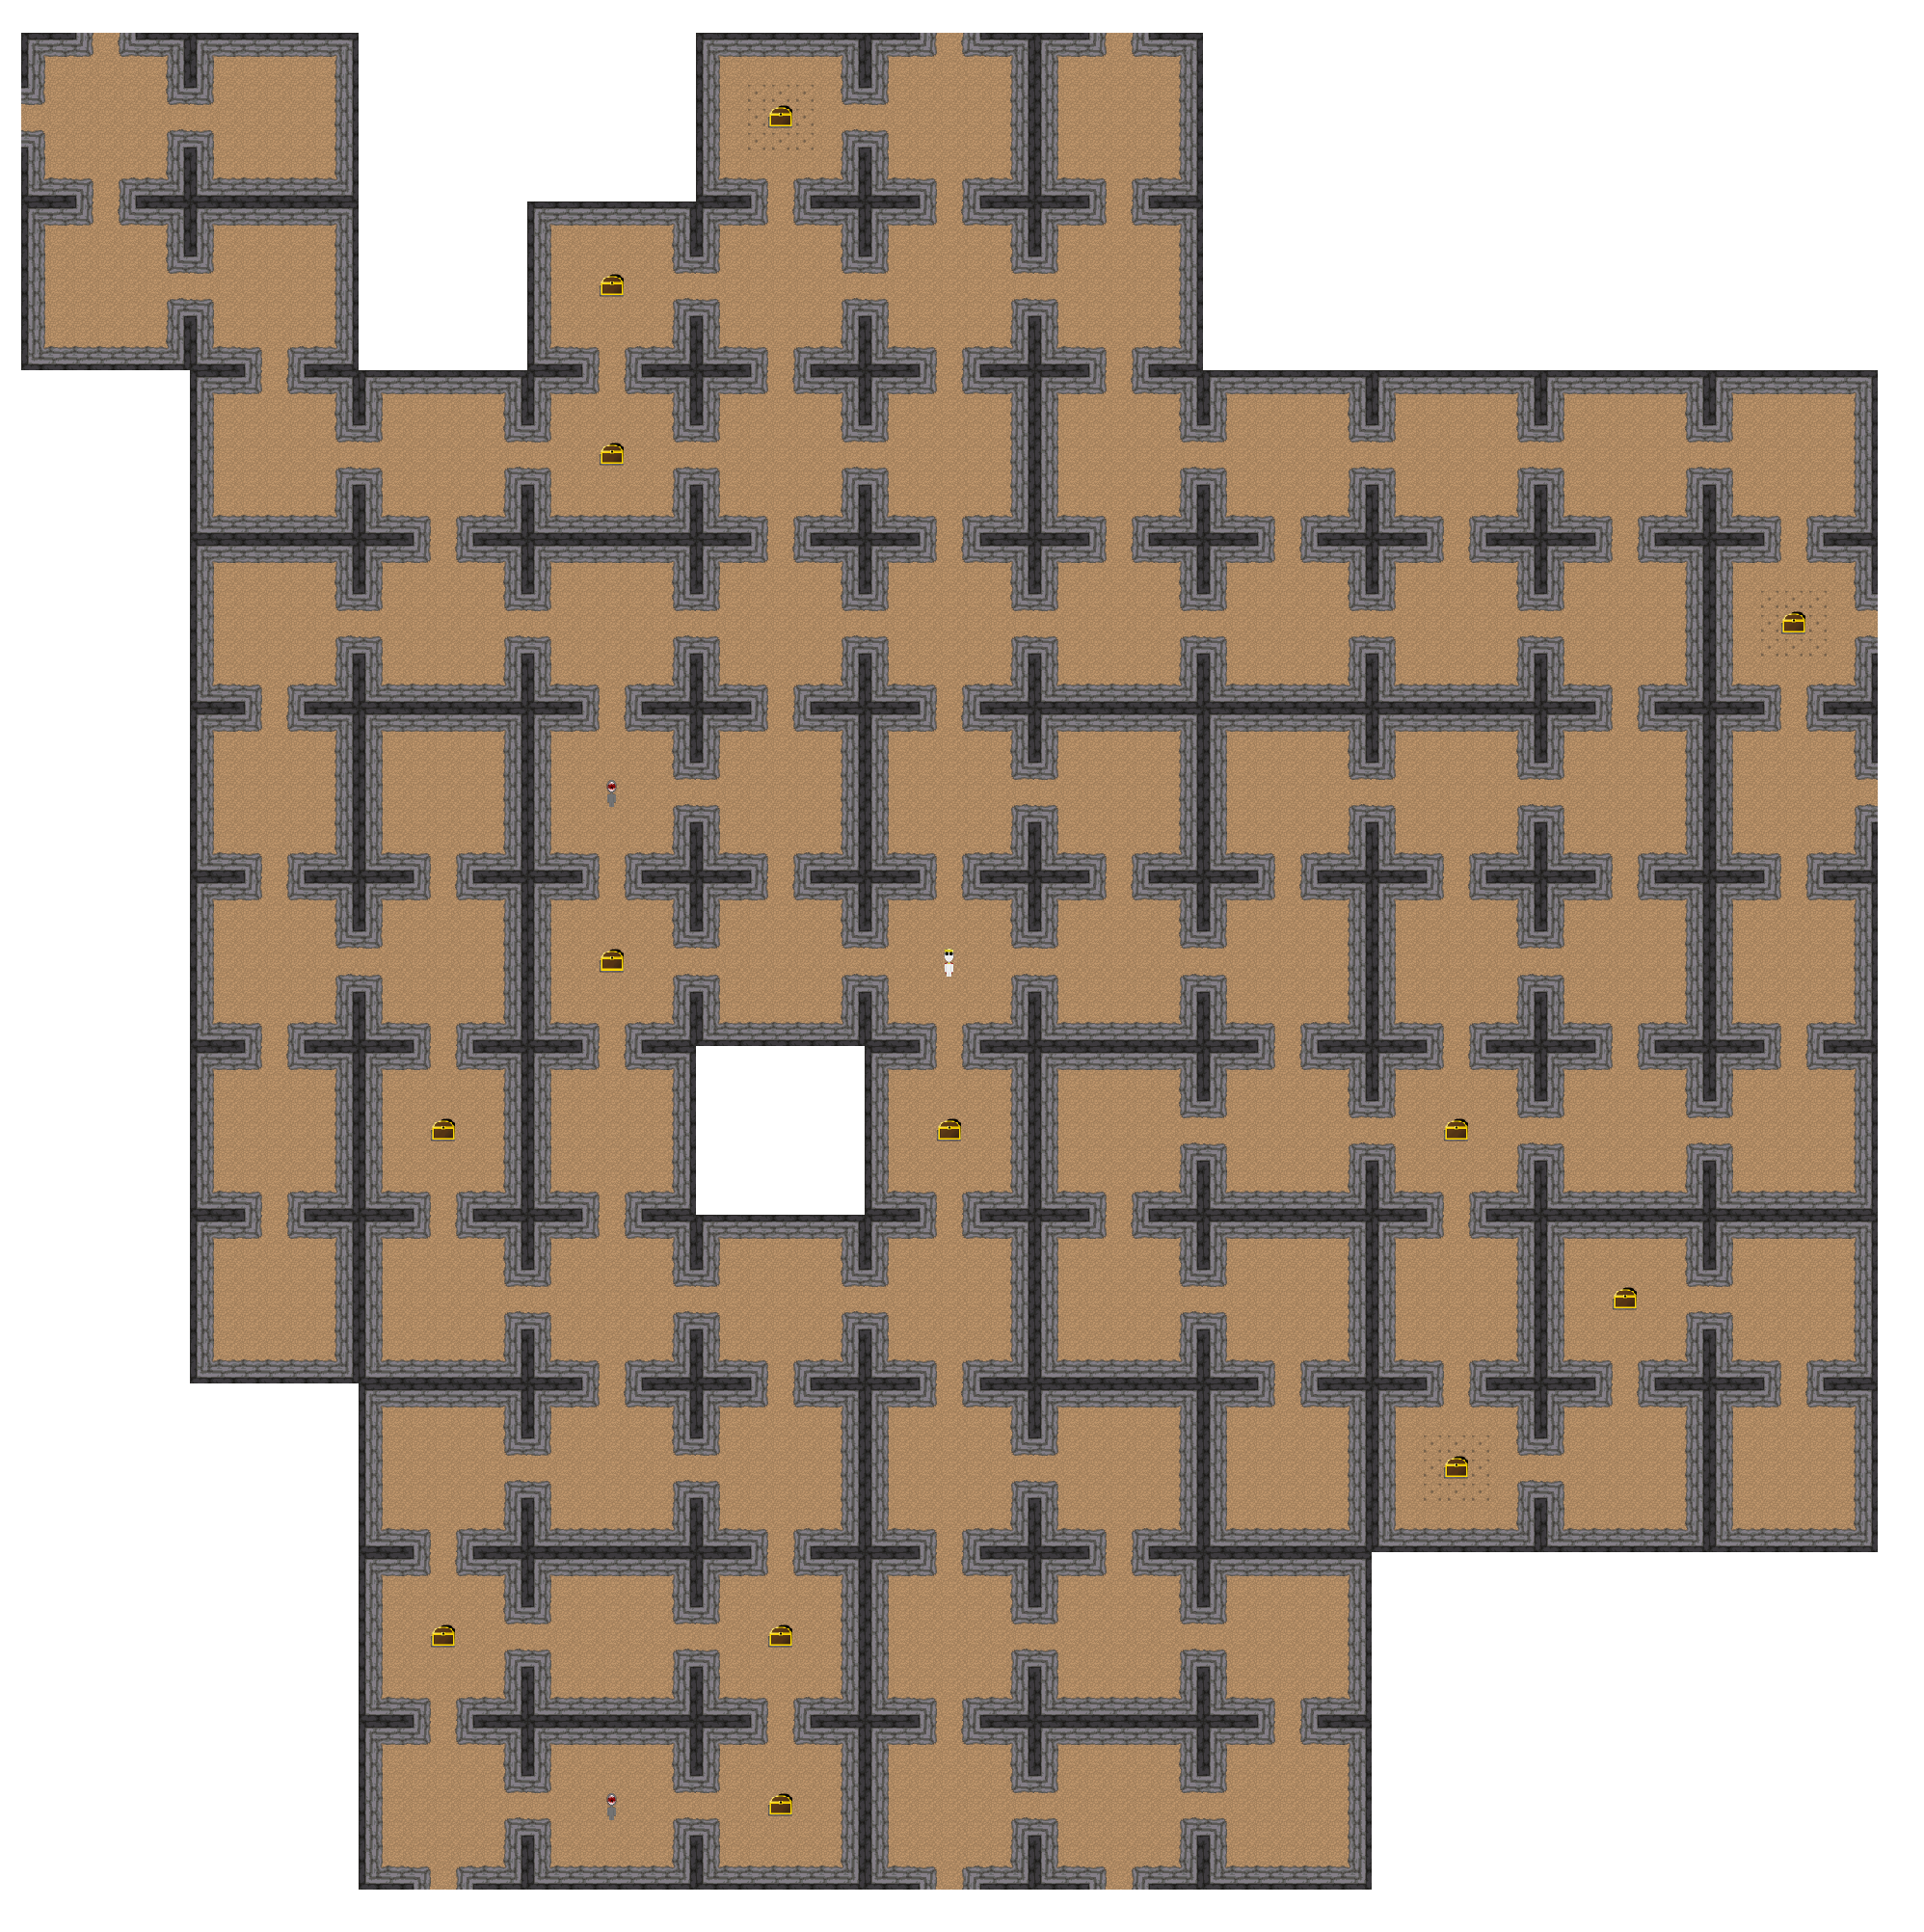
\includegraphics[scale=0.4]{img/Testing/Objective/Full Maze.png}}
                \caption{All of the maze when generated}
                \label{fig:FullMaze}
            \end{figure}
            \begin{figure}[hbt!]
                \centerline{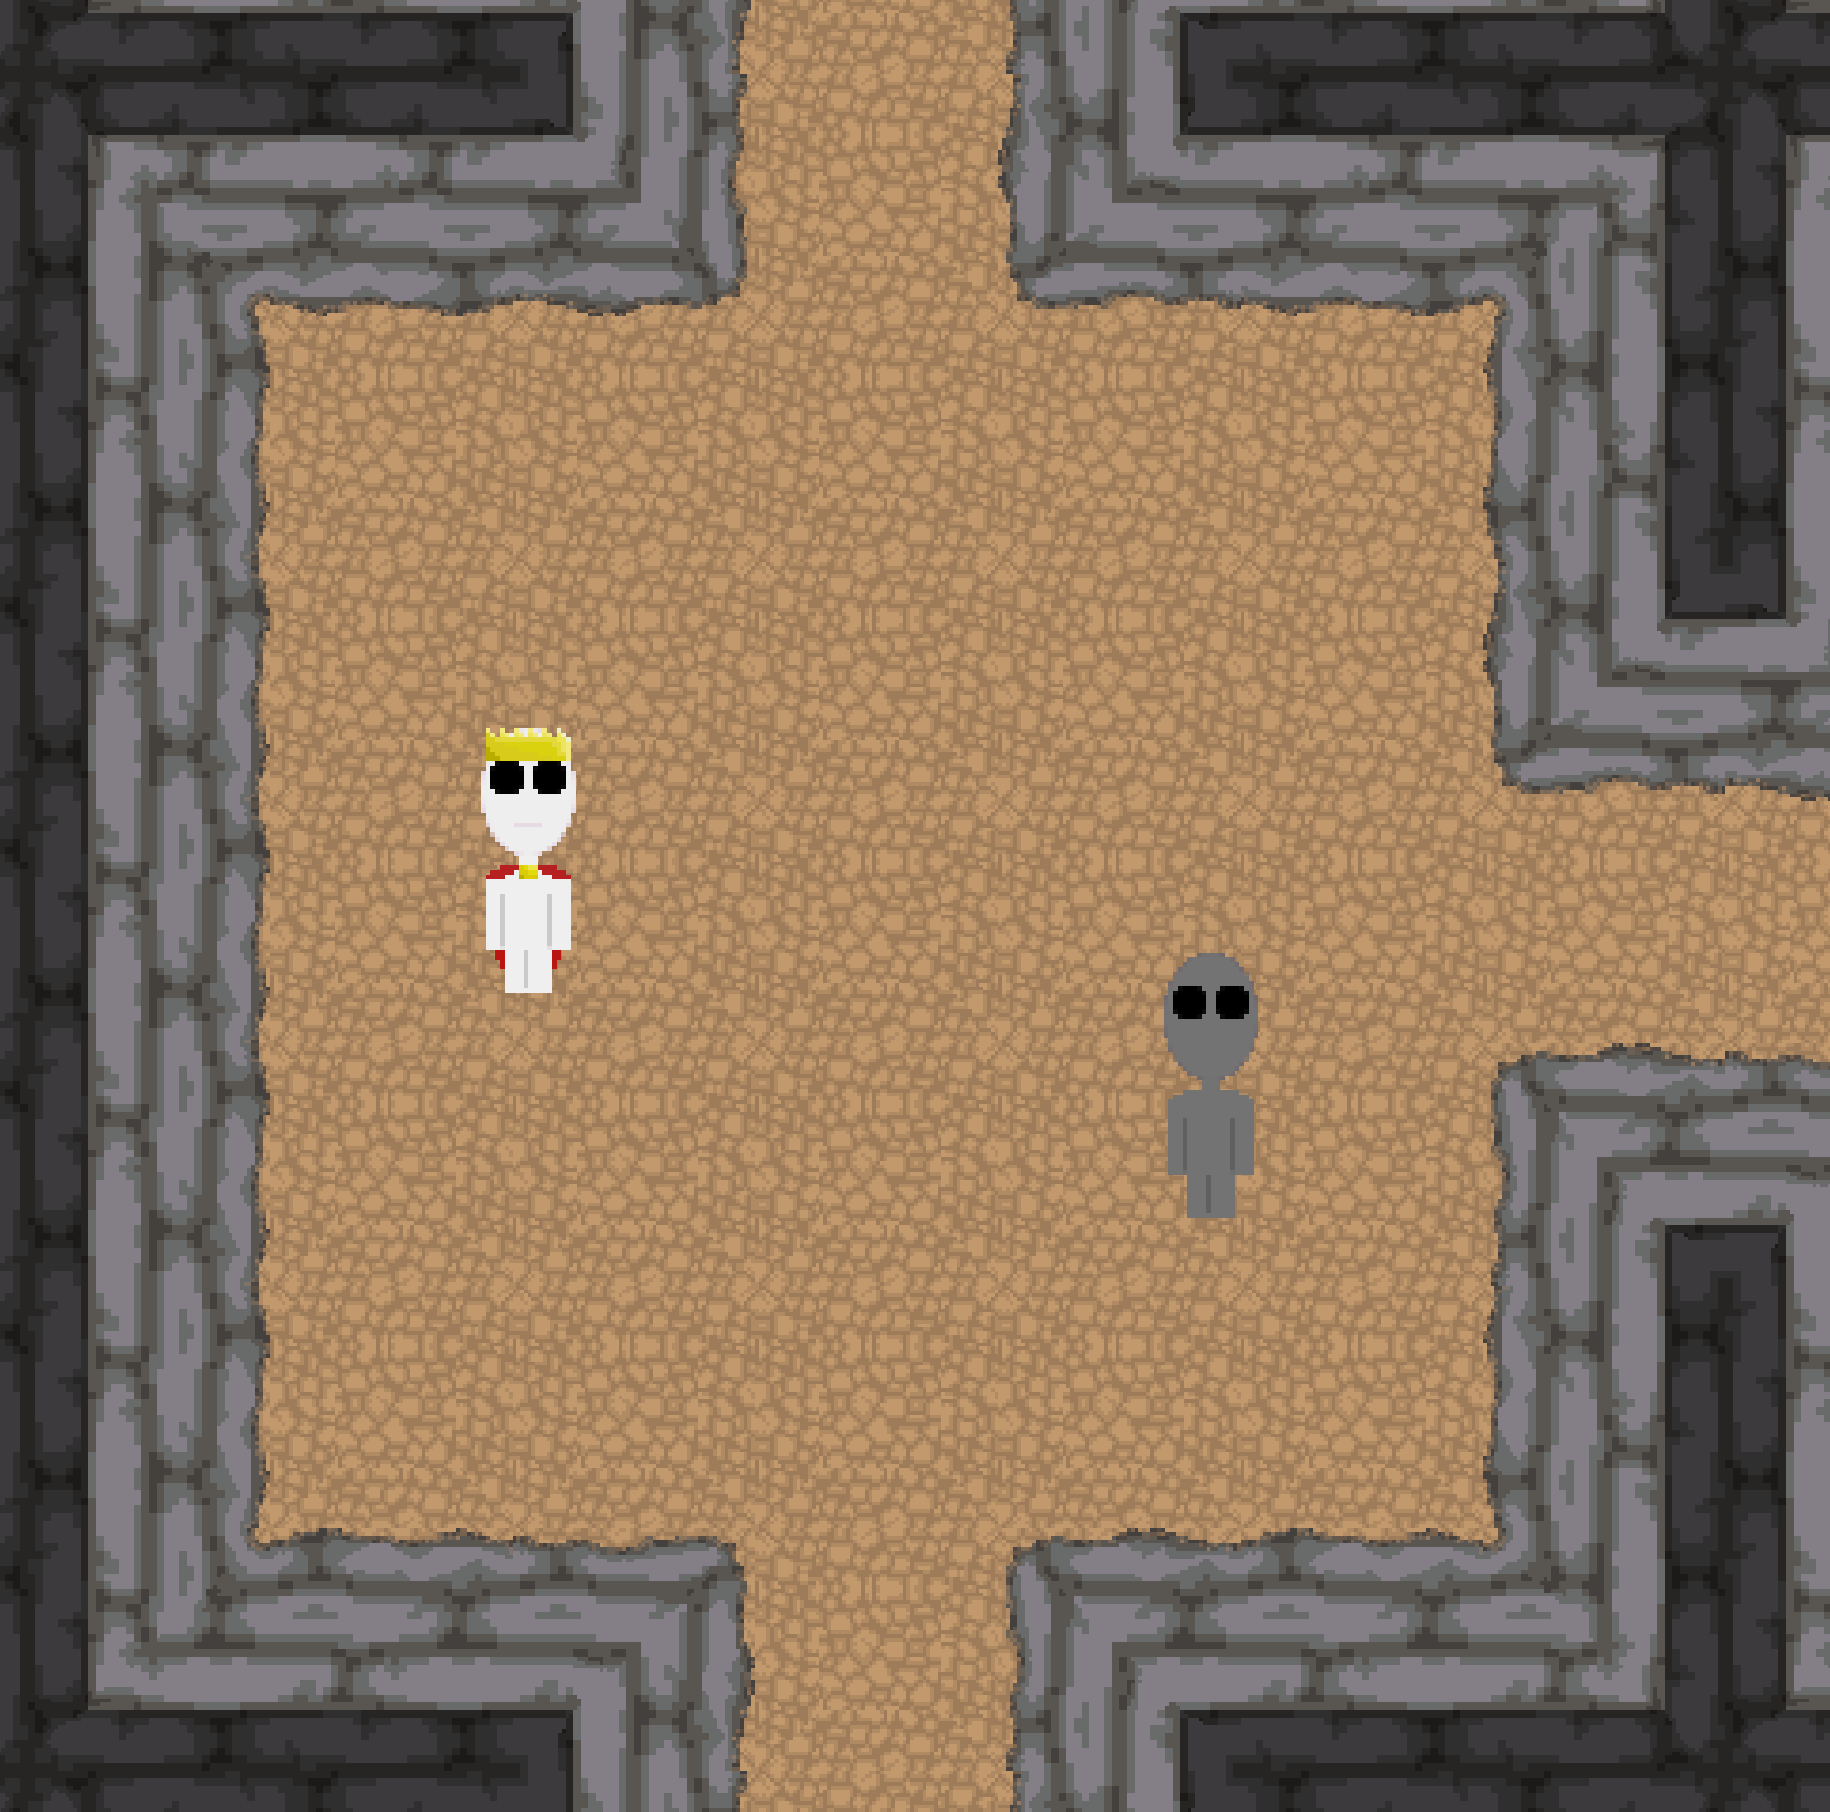
\includegraphics[scale=0.4]{img/Testing/Objective/Follower.png}}
                \caption{Follower}
                \label{fig:Follower}
            \end{figure}
            \begin{figure}[hbt!]
                \centerline{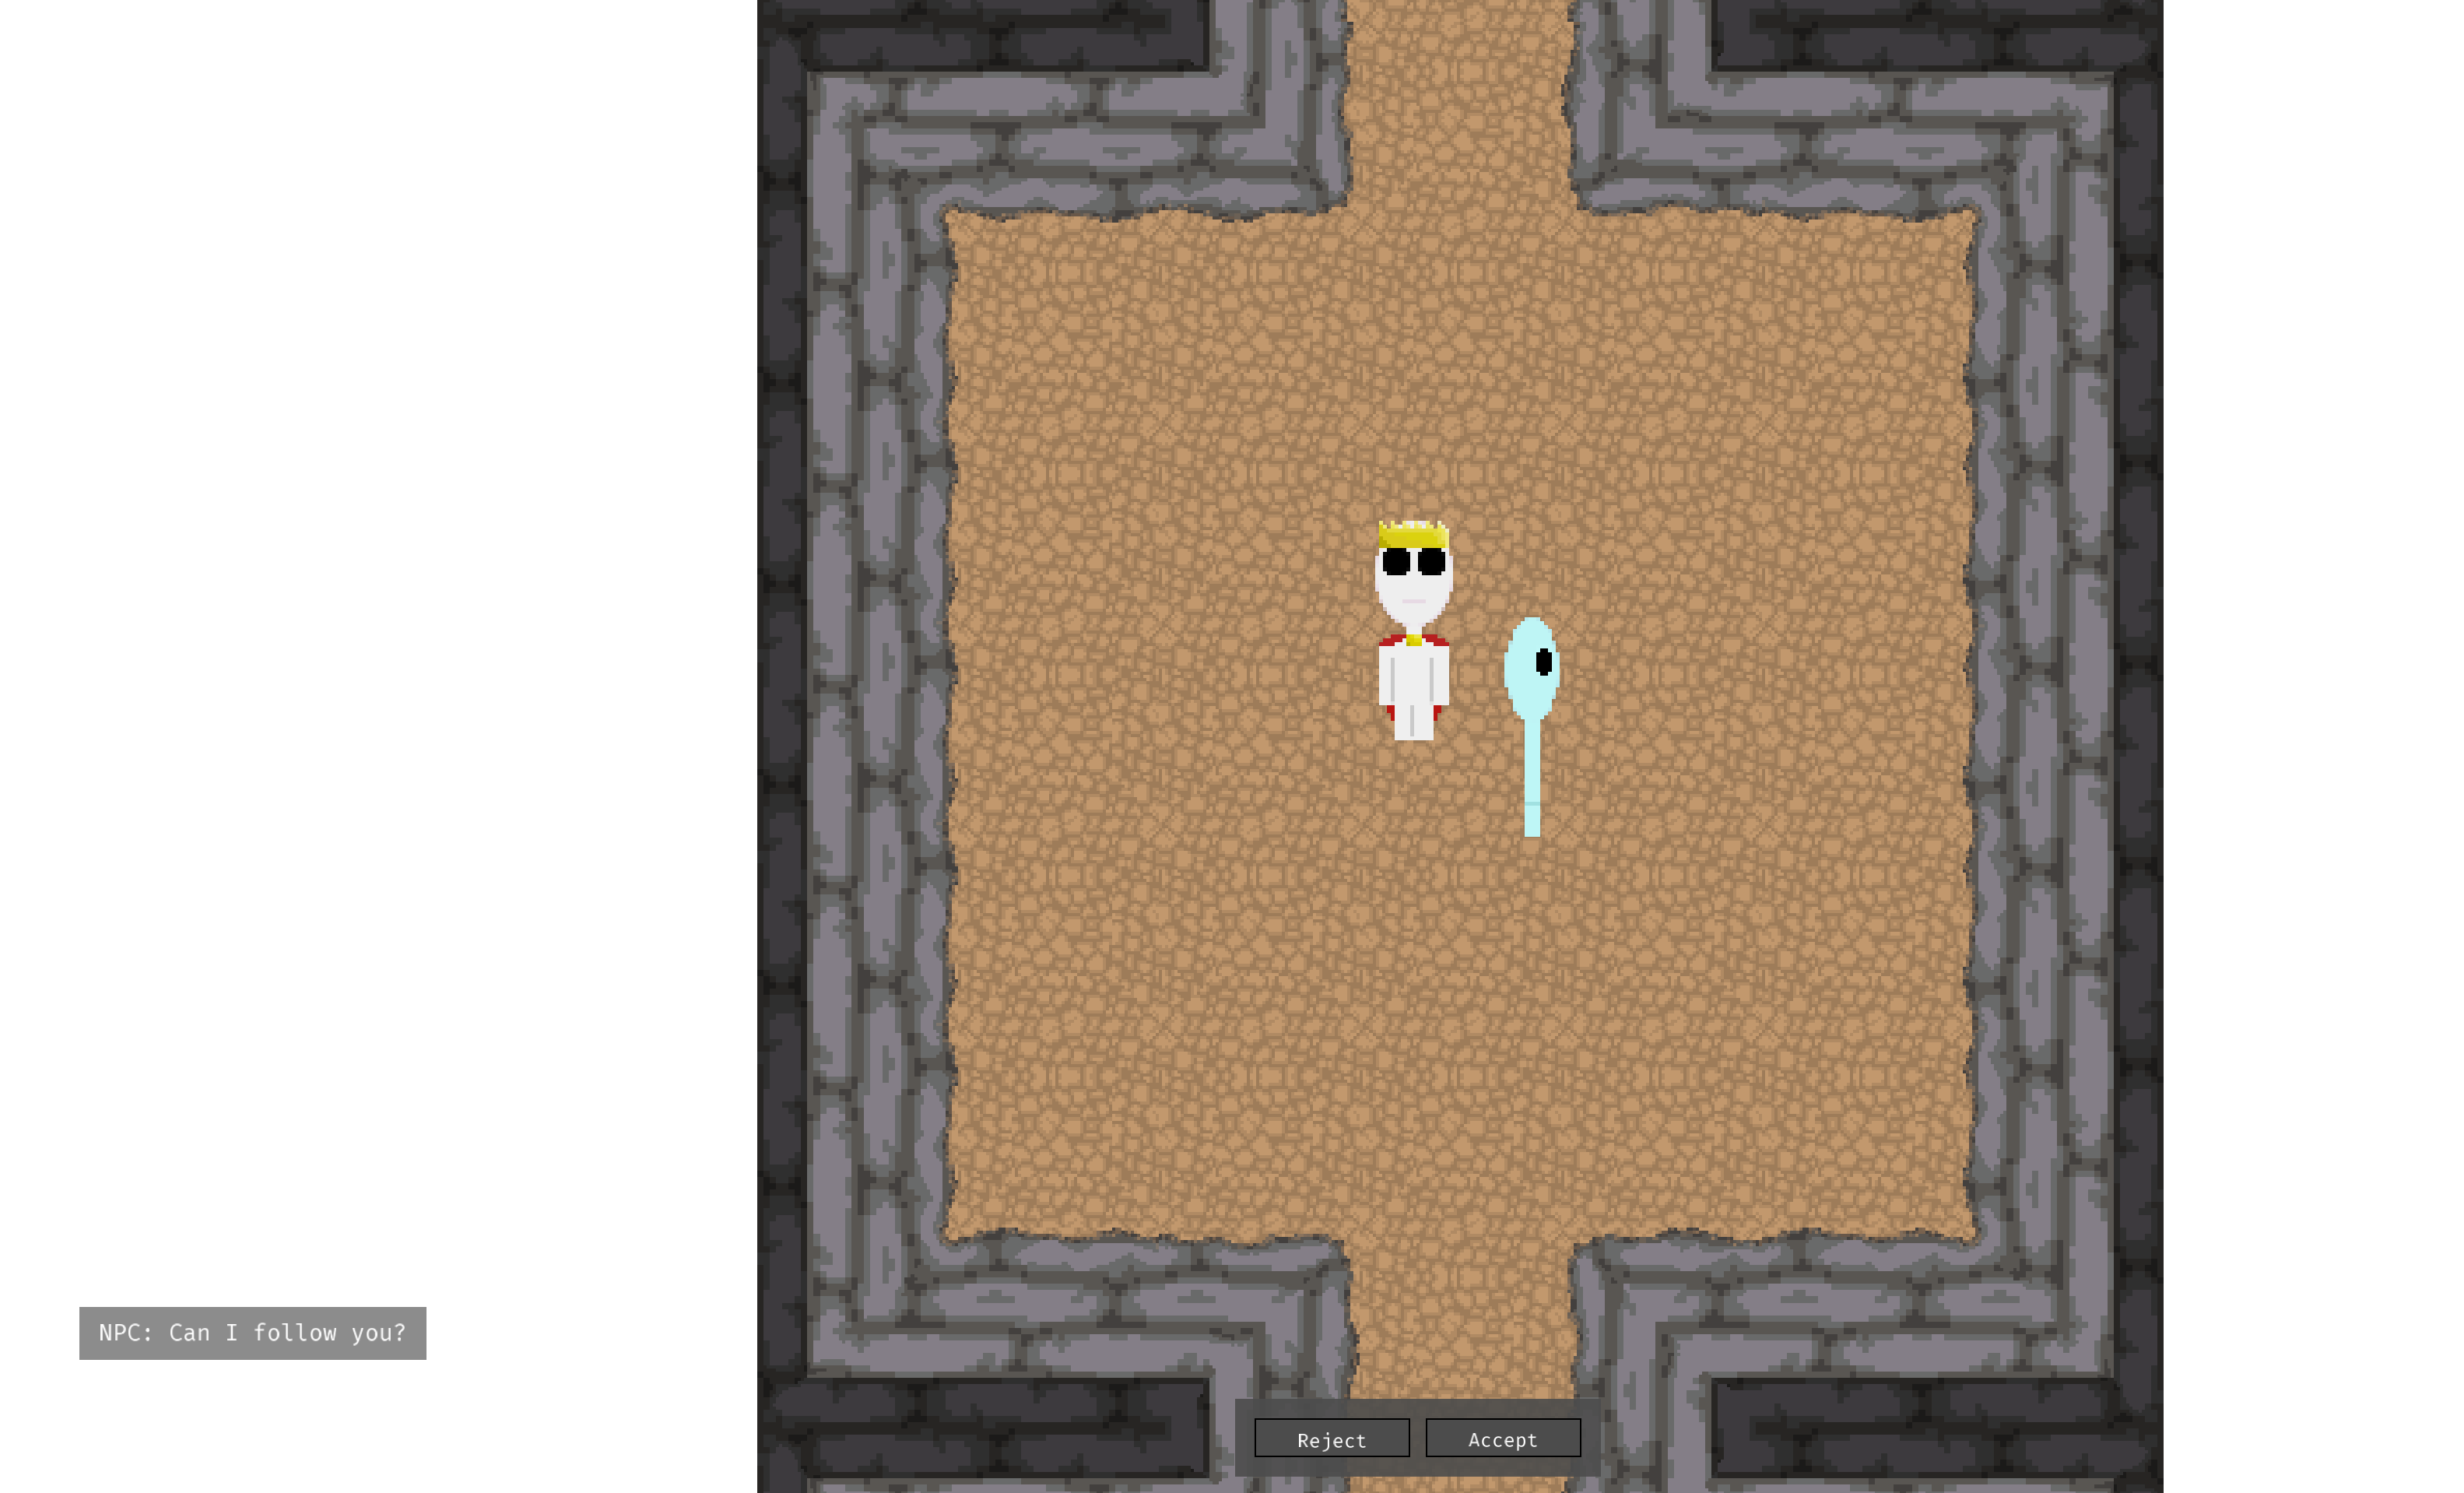
\includegraphics[scale=0.4]{img/Testing/Objective/FollowerQuestion.png}}
                \caption{After clicking on the follower, you can choose to allow them to follow you}
                \label{fig:FollowerQuestion}
            \end{figure}
            \begin{figure}[hbt!]
                \centerline{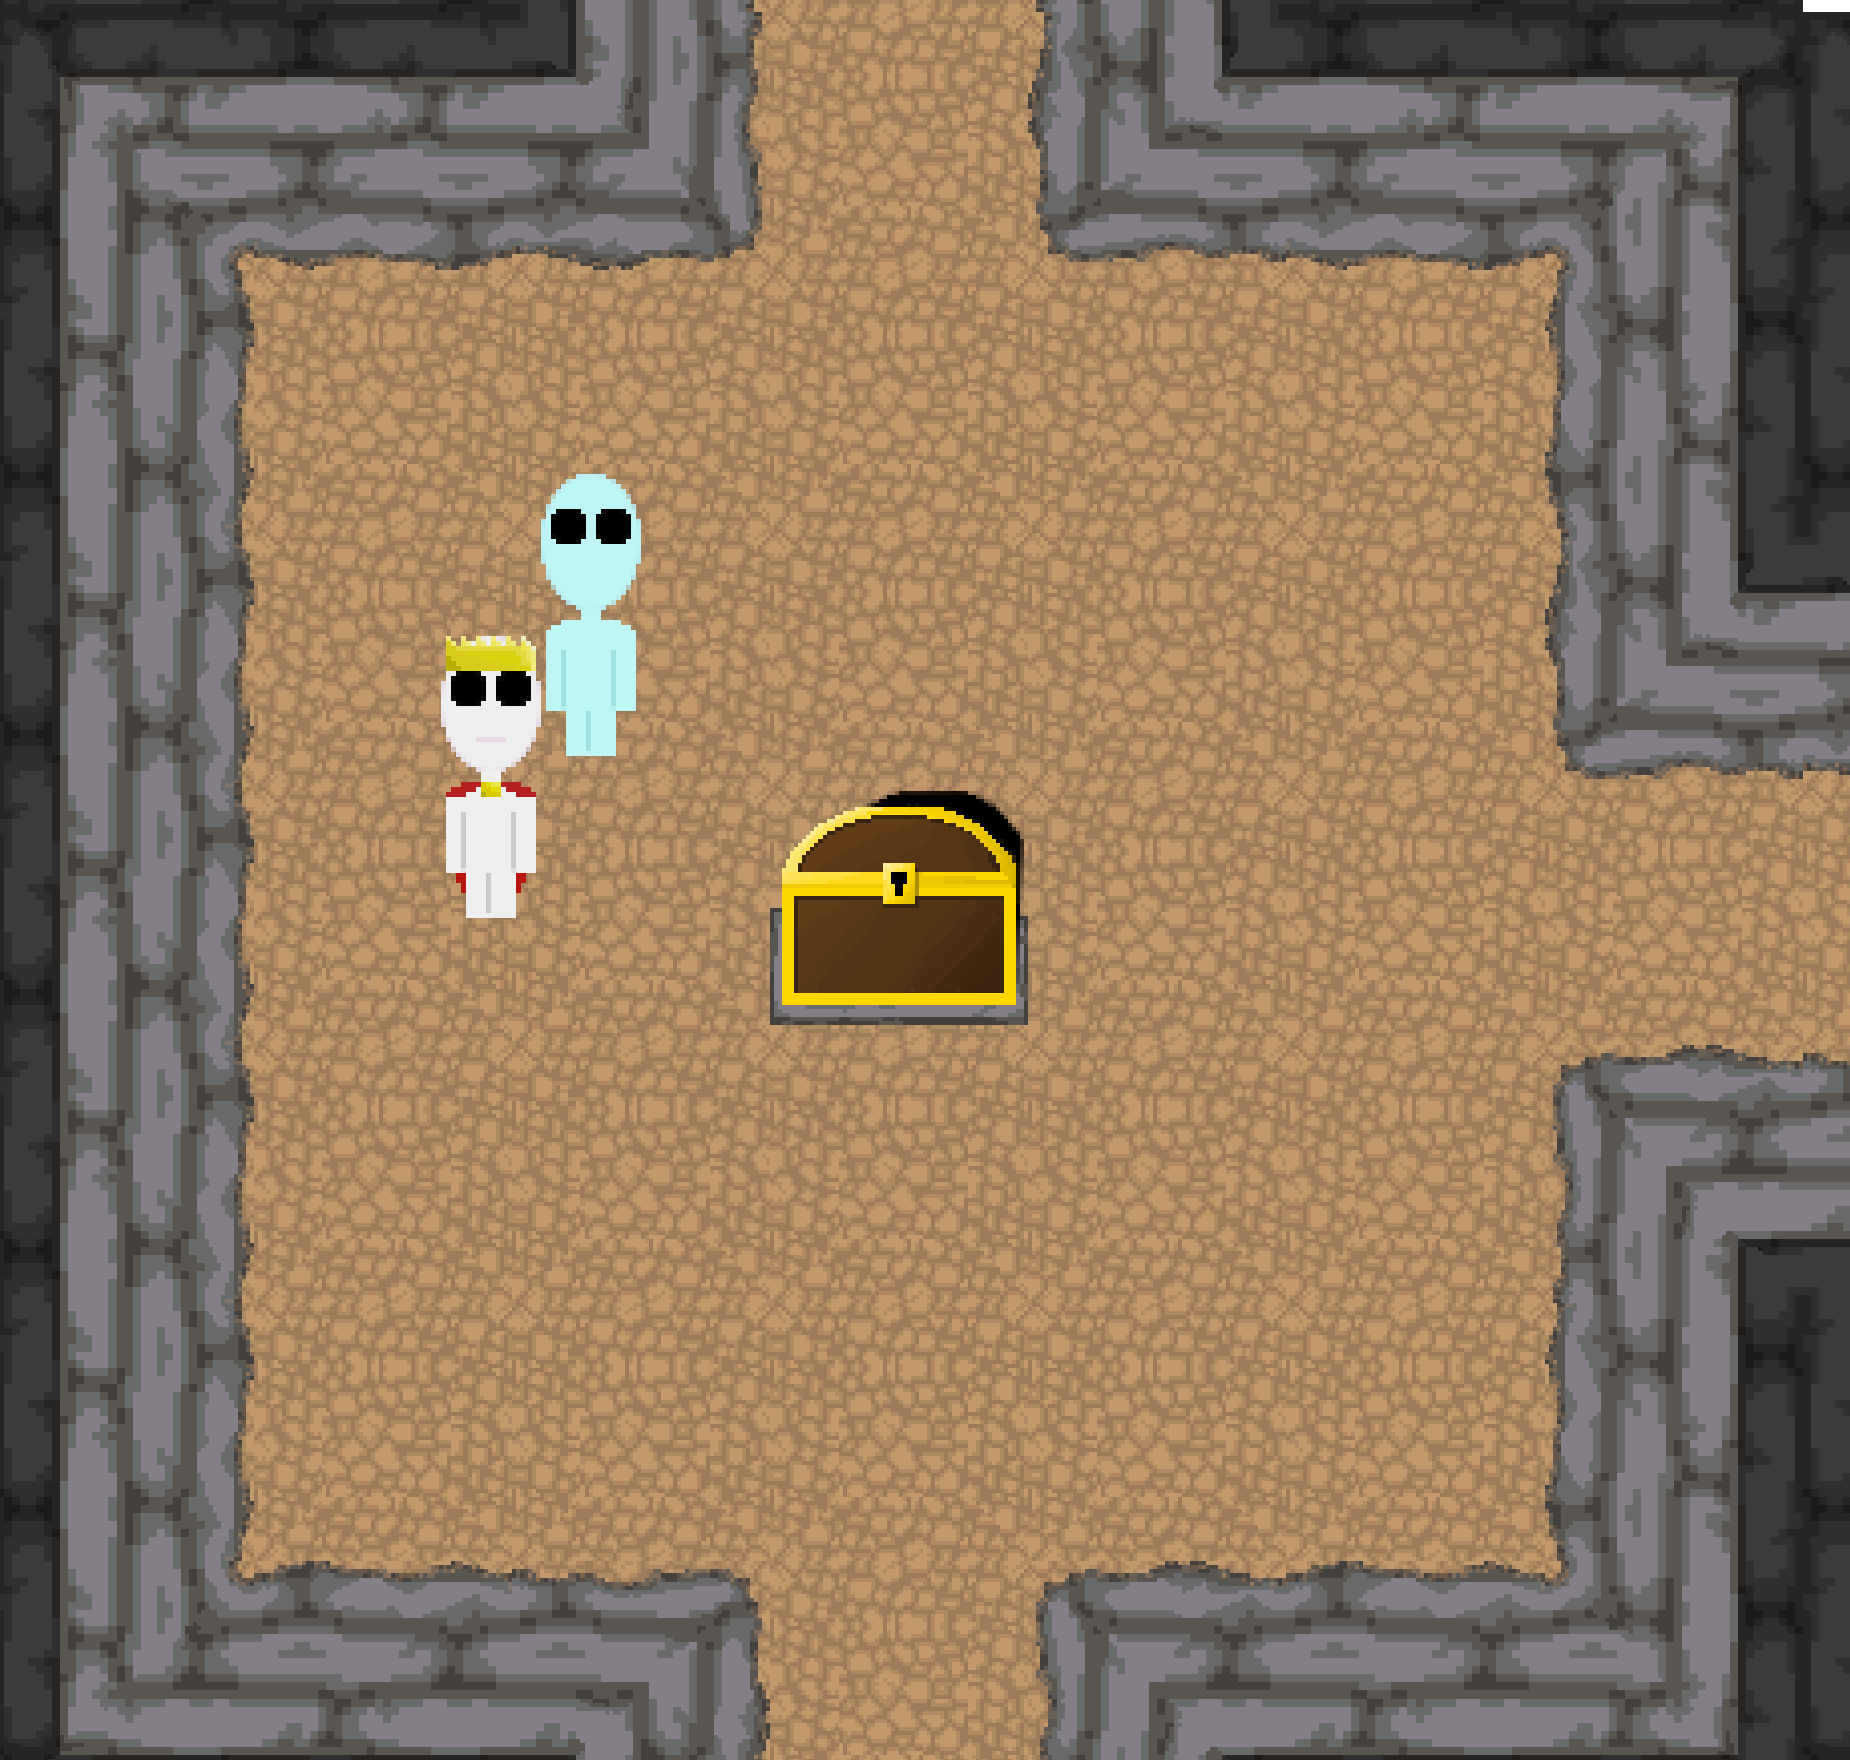
\includegraphics[scale=0.4]{img/Testing/Objective/FollowerFollowing.png}}
                \caption{A follower following the player using the A* algorithm}
                \label{fig:FollowerFollowing}
            \end{figure}
            \begin{figure}[hbt!]
                \centerline{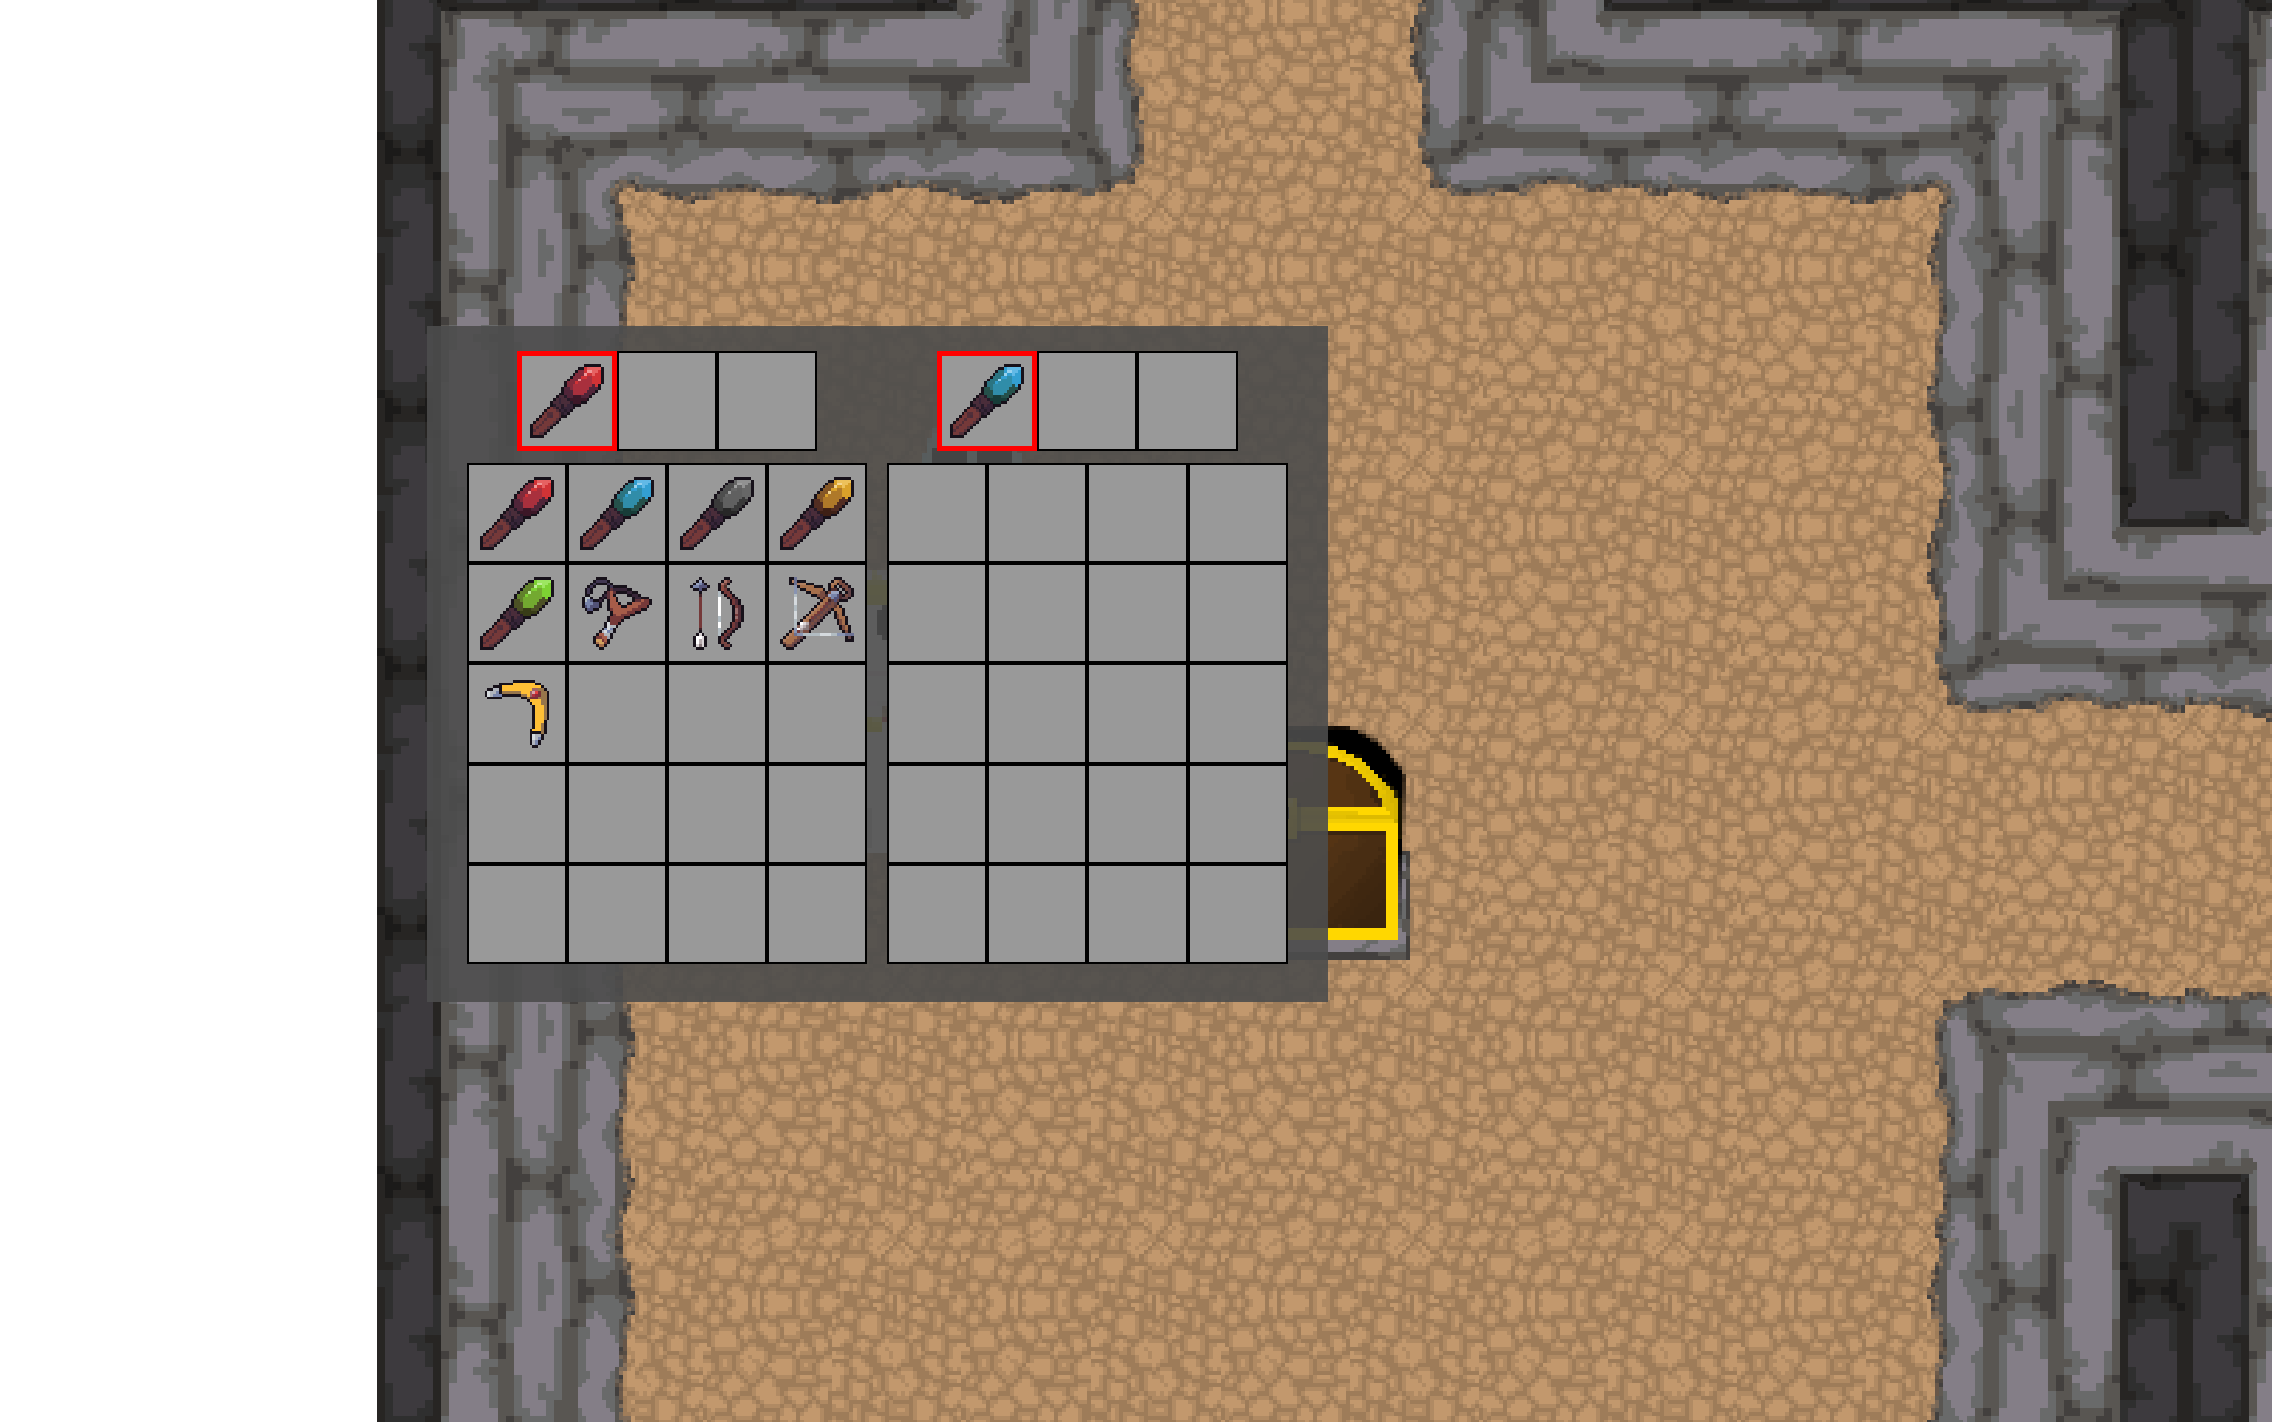
\includegraphics[scale=0.4]{img/Testing/Objective/FollowerInventory.png}}
                \caption{Clicking on a follower results in their inventory popping up, which you can then change}
                \label{fig:FollowerInventory}
            \end{figure}
            \begin{figure}[hbt!]
                \centerline{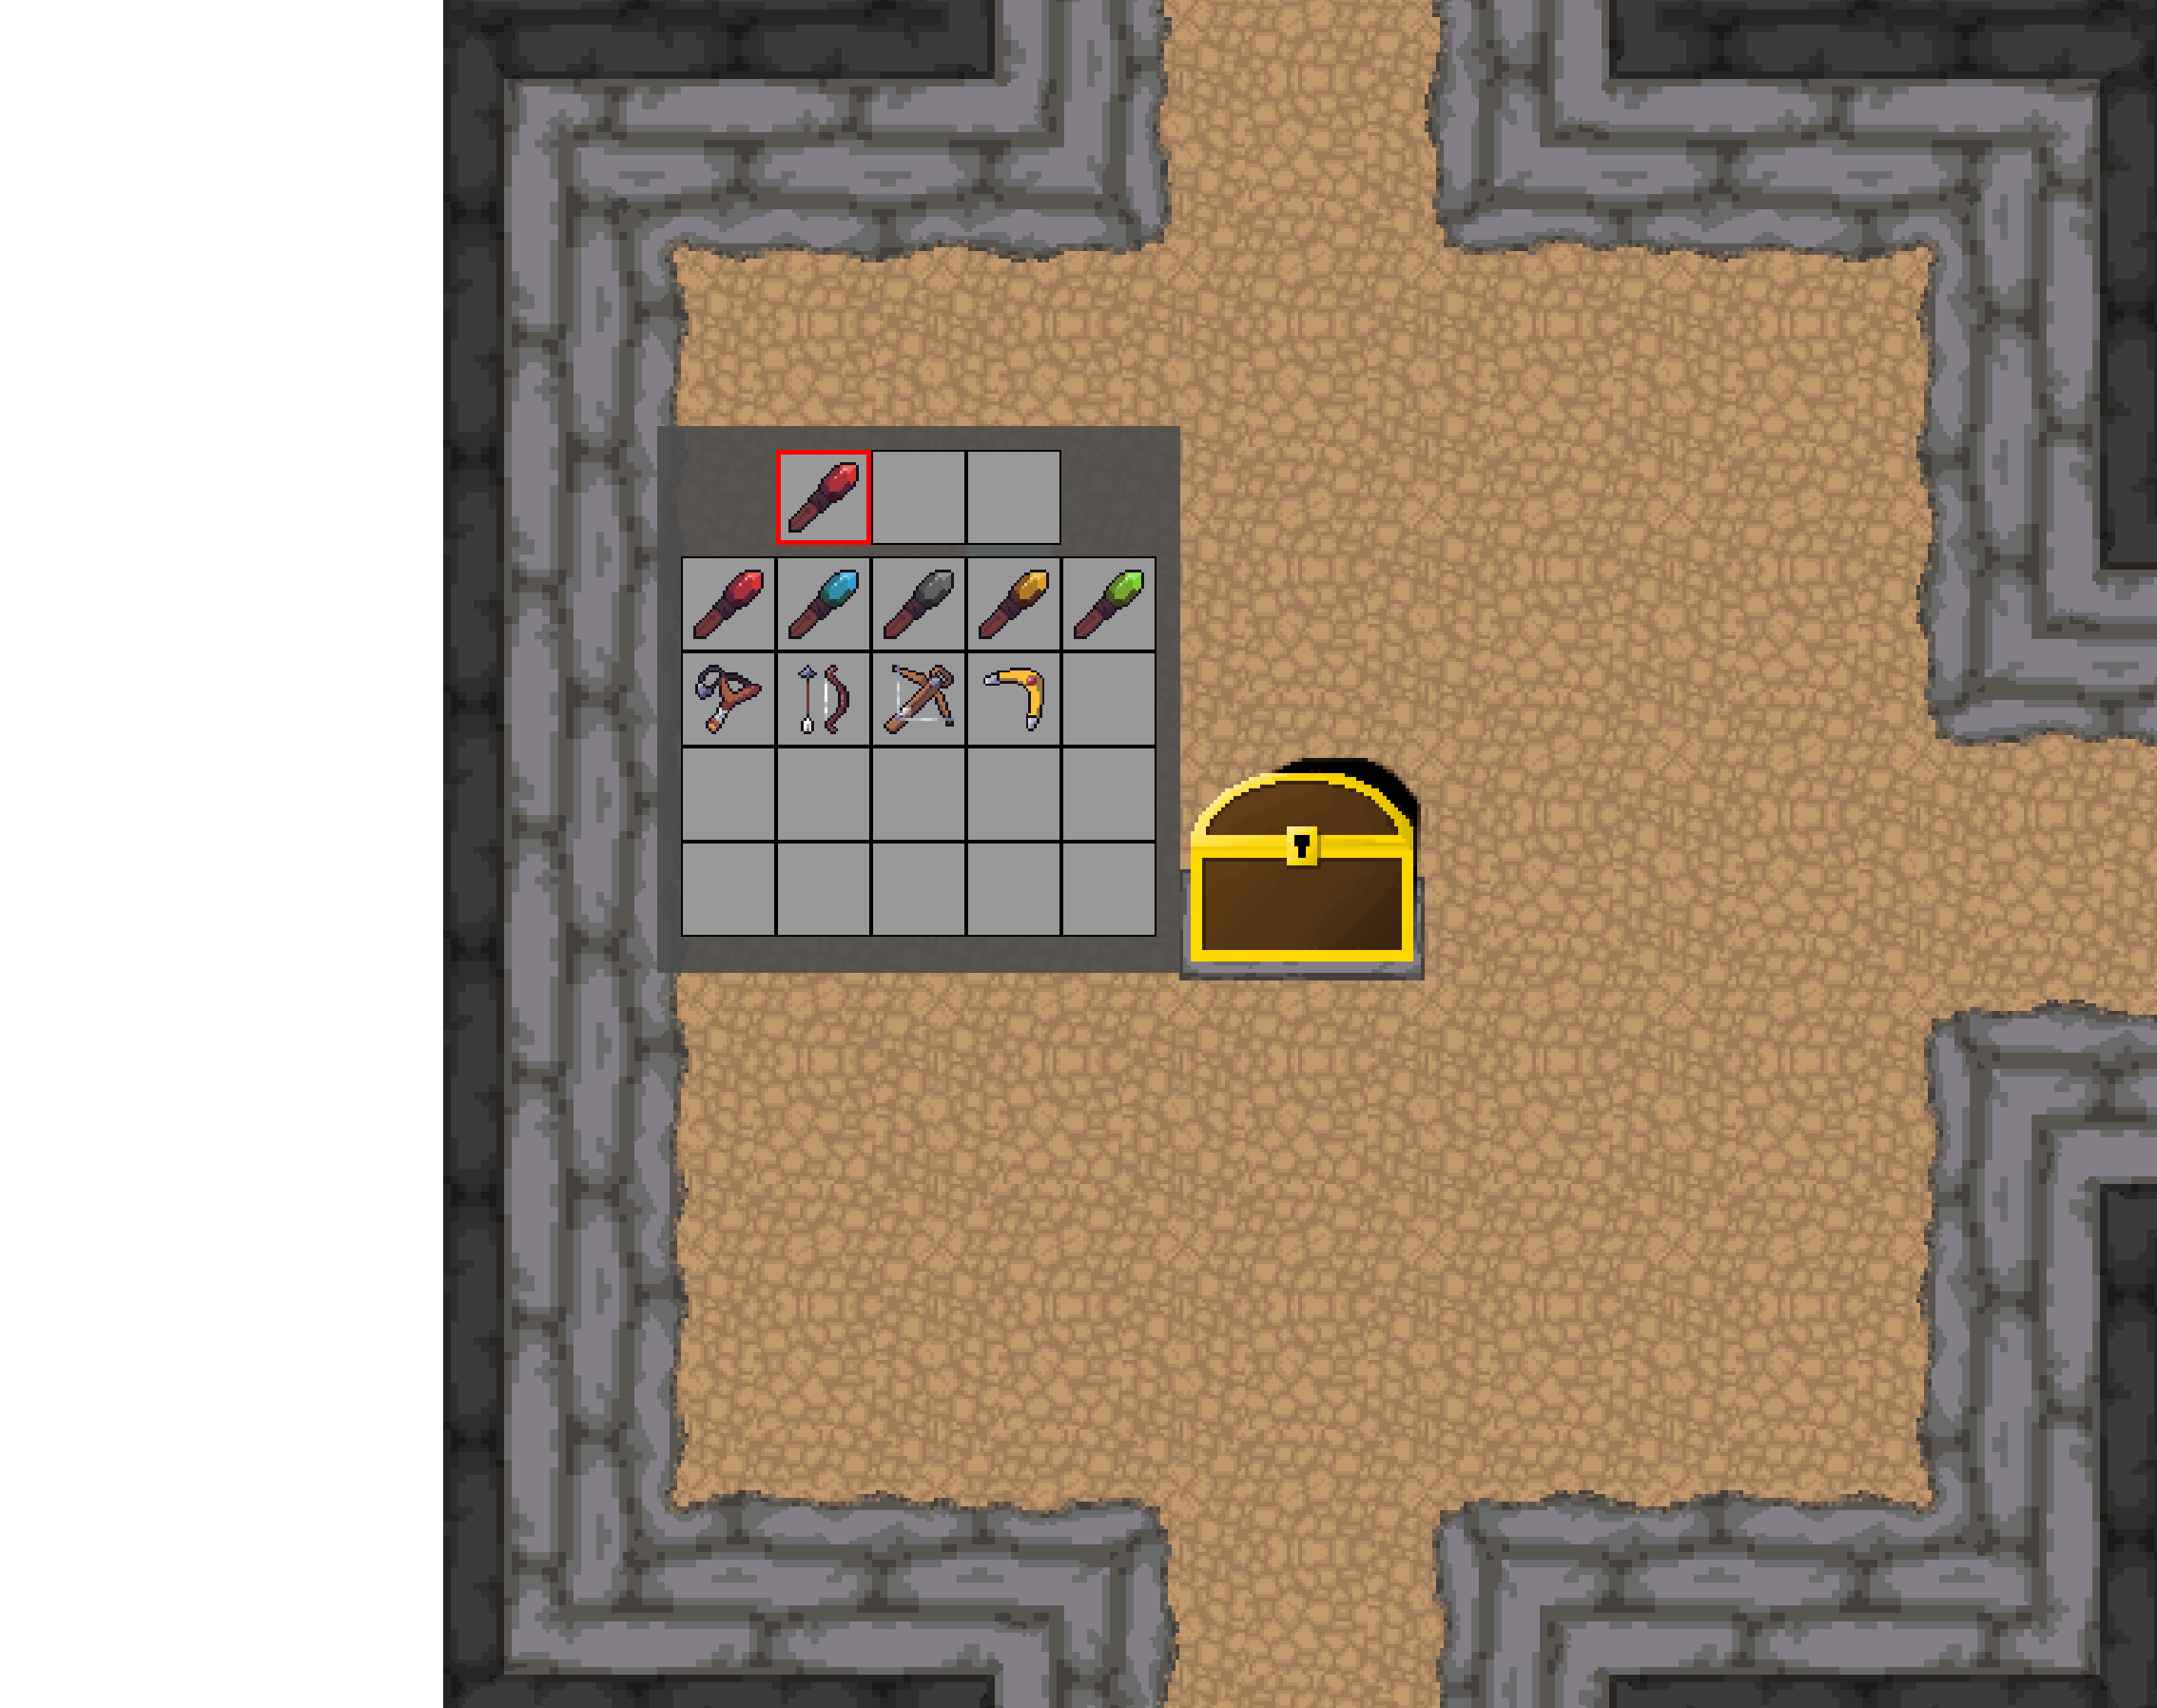
\includegraphics[scale=0.4]{img/Testing/Objective/PlayerInventory.png}}
                \caption{Player inventory with all the weapons in the game}
                \label{fig:PlayerInventory}
            \end{figure}
            \begin{figure}[hbt!]
                \centerline{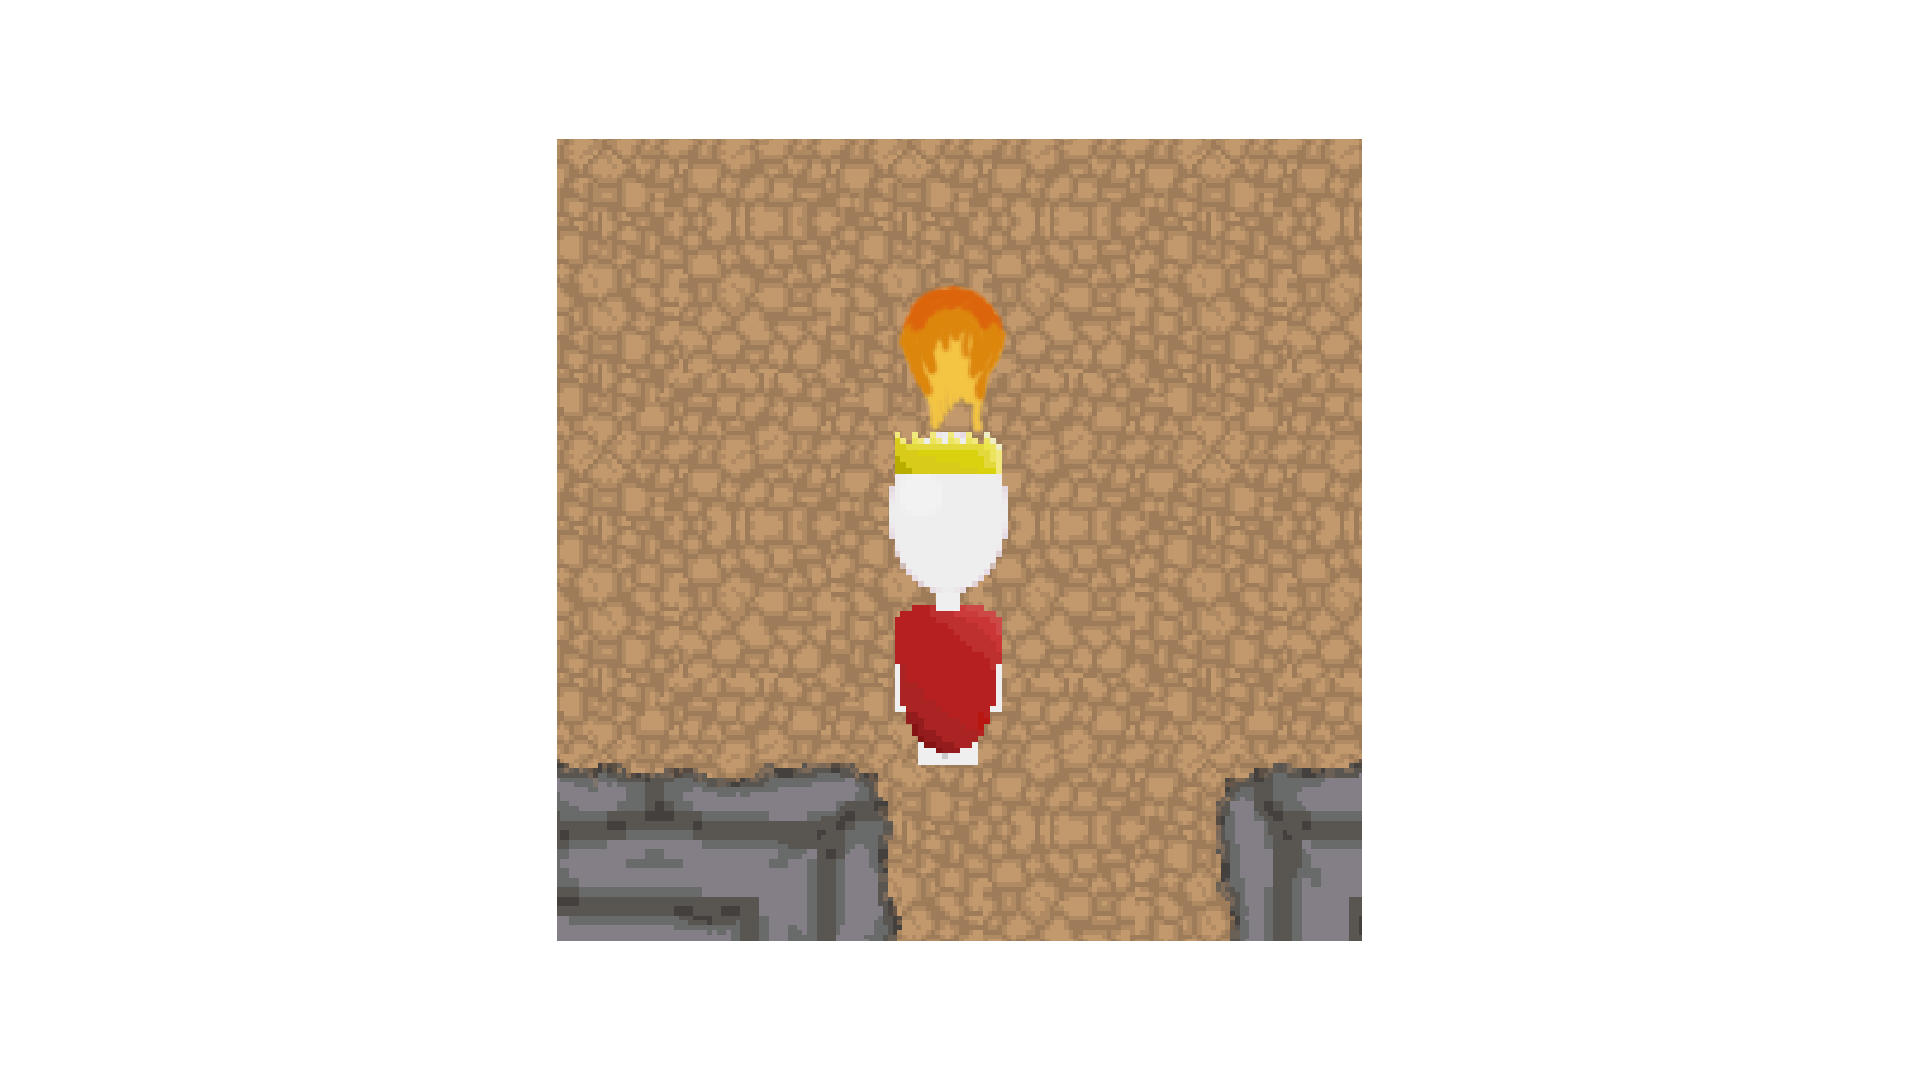
\includegraphics[scale=0.7]{img/Testing/Objective/Firing.png}}
                \caption{The player can fire projectiles when they have gained a weapon}
                \label{fig:Firing}
            \end{figure}
            \begin{figure}[hbt!]
                \centerline{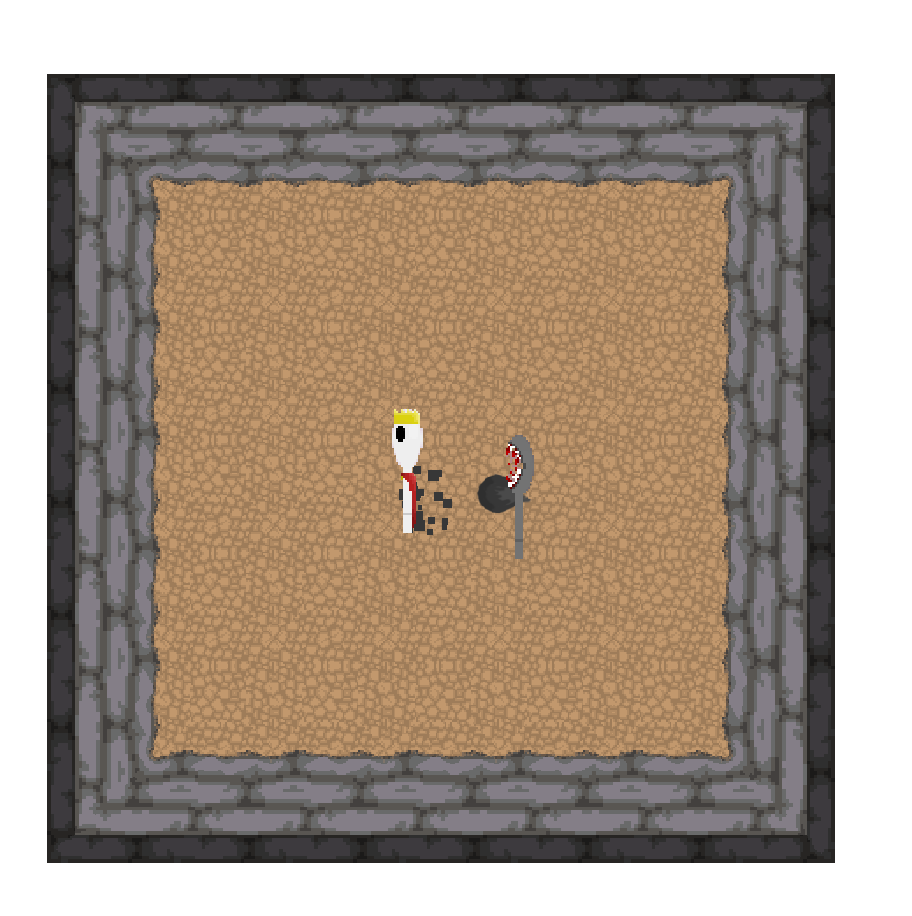
\includegraphics[scale=0.6]{img/Testing/Objective/Enemy.png}}
                \caption{Enemy attacking the player}
                \label{fig:Enemy}
            \end{figure}
            \begin{figure}[hbt!]
                \centerline{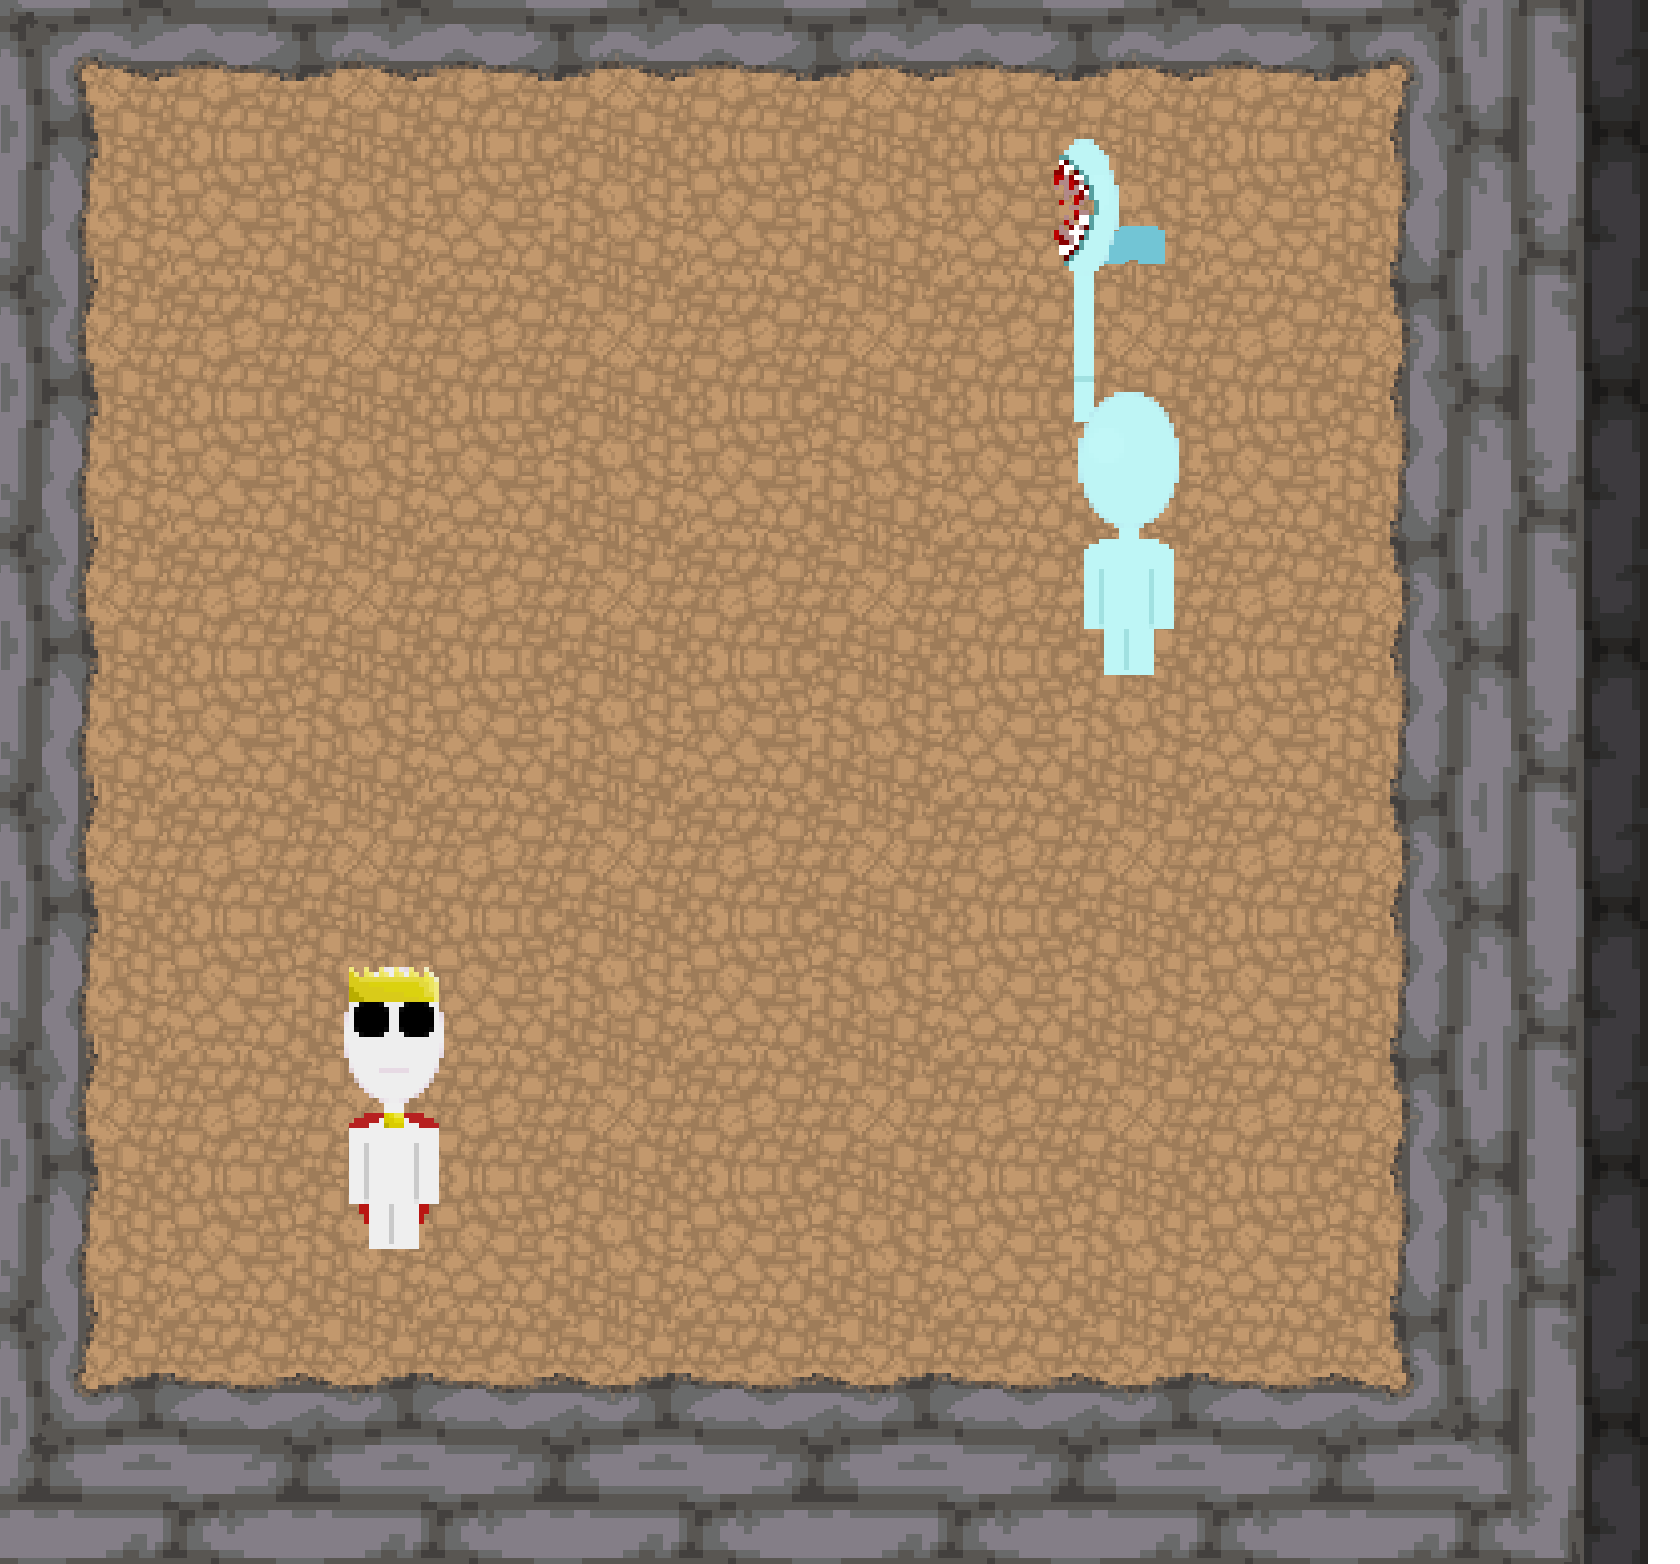
\includegraphics[scale=0.4]{img/Testing/Objective/FollowerAttacking.png}}
                \caption{When faced with an enemy, the follower will automatically attack the enemy}
                \label{fig:FollowerAttacking}
            \end{figure}
            \begin{figure}[hbt!]
                \centerline{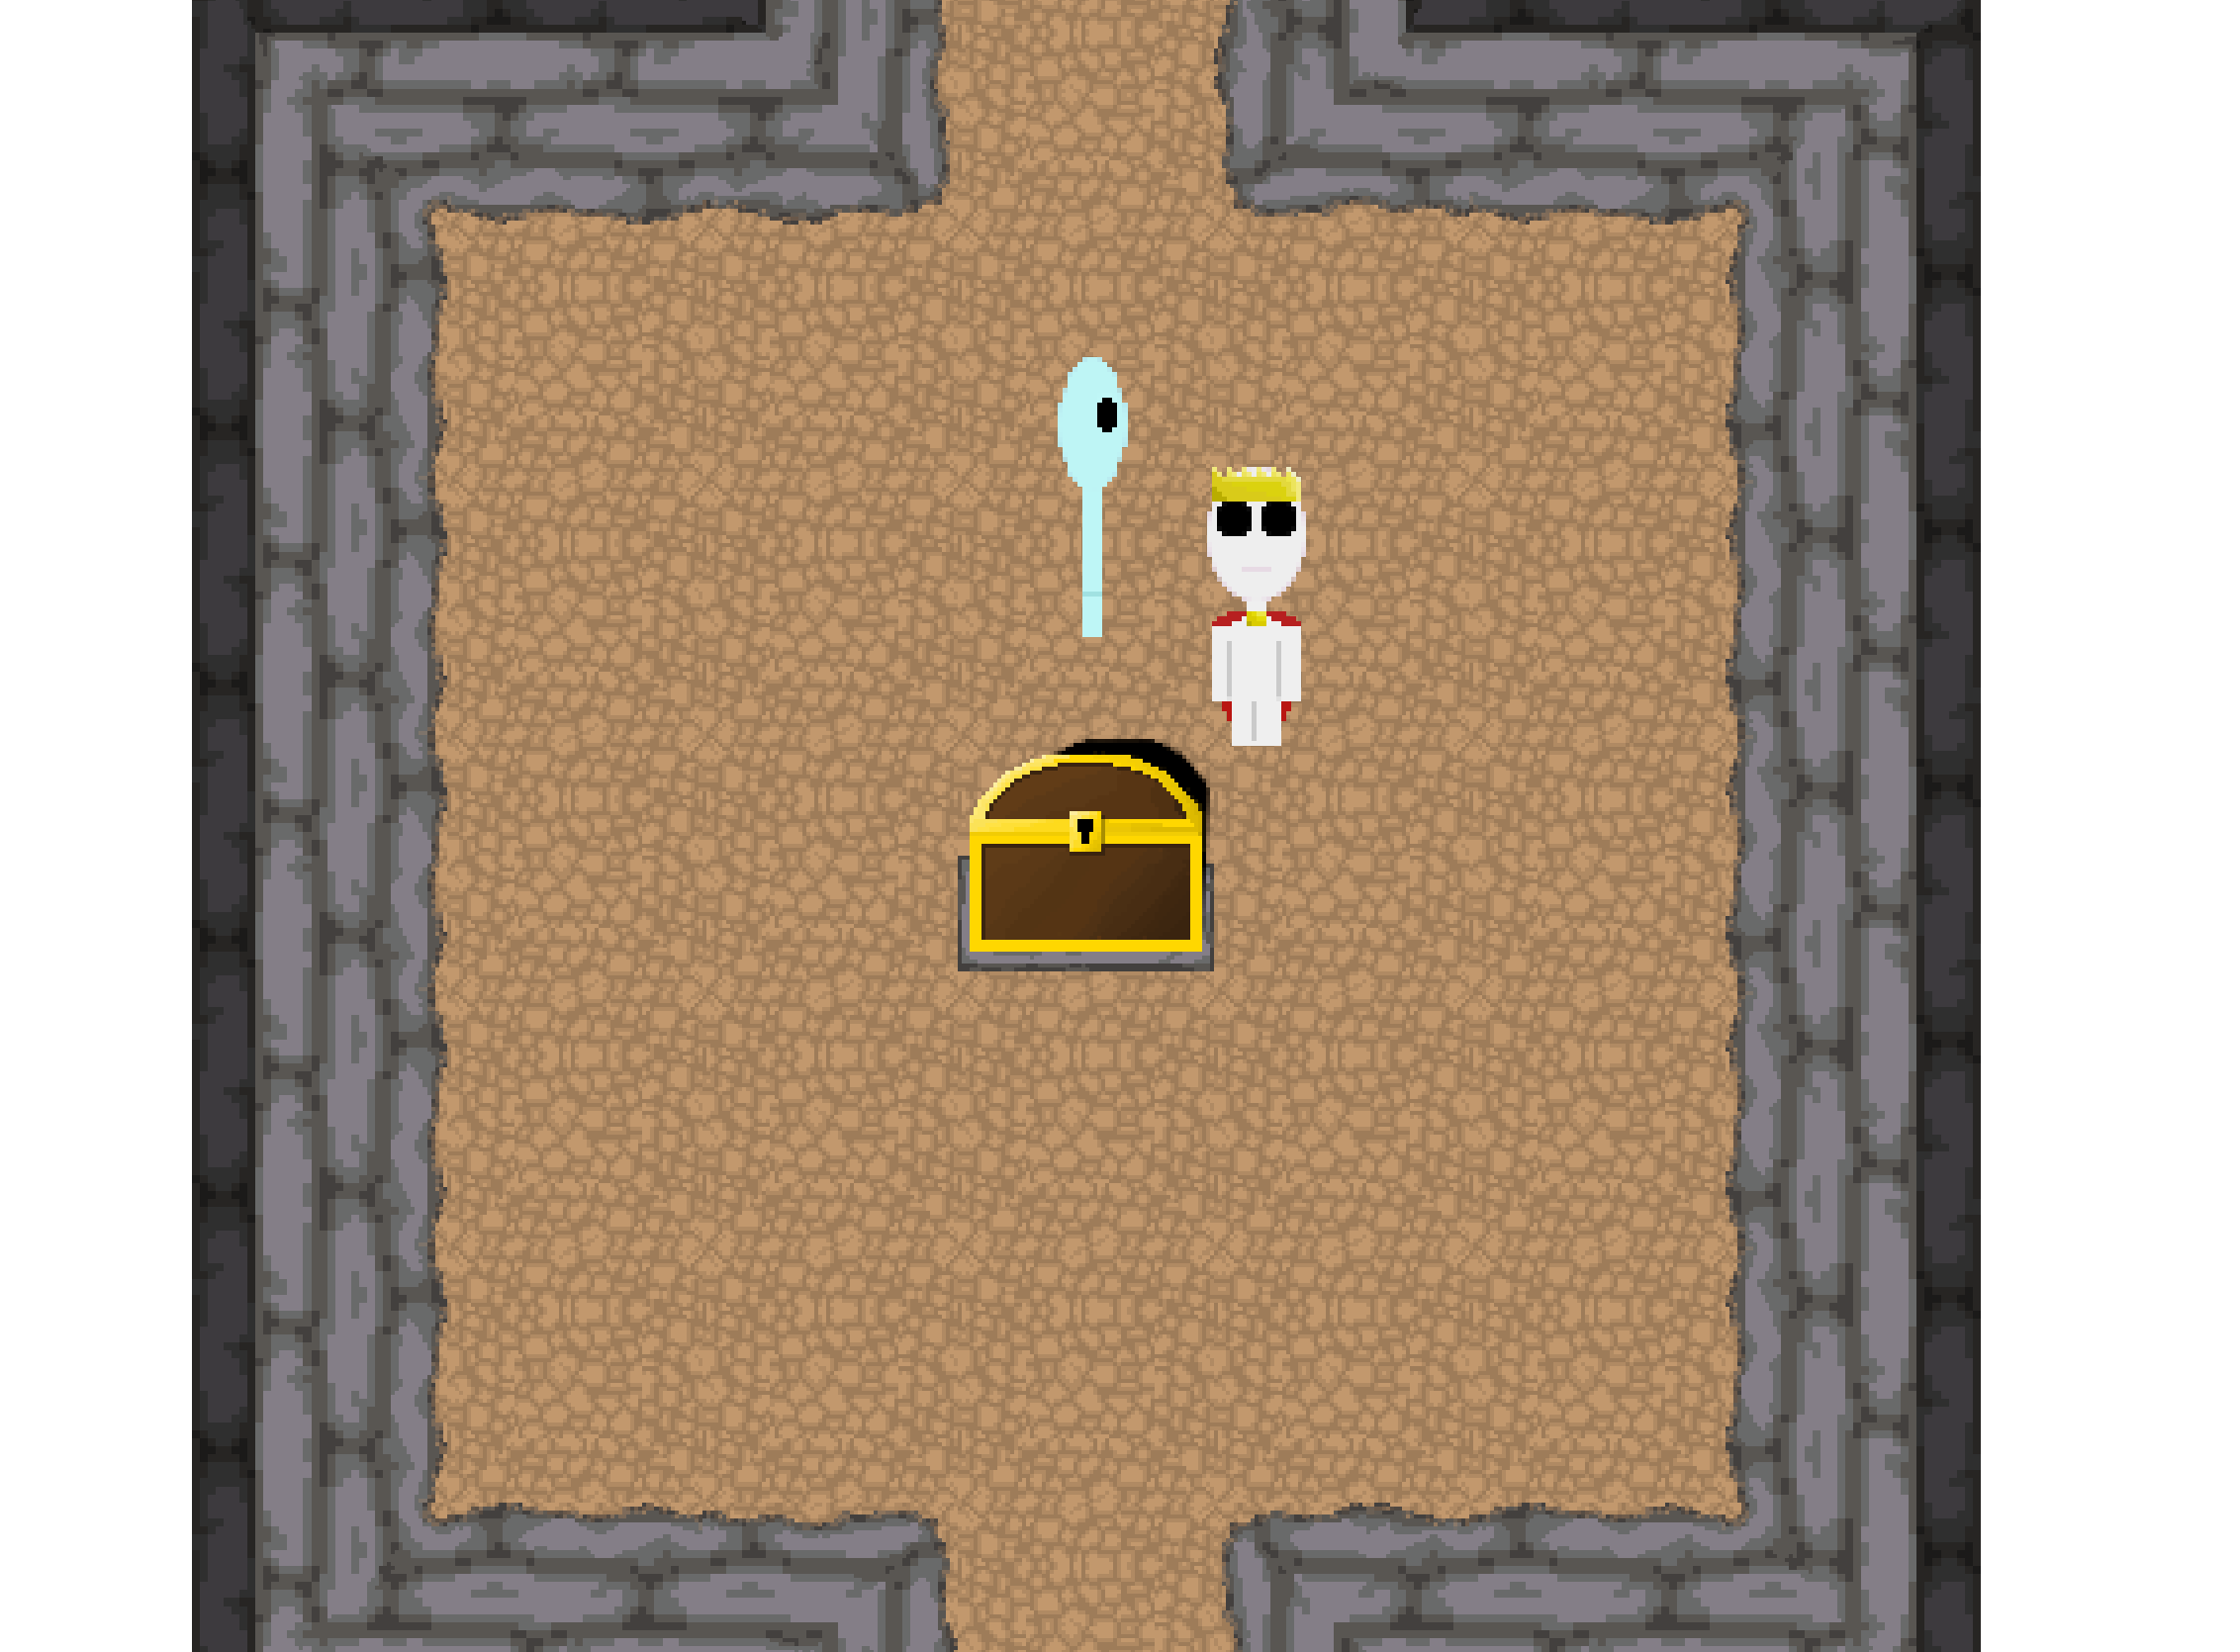
\includegraphics[scale=0.3]{img/Testing/Objective/ChestRoom.png}}
                \caption{Chest Room}
                \label{fig:ChestRoom}
            \end{figure}
            \begin{figure}[hbt!]
                \centerline{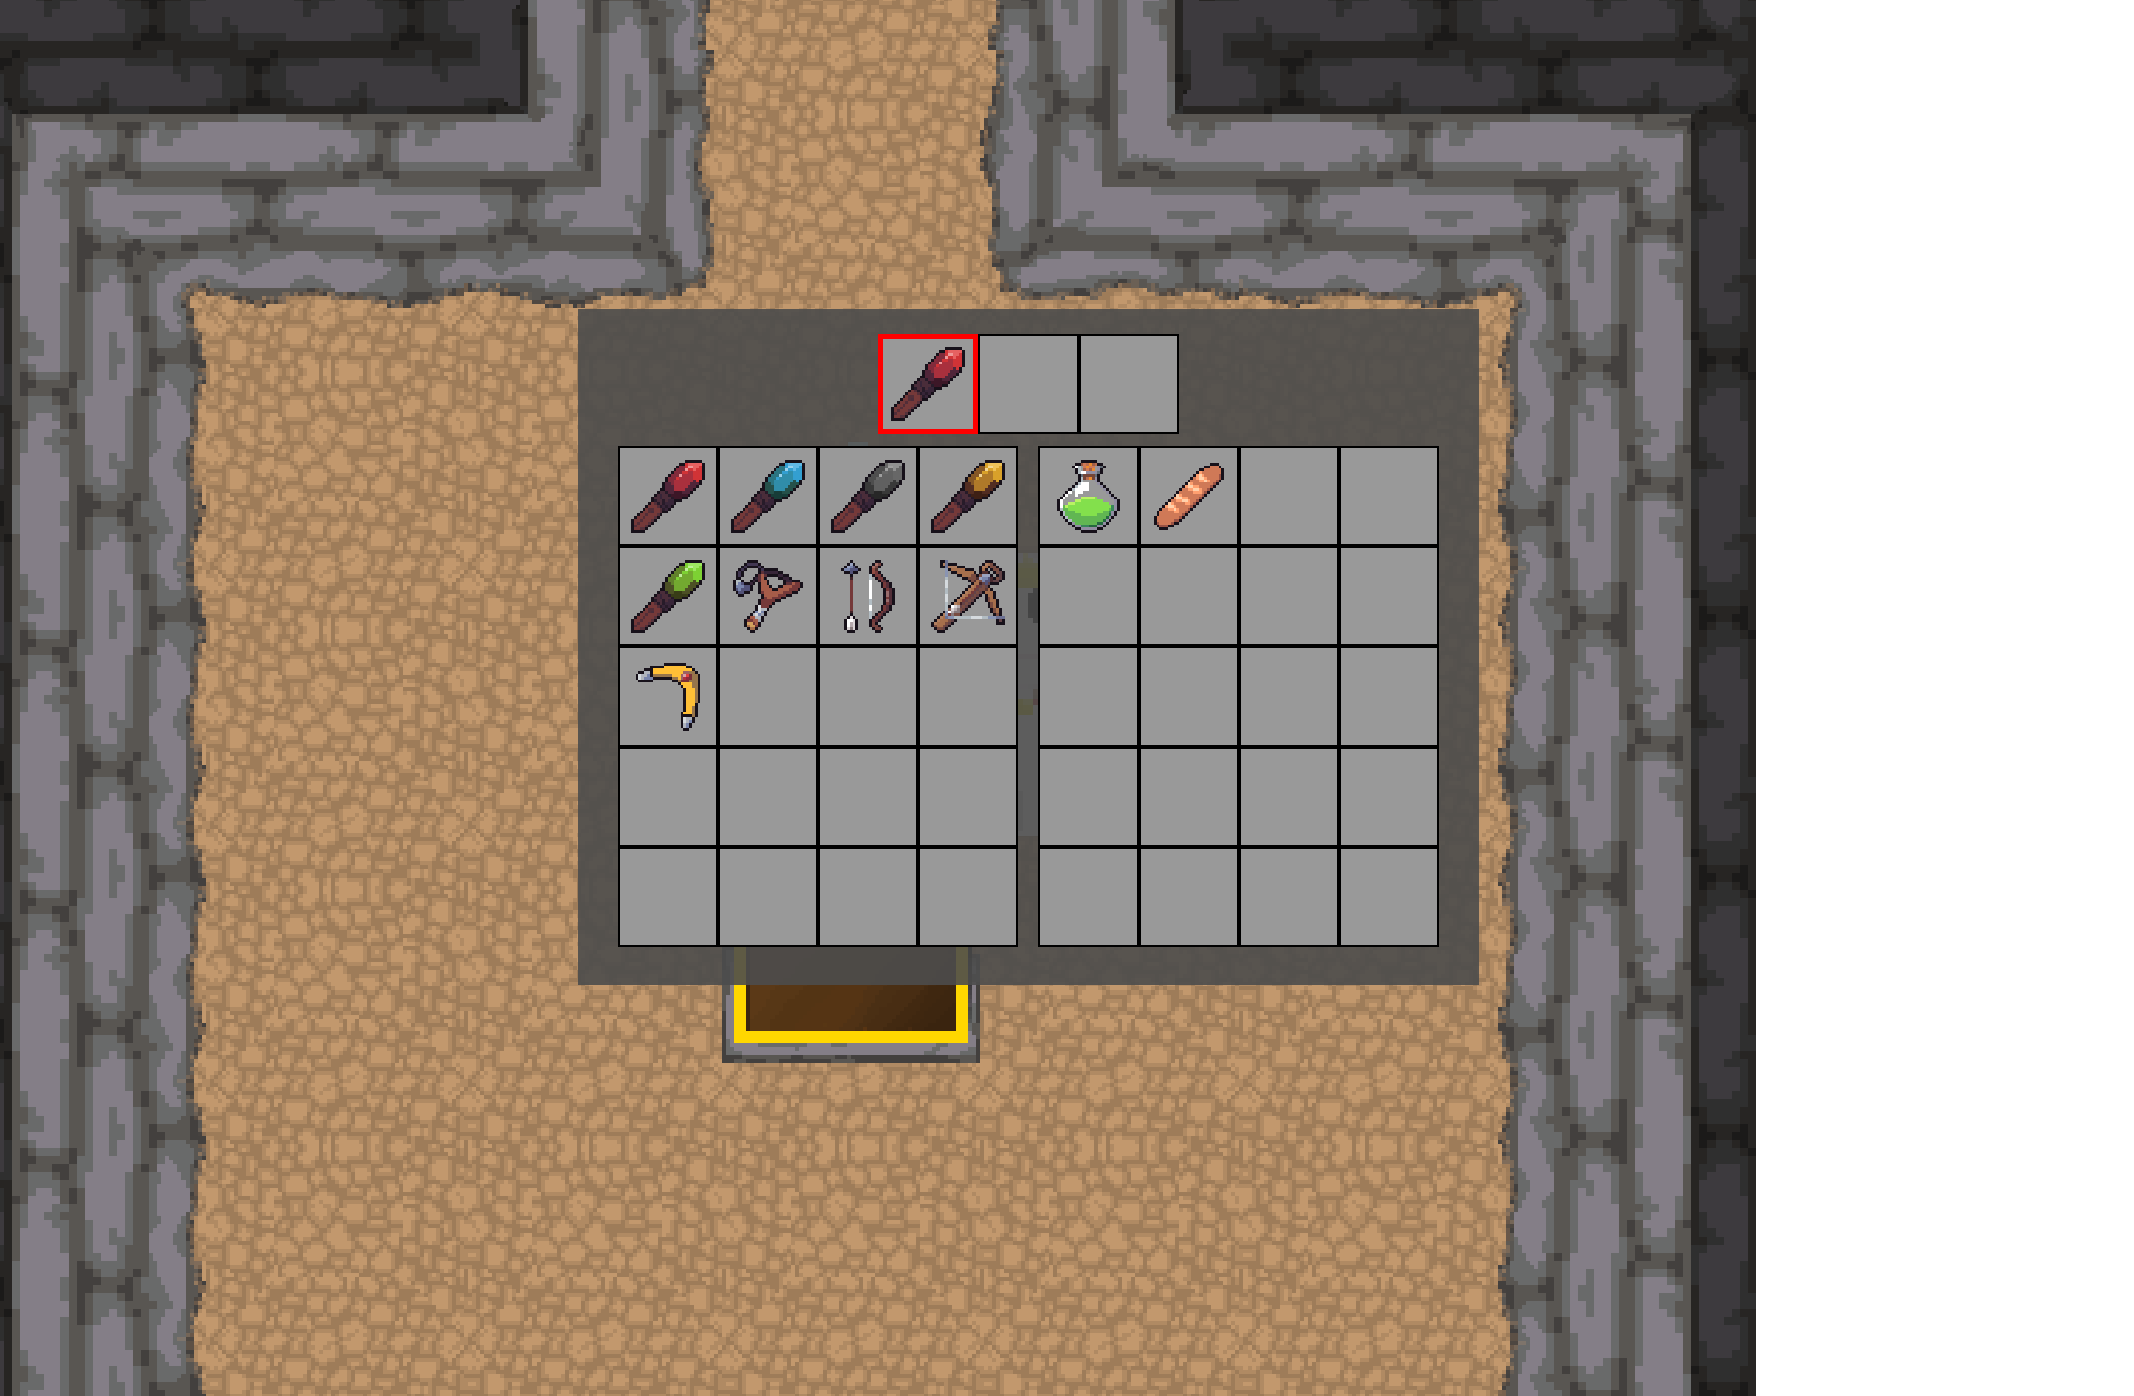
\includegraphics[scale=0.3]{img/Testing/Objective/ChestRoomInventory.png}}
                \caption{Chest Room Inventory}
                \label{fig:ChestRoomInventory}
            \end{figure}
            \begin{figure}[hbt!]
                \centerline{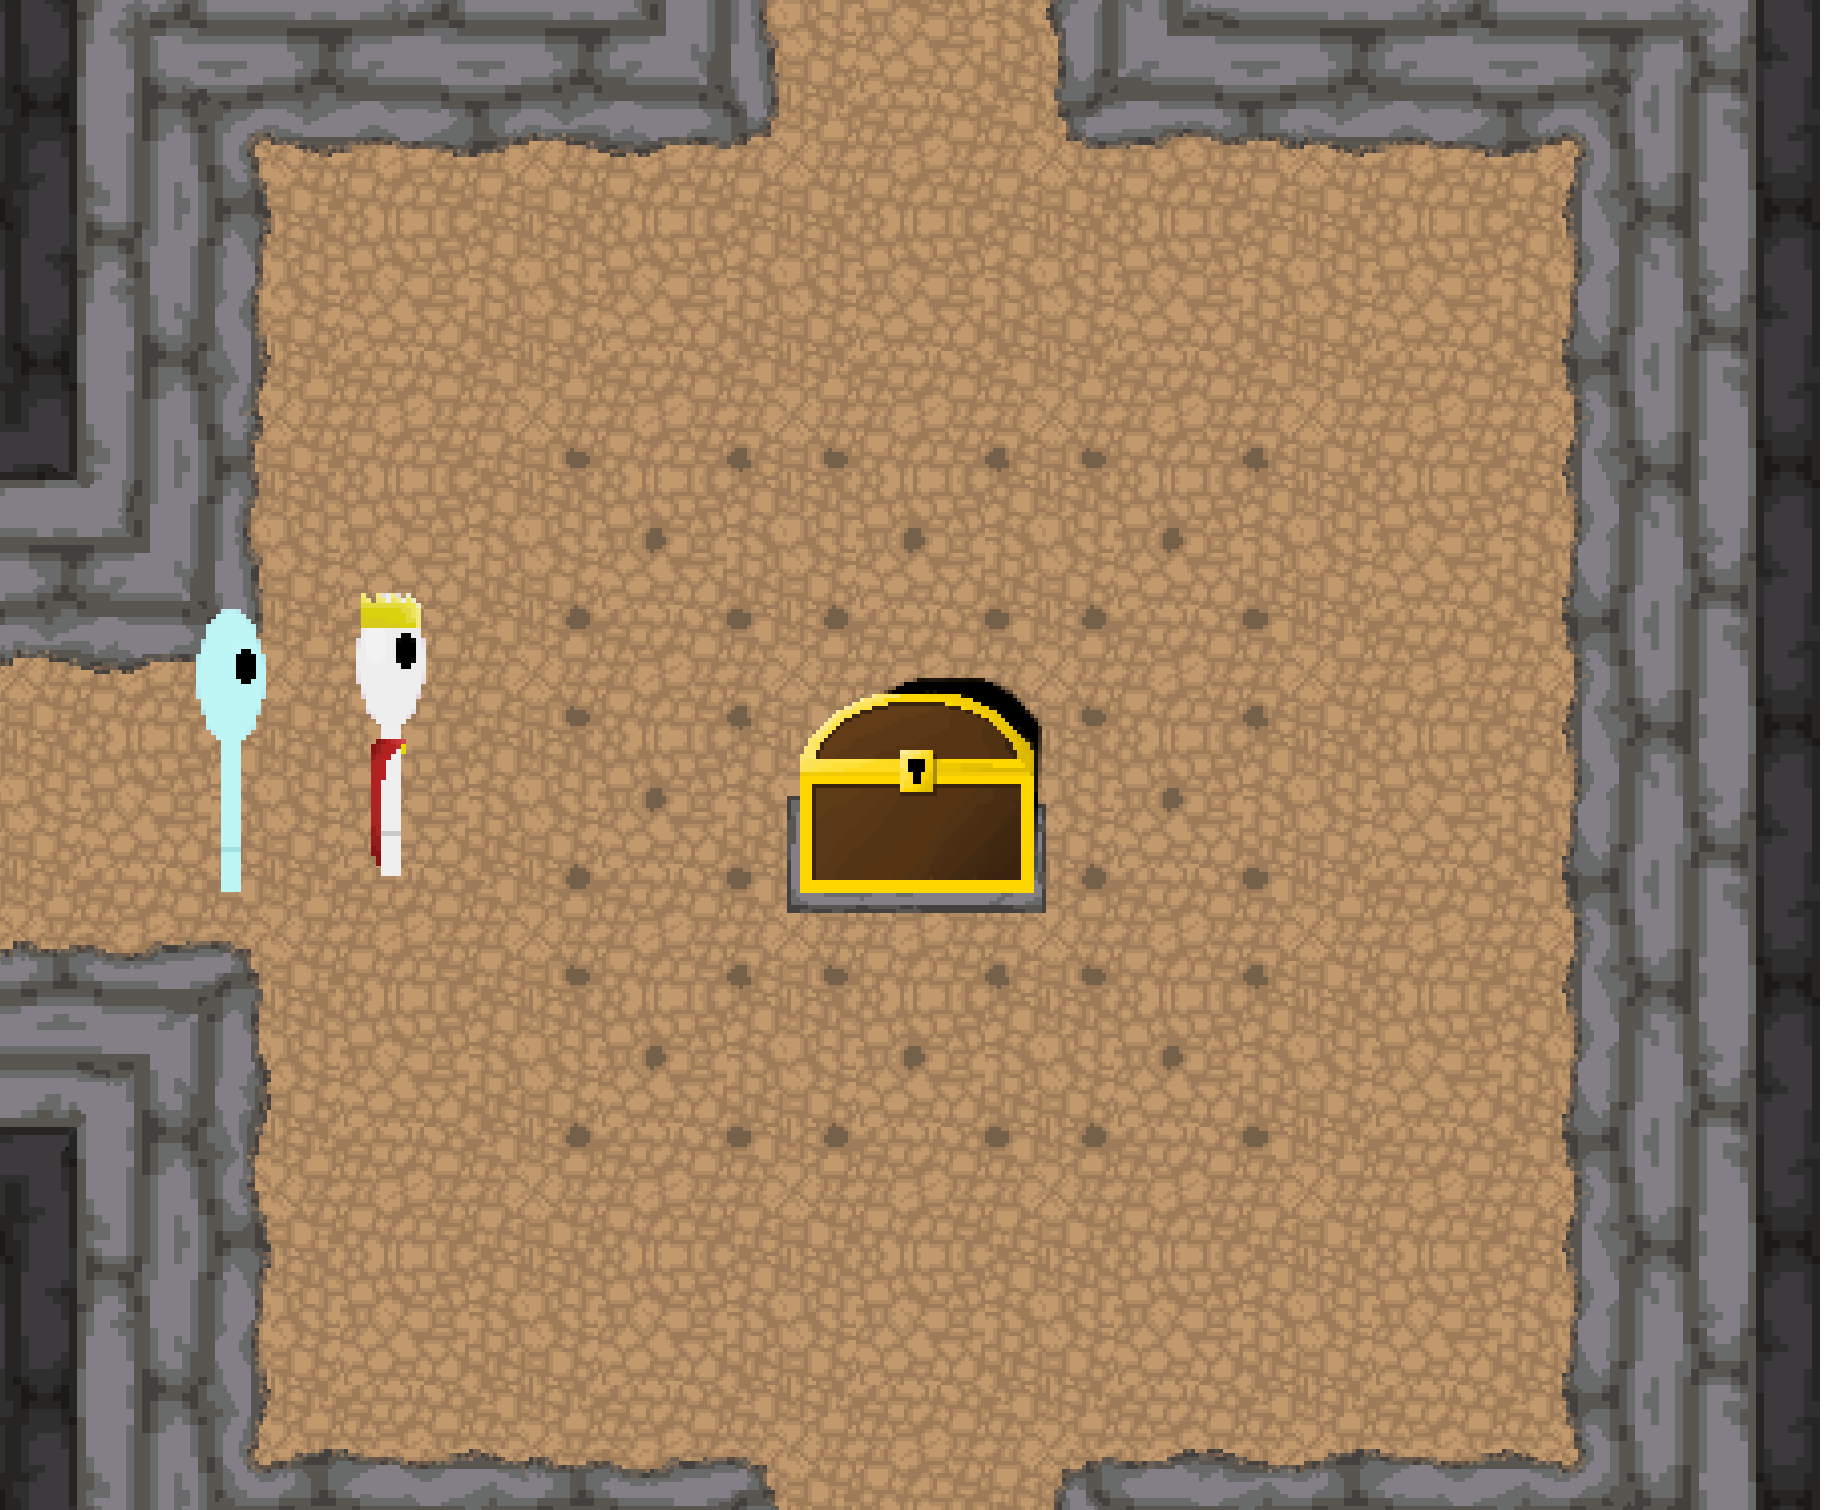
\includegraphics[scale=0.4]{img/Testing/Objective/TrapRoom.png}}
                \caption{Trap room, you cannot click on the chest, however if you stand on the trap it will attack}
                \label{fig:TrapRoom}
            \end{figure}
            \begin{figure}[hbt!]
                \centerline{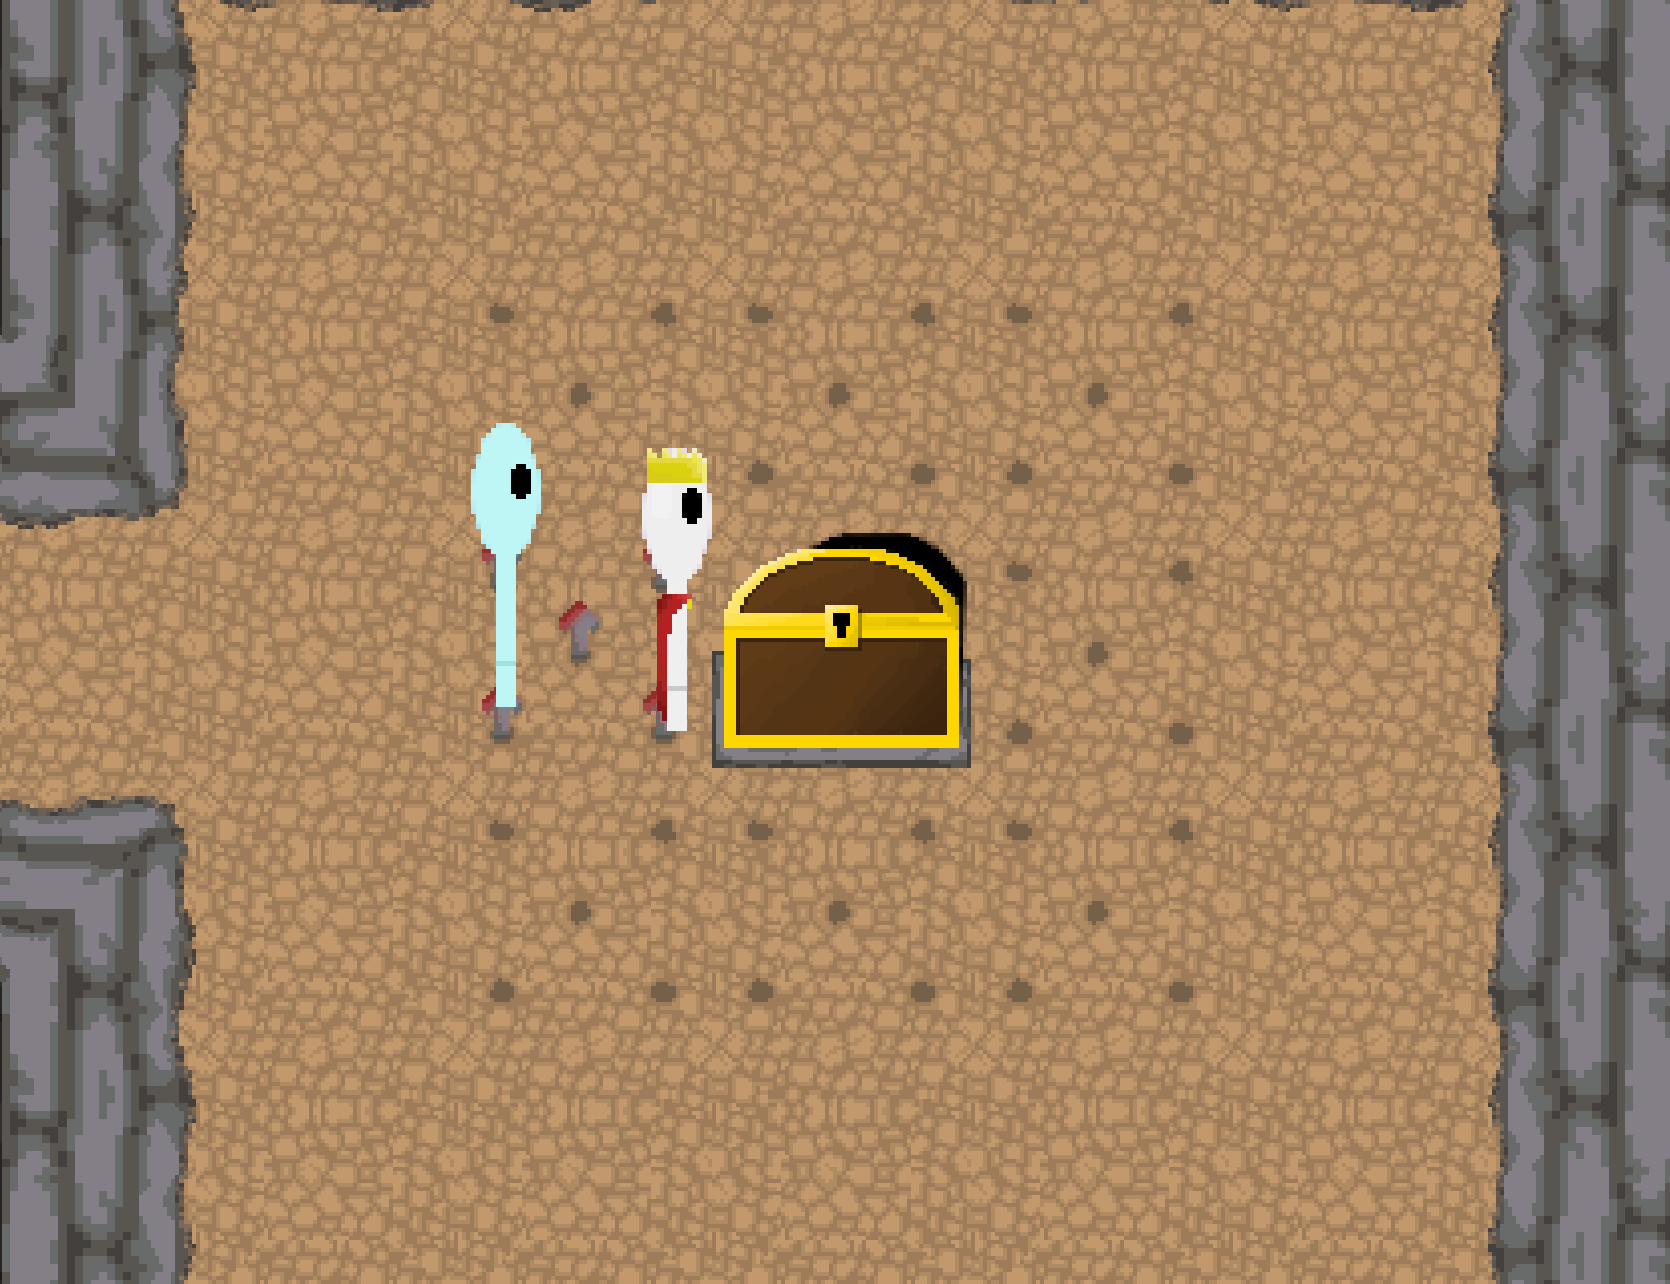
\includegraphics[scale=0.4]{img/Testing/Objective/TrapRoomAttack.png}}
                \caption{When you stand on the spikes, they will start attacking, dealing damage to the player}
                \label{fig:TrapRoomAttack}
            \end{figure}
            \begin{figure}[hbt!]
                \centerline{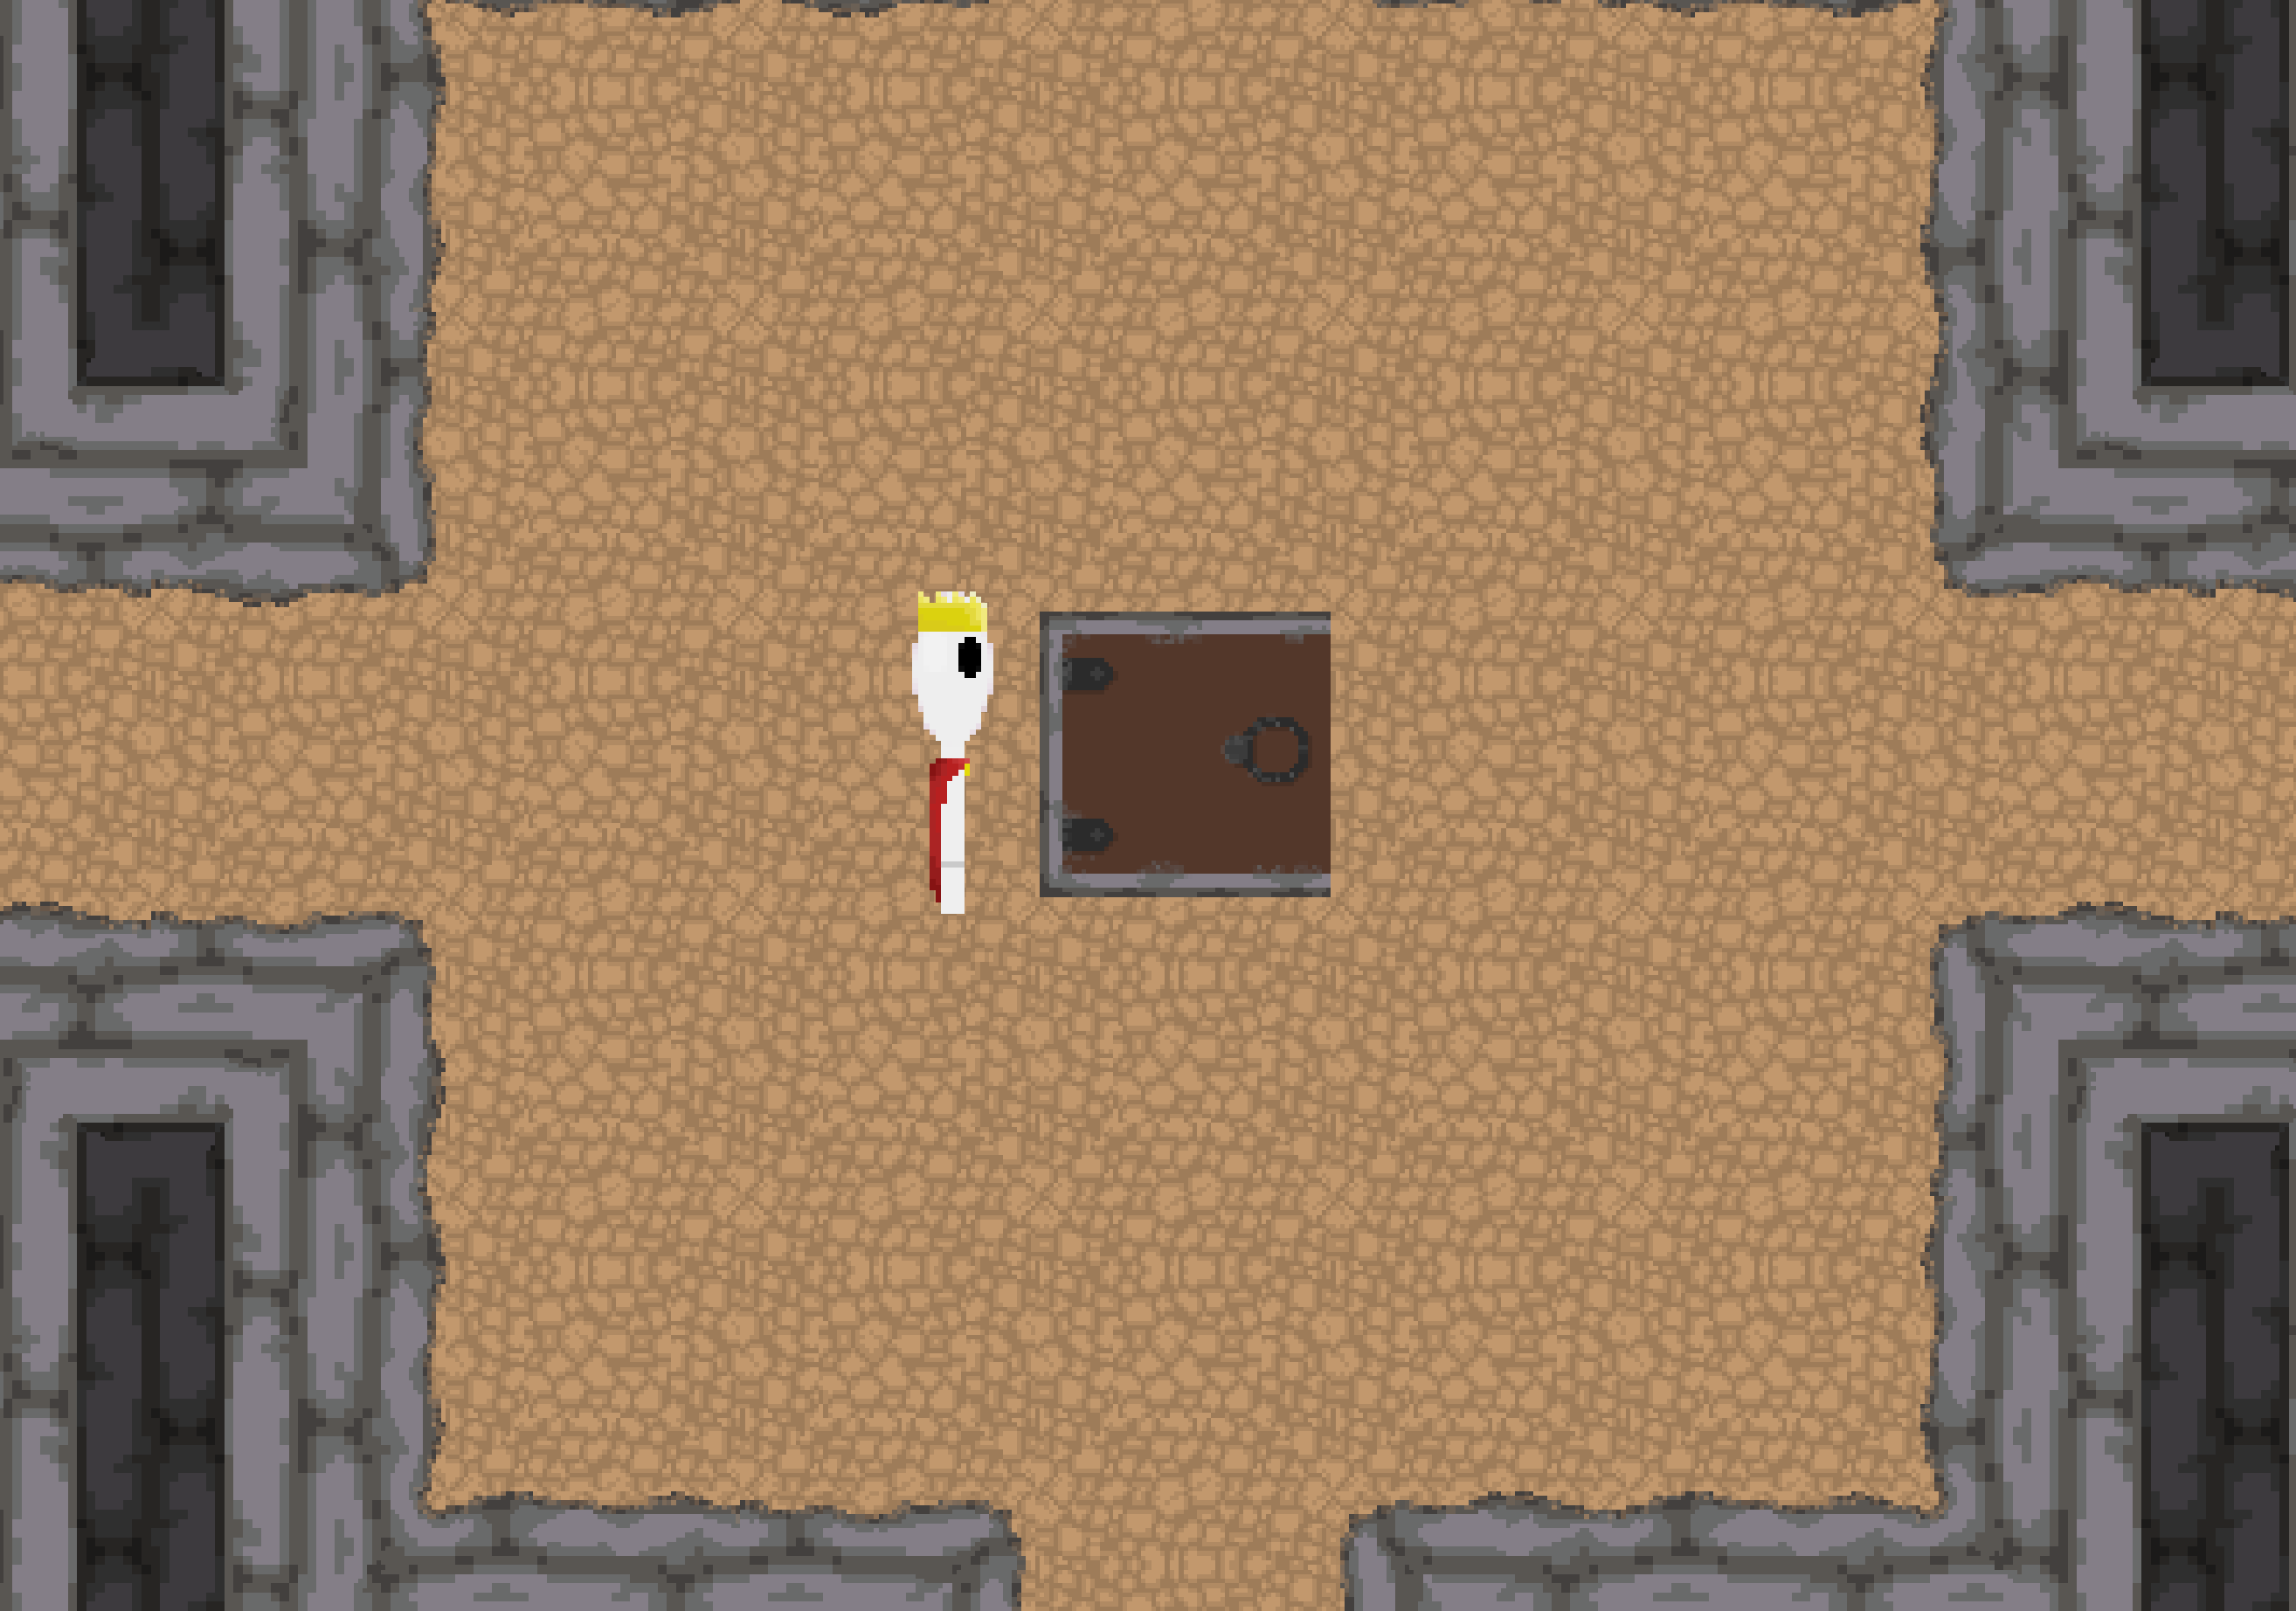
\includegraphics[scale=0.4]{img/Testing/Objective/TrapDoorRoom.png}}
                \caption{Trapdoor room, which you then click on to win the game}
                \label{fig:TrapdoorRoom}
            \end{figure}
            \begin{figure}[hbt!]
                \centerline{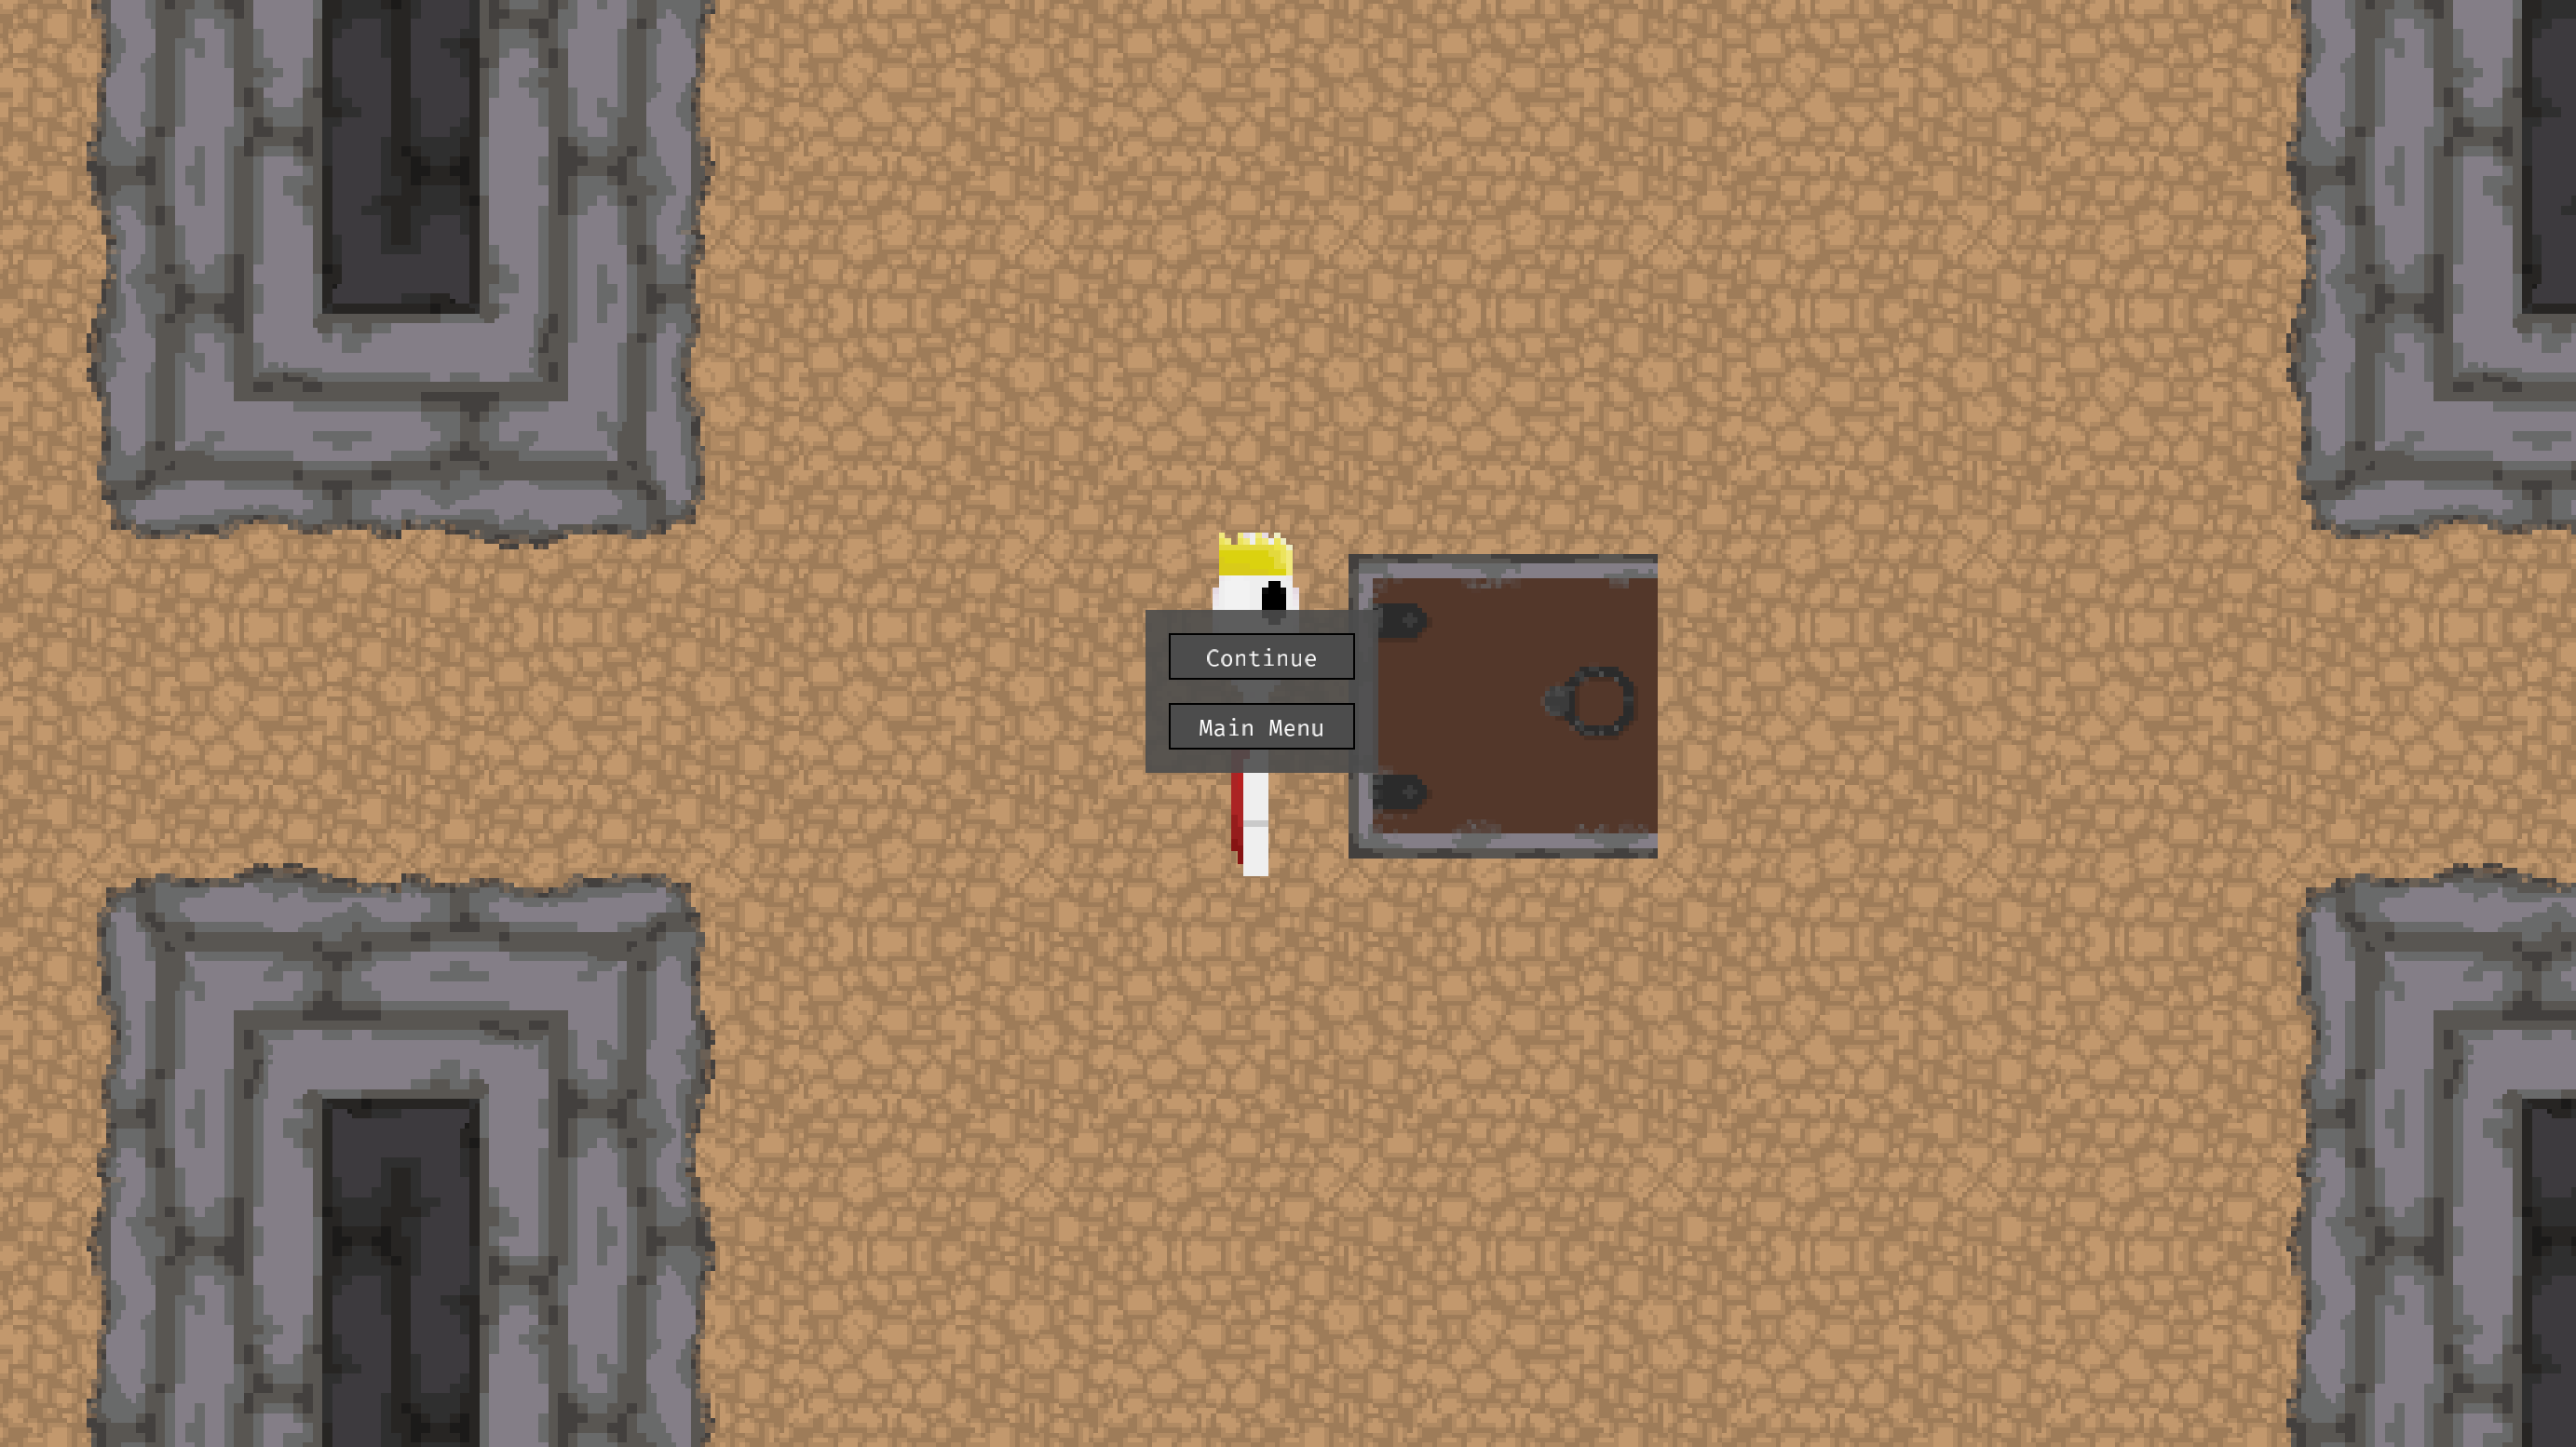
\includegraphics[scale=0.4]{img/Testing/Objective/ExitMenu.png}}
                \caption{Exit menu for pausing the game}
                \label{fig:ExitMenu}
            \end{figure}
            \begin{figure}[hbt!]
                \centerline{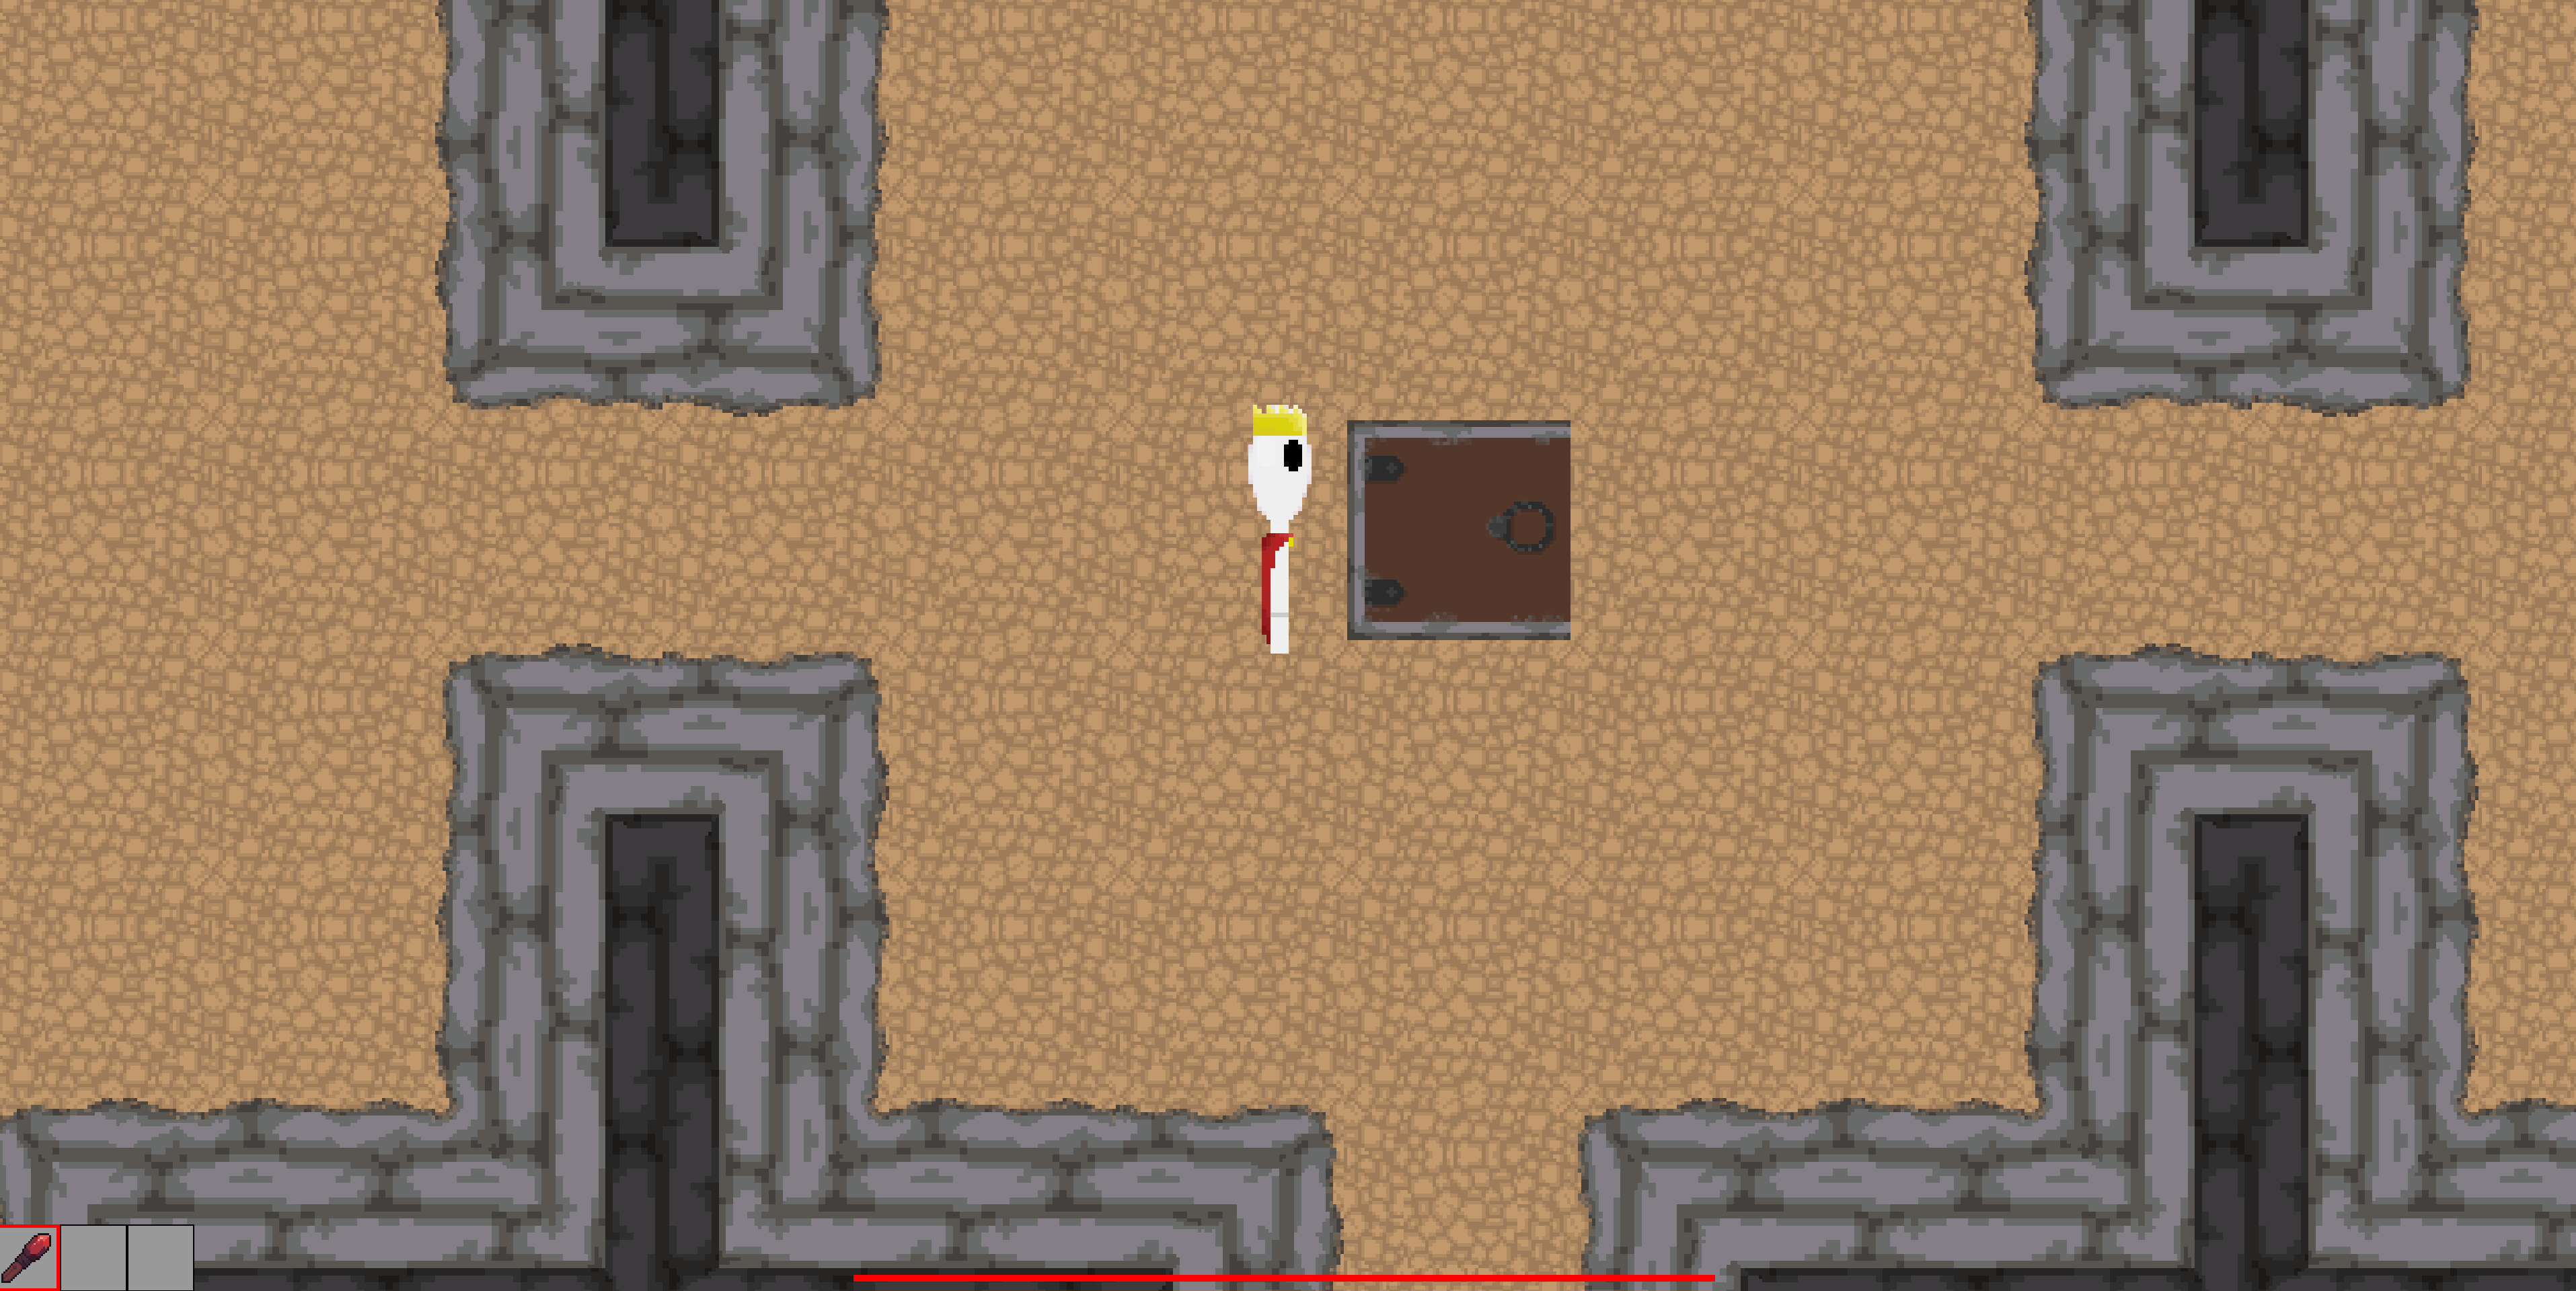
\includegraphics[scale=0.4]{img/Testing/Objective/GUI.png}}
                \caption{GUI overlay for when playing the game, showing the player's health and weapons}
                \label{fig:GUI}
            \end{figure}
            \begin{figure}[hbt!]
                \centerline{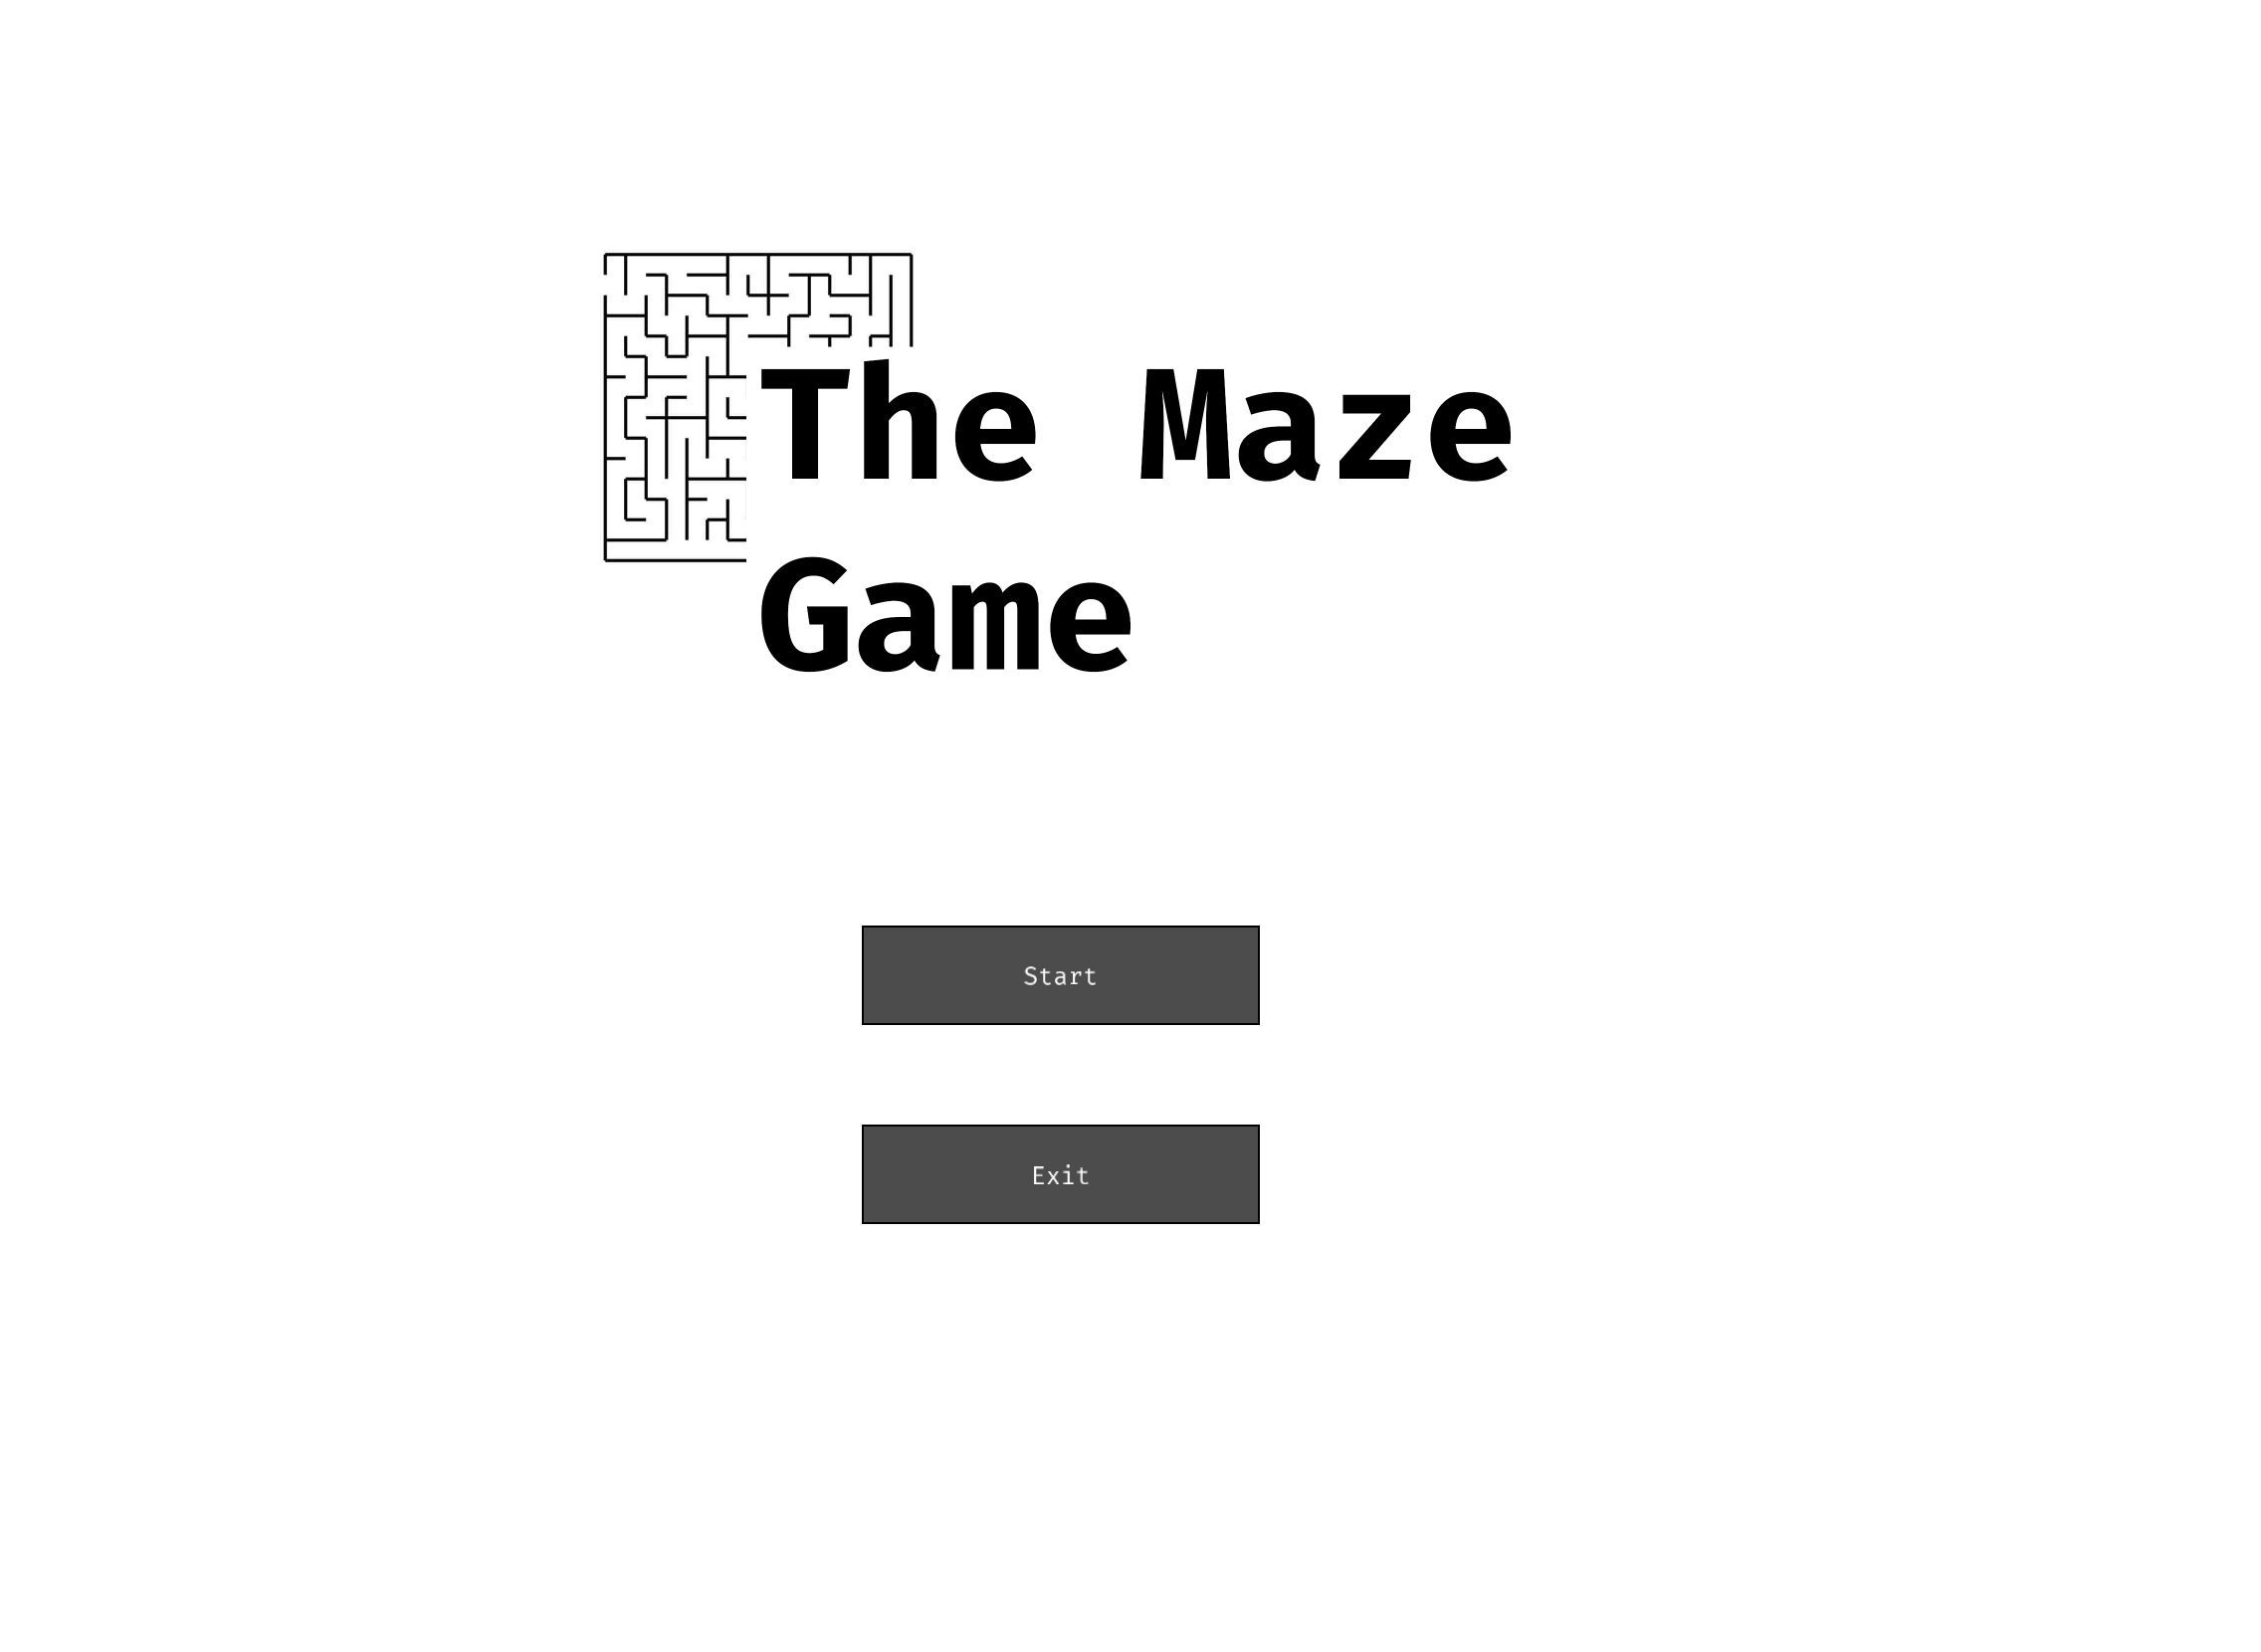
\includegraphics[scale=0.6]{img/Testing/Objective/MainMenu.png}}
                \caption{Main Menu of the game}
                \label{fig:MainMenu}
            \end{figure}
            \begin{figure}[hbt!]
                \centerline{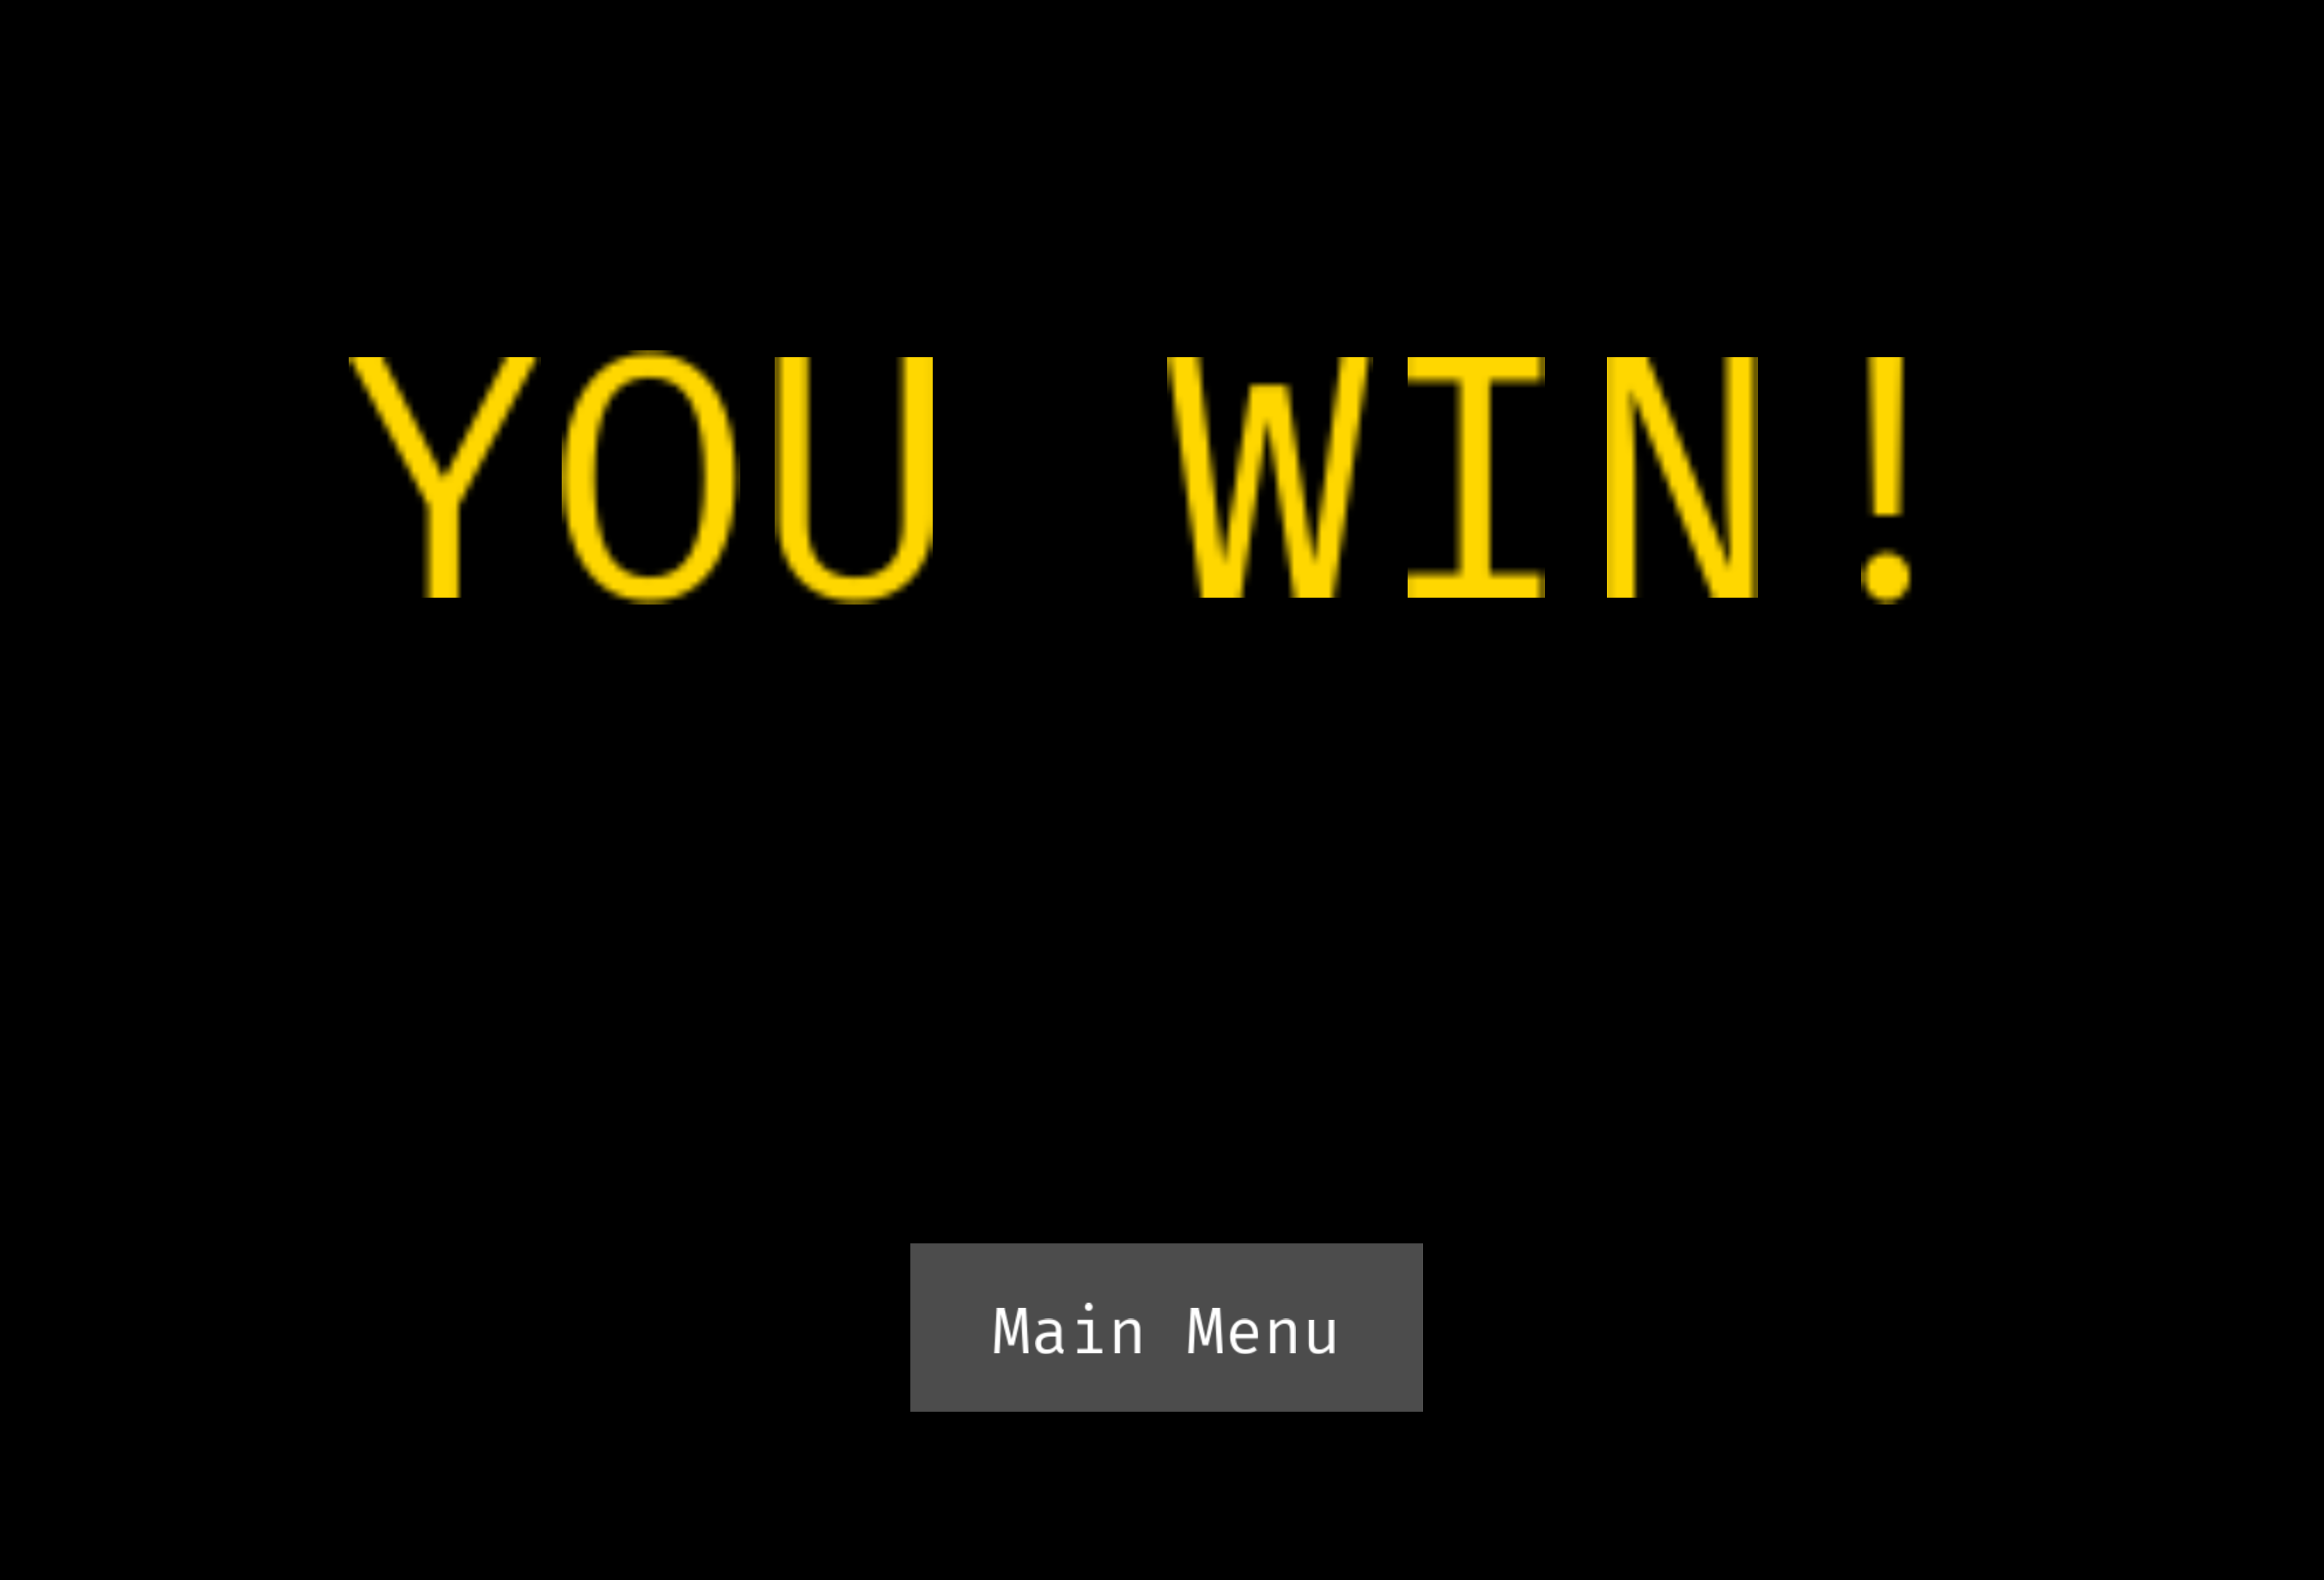
\includegraphics[scale=0.4]{img/Testing/Objective/WinMenu.png}}
                \caption{The menu that is shown when the player wins the game}
                \label{fig:WinMenu}
            \end{figure}
            \clearpage
            \begin{figure}[hbt!]
                \centerline{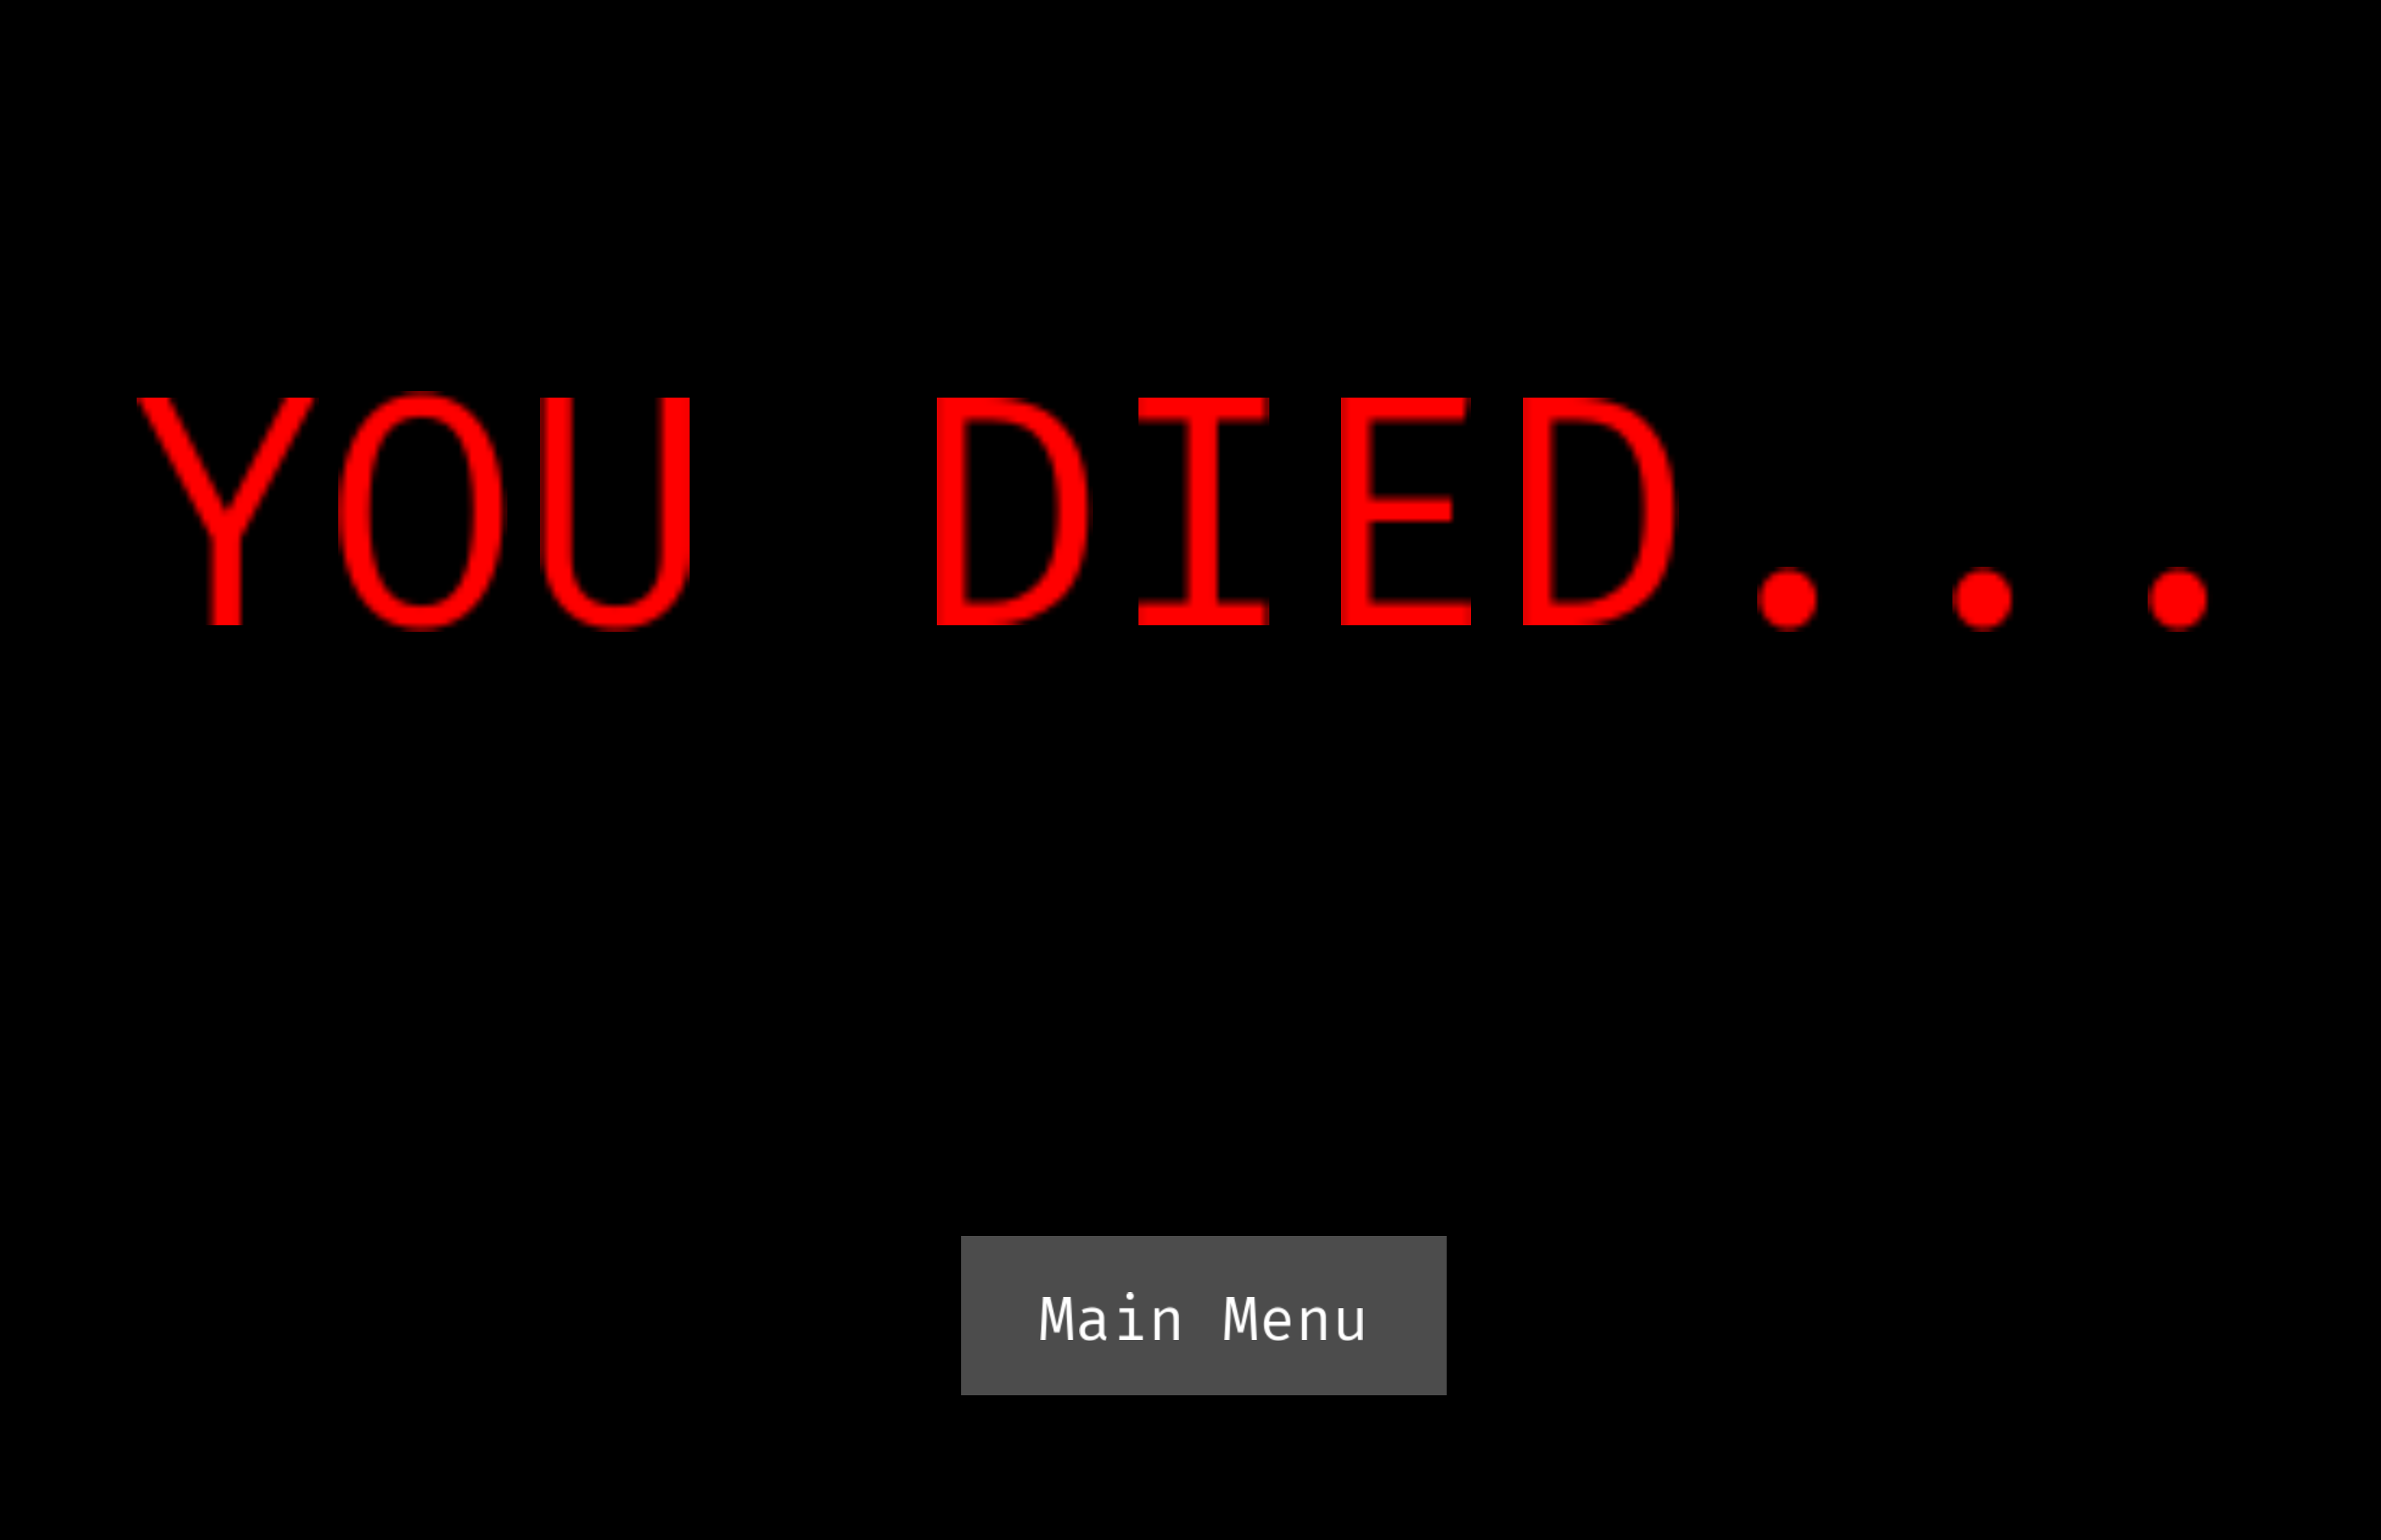
\includegraphics[scale=0.4]{img/Testing/Objective/DeathMenu.png}}
                \caption{The menu that is shown when the player dies}
                \label{fig:DeathMenu}
            \end{figure}
        \subsubsection{Table}
            \begin{center}
                \begin{tabular}{ | m{0.2\textwidth} | m{0.5\textwidth} | m{0.1\textwidth} | m{0.1\textwidth} | }
                    \hline
                    \textbf{Objective} & \textbf{Expected Outcome} & \textbf{Passed?} & \textbf{Figures} \\
                    \hline
                    Have an effective rendering system & Have camera that can move around using OpenGL and be able to render a tile or object on the screen. & Yes & All \\
                    \hline
                    Be able to generate an infinite maze & Have a maze that can generate rooms and procedurally generated as the player moves around. & Yes & \ref{fig:FullMaze}\\
                    \hline
                    Create NPCs that rome the maze and can start following you & The player should be able to find NPCs, in the maze roaming around, and once clicked, should be able to get them to follow the player around using the A* algorithm. & Yes & \ref{fig:Follower}, \ref{fig:FollowerQuestion}, \ref{fig:FollowerFollowing} \\
                    \hline
                    Add items and a way to collect them with a simple space-based inventory system & Have different items in the game which the player can collect with an inventory and pass onto their followers & Yes & \ref{fig:PlayerInventory}, \ref{fig:FollowerInventory} \\
                    \hline
                    Add combat into the game & Allow the player to be able to find enemies in the maze, which will start attacking the player when in close proximity. The player is able to fight back (with their followers automatically attacking the enemy) firing projectiles from different weapons that do damage the the enemy and causes particles to spawn when it hits an object & Yes & \ref{fig:Firing}, \ref{fig:Enemy}, \ref{fig:FollowerAttacking} \\
                    \hline
                    Create different rooms that can be found in the maze. &  Have different rooms, e.g. a chest and trap room, that can be found throughout the maze, also allow the room with the enemy in to automatically close the entrances so that the player cannot escape & Yes & \ref{fig:ChestRoom}, \ref{fig:ChestRoomInventory}, \ref{fig:TrapRoom}, \ref{fig:TrapRoomAttack}, \ref{fig:TrapdoorRoom} \\
                    \hline
                    Create a menu system & Menus should be able to allow the user to navigate through the game, including one for the inventory and main menu. They should also allow the transfer of items between different containers such as a chest or a follower & Yes & \ref{fig:ExitMenu}, \ref{fig:GUI}, \ref{fig:MainMenu}, \ref{fig:WinMenu}, \ref{fig:DeathMenu}, \ref{fig:ChestRoomInventory}, \ref{fig:PlayerInventory}, \ref{fig:FollowerInventory} \\
                    \hline
                    Finalise everything & The sprites should be updated to a medieval theme with more stats for the player to try and attack & Yes & All \\
                    \hline
                \end{tabular}
            \end{center}
\end{document}